\documentclass[12pt]{report}

% Language setting
% Replace `english' with e.g. `spanish' to change the document language
\usepackage[USenglish]{babel}

% Set page size and margins
% Replace `letterpaper' with `a4paper' for UK/EU standard size
\usepackage[letterpaper,top=2cm,bottom=2cm,left=3cm,right=3cm,marginparwidth=1.75cm]{geometry}

% Useful packages
\usepackage{amsmath}
\usepackage{amssymb}
\usepackage{graphicx}
\usepackage{authblk}
\usepackage{times}
\usepackage{epsfig}
\usepackage{dcolumn}
\usepackage{bm}
\usepackage{color}
\usepackage{xcolor}
\usepackage{longtable}
\usepackage{array}
\usepackage{multirow}
\usepackage{enumerate}
\usepackage{booktabs}
\usepackage{stfloats}
\usepackage{fancyhdr}
\usepackage{slashed}
\usepackage{feynmp-auto}
\usepackage[normalem]{ulem}
\usepackage{titlesec}
\usepackage{tocloft}
\usepackage{hyperref}
\hypersetup{
    colorlinks=true,
    linkcolor=blue,      % 设置内部链接(如目录项)的颜色
    citecolor=green,     % 设置引用的颜色
    filecolor=magenta,   % 设置文件链接的颜色
    urlcolor=black         % 设置网址链接的颜色
}
%%%%%%%%%%%%%%%%%%%%%%%%%%%%%%%%%%%%%%%%%%%%%%%%%%%%%%%%%%%%%%%
\newcommand{\tev}{\rm TeV}
\newcommand{\gev}{\rm GeV}
\newcommand{\gevc}{{\rm GeV}/c}
\newcommand{\gevcs}{{\rm GeV}/c^2}
\newcommand{\mev}{\rm MeV}
\newcommand{\mevcs}{{\rm MeV}/c^2}
\newcommand{\kev}{\rm KeV}
\newcommand{\kevcs}{\kev/c^2}
\newcommand{\ev}{\rm eV}
\newcommand{\protonp}{p^+}
\newcommand{\pip}{\pi^+}
\newcommand{\piz}{\pi^0}
\newcommand{\pim}{\pi^-}
\newcommand{\kew}{\rm K}
\newcommand{\dd}{{\rm d}}
%%%%%%%%%%%%%%%%%%%%%%%%%%%%%%%%%%%%%%%%%%%%%%%%%%%%%%%%%%%%%%%
\newcounter{problemname}
\numberwithin{problemname}{chapter}
\newenvironment{problem}{\vspace{1em}\stepcounter{problemname}\par\noindent {\large\textbf{\textsc{Problem \thechapter.\arabic{problemname}}}} \par\color{blue}}{\par}
\newenvironment{solution}{\vspace{1em}\par\noindent{\large\textbf{\textsc{Solution}}}\par}{\vspace{1em}\hrule}
%%%%%%%%%%%%%%%%%%%%%%%%%%%%%%%%%%%%%%%%%%%%%%%%%%%%%%%%%%%%%%%
\renewcommand{\thefootnote}{\fnsymbol{footnote}}

% \title{Solutions to Homework Problems from the \\{\it Particle Physics} Course Delivered by Ying Chen}
% \author[1,2]{Yan-Feng Li\thanks{E-mail: liyanfeng24@mails.ucas.ac.cn}}

% \affil[1]{Institute of High Energy Physics, Beijing 100049, China}
% \affil[2]{University of Chinese Academy of Sciences, Beijing 100049, China}

% \renewcommand*{\Affilfont}{\it}


% 设置章节标题居中
\titleformat{\chapter}[display]
  {\normalfont\huge\bfseries\centering} % 标题字体和大小,且居中
  {\chaptername\ \thechapter} % 章节编号
  {20pt} % 标题与章节内容的间距
  {\centering} % 标题居中
\renewcommand{\cftsecfont}{\large} % 段落标题的字体大小
\renewcommand{\cftsecpagefont}{\large} % 段落页码的字体大小
\renewcommand{\cftchapfont}{\Large} % 章节标题的字体大小
\renewcommand{\cftchappagefont}{\Large} % 章节页码的字体大小
\allowdisplaybreaks
\begin{document}
\begin{titlepage}
    \centering
    \href{https://www.ucas.ac.cn/}{
    \includegraphics[width=0.4\textwidth]{UCAS_LOGO.png}
    }\quad\quad
    \href{https://www.ihep.cas.cn/}{
    \includegraphics[width=0.53\textwidth]{IHEP_LOGO.png}
    }\\[0.8cm]
    % 学校名称
    {\Large \href{https://www.ucas.ac.cn/}{\textbf{\textsc{University of Chinese Academy of Sciences}}}} \\[0.2cm]
    {\Large \href{https://mooc.mooc.ucas.edu.cn/mooc-ans/course/350140000013009.html?clazzId=350140000017216}{\textbf{\textsc{quantum field theory, autumn 2024}}}} \\[5cm]

    % 标题
    {\LARGE \it \textbf{Solutions to Homework Problems from the \\[0.5cm] \href{https://mooc.mooc.ucas.edu.cn/mooc-ans/course/350140000013009.html?clazzId=350140000017216}{Quantum Field Theory Course} Delivered by \href{https://people.ucas.edu.cn/~jiay}{Yu JIA}}} \\[1.5cm]

    % 作者信息
    {\Large Yan-Feng Li\footnote{E-mail: liyanfeng24@mails.ucas.ac.cn}} \\[0.5cm]

    % 机构
    {\large \it \href{https://www.ihep.cas.cn/}{Institute of High Energy Physics}, Beijing 100049, China} \\[0.2cm]
    {\large \it \href{https://www.ucas.ac.cn/}{University of Chinese Academy of Sciences}, Beijing 100049, China} \\[1cm]

    % 日期
    {\large \today}
\end{titlepage}
% \maketitle
\pagestyle{fancy}
\setlength{\headheight}{14.5pt}
\fancypagestyle{plain}{
    \fancyhf{}
    \fancyfoot[C]{-\enspace\thepage\enspace-}
    \renewcommand{\headrulewidth}{0pt}
}
\renewcommand{\headrulewidth}{0.4pt}
\pagenumbering{gobble}
\newpage
\pagenumbering{roman}
\tableofcontents
\newpage
\pagenumbering{arabic}
\setcounter{page}{1}
\fancyfoot{}
\fancyfoot[C]{-\enspace\thepage\enspace-}
%%%%%%%%%%%%%%%%%%%%%%%%%%%%%%%%%%%%%%%%%%%%%%%%%%%%%%%%%%%%%%%%%%%%%%
\chapter{Classical Field}
\begin{problem}
Solve energy levels of hydrogen atom by utilizing Klein-Gordon Equation.
\\
\end{problem}

\begin{solution}
The potential four-vector in hydrogen atom is
\begin{equation}
    A^\mu=(\phi,\mathbf{A}),
\end{equation}
where $\phi=e/r$ and $\mathbf{A}=0$.
\par
According to the principle of minimal coupling, the four-momentum $p^\mu$ is replaced with $p^\mu-qA^\mu$, where $q$ is the charge of the particle ($q=-e$ for electron). Thus we have
\begin{equation}
    (E-q\phi)^2=\mathbf{p}^2+m^2.
\end{equation}
\par
With $\mathbf{p}\rightarrow -i\nabla$, the time-independent Klein-Gordon Equation in Coulomb potential is obtained, that is
\begin{equation}
    \{\nabla^2+(E-q\phi)^2-m^2\}\psi=0.
\end{equation}
\par
It's convenient to simplify the equation above in the spherical coordinate:
\begin{equation}
    \{\frac{1}{r^2}\frac{\partial}{\partial r}(r^2\frac{\partial}{\partial r})+\frac{1}{r^2\sin{\theta}}\frac{\partial}{\partial\theta}(\sin{\theta}\frac{\partial}{\partial\theta})+\frac{1}{r^2\sin^2{\theta}}\frac{\partial^2}{\partial \varphi^2}+(E+\frac{e^2}{r})^2-m^2\}\psi=0.
\end{equation}
\par
We can separate the radial variable ($r$) from angular variables ($\theta, \varphi$) so that we get two equations:
\begin{equation}
    \{\frac{\dd}{\dd r}(r^2\frac{\dd}{\dd r})+r^2[(E+\frac{e^2}{r})^2-m^2]\}R(r)=\mathbf{L}^2R(r),\label{radial}
\end{equation}
\begin{equation}
    -\{\frac{1}{\sin{\theta}}\frac{\partial}{\partial\theta}(\sin{\theta}\frac{\partial}{\partial\theta})+\frac{1}{\sin^2{\theta}}\frac{\partial^2}{\partial \varphi^2}\}Y(\theta, \varphi)=\mathbf{L}^2Y(\theta, \varphi).
\end{equation}
The $\mathbf{L}^2$ can be solved to be $l(l+1)$, $l=0, 1, 2, ...$ is the quantum number of orbit angular momentum.Thus Eq. \eqref{radial} becomes
\begin{equation}
    \{\frac{\dd^2}{\dd r^2}+[(E+\frac{e^2}{r})^2-\frac{l(l+1)}{r^2}-m^2]\}u(r)=0,\label{NotSimplifyEq}
\end{equation}
where we have substituted $R(r)$ with $u(r)/r$. Instead of mathematics tricks, there is a physical motivation for replacing $R(r)$ with $u(r)$: we hope the wave-function should be normalized:
\begin{equation}
    \int\sin{\theta}\dd\theta\dd \varphi Y^2(\theta, \varphi)\int_{0}^{+\infty}\dd r r^2R^2(r)=1.
\end{equation}
Thus $rR(r)$ mush vanish when $r\rightarrow+\infty$.
\par
Now we introduce three new parameters:
\begin{equation}
    \alpha=e^2, 
    \beta=\frac{2Ee^2}{\gamma}, 
    \gamma=\sqrt{-4(E^2-m^2)},
\end{equation}
and put $\rho=\gamma r$, then Eq. \eqref{NotSimplifyEq} becomes
\begin{equation}
    \{\frac{\dd^2}{\dd \rho^2}+\frac{\beta}{\rho}-\frac{1}{4}-\frac{l(l+1)-\alpha^2}{\rho^2}\}u(\rho)=0,\label{urho}
\end{equation}
when $\rho\rightarrow+\infty$, it is
\begin{equation}
    \frac{\dd^2}{\dd \rho^2}u(\rho)-\frac{1}{4}u(\rho)=0.
\end{equation}
Thus $u(\rho)\propto e^{-\rho/2}$, and we write $u(\rho)$ in the following form:
\begin{equation}
    u(\rho)=f(\rho)e^{-\frac{\rho}{2}}=(\sum_{\nu=0}^{\infty} a_{\nu}\rho^{s+\nu})e^{-\frac{\rho}{2}}.\label{urhoseries}
\end{equation}
\par
Let's have a check on $R(r)$:
\begin{equation}
    R(r)=\frac{u(r)}{r}=\frac{\gamma f(\rho)e^{-\frac{\rho}{2}}}{\rho}=\gamma (\sum_{\nu=0}^{\infty} a_{\nu}\rho^{s+\nu-1})e^{-\frac{\rho}{2}}.
\end{equation}
$R(r)$ should be finite while $r\rightarrow 0$ thus we have $s\ge 1$. 
\par
Take Eq. \eqref{urhoseries} into Eq. \eqref{urho}, the differential equation about $f(\rho)$ is obtained:
\begin{equation}
    (\frac{\dd ^2}{\dd\rho^2}-\frac{\dd}{\dd \rho}+\frac{\beta}{\rho}-\frac{l(l+1)-\alpha^2}{\rho^2})f(\rho)=0,
\end{equation}
Substitute $f(\rho)$ with series form and coefficients of each power of $\rho$ should be zero, thus we have
\begin{equation}
    s(s-1)-l(l+1)+\alpha^2=0,
\end{equation}
\begin{equation}
    a_{\nu+1}[(s+\nu+1)(s+\nu)-l(l+1)+\alpha^2]=a_{\nu}(s+\nu-\beta).\label{recursion}
\end{equation}
The first equation gives two solutions $s=\frac{1}{2}\pm\sqrt{(l+\frac{1}{2})^2-\alpha^2}$, and we choose the upper sign one because of $s\ge 1$. The second gives a recursion relation between coefficients of successive terms of the series. To ensure the convergence of the series, it is necessary to cut off this series to make it a ($s+\nu_{max}$) order polynomial. That is, the right part of Eq. \eqref{recursion} should be zero. Therefore, we have $\beta=s+\nu_{max}$ and it gives
\begin{equation}
    E=\frac{m}{\sqrt{1+\frac{\alpha^2}{\lambda^2}}},
\end{equation}
where $\lambda\equiv n'+s$ and $n'$ is the maximum value of $\nu$. Make use of the {\it total quantum number} $n\equiv n'+l+1$ obtained from non-relativistic Schr\"{o}dinger Equation, we have
\begin{equation}
    E=\frac{m}{\sqrt{1+\frac{\alpha^2}{(n-l-\frac{1}{2}+\sqrt{(l+\frac{1}{2})^2-\alpha^2})^2}}}.
\end{equation}
Expanding this expression for the energy levels in powers of $\alpha^2$, we get the result to terms of $\mathcal{O}(\alpha^4)$
\begin{equation}
    E=m\bigg[1-\frac{\alpha^2}{2n^2}-\frac{\alpha^4}{2n^4}(\frac{n}{l+\frac{1}{2}}-\frac{3}{4})\bigg].
\end{equation}
The first term gives the electron rest energy and the second term is same as non-relativistic Schr\"{o}dinger Equation's result. In Klein-Gordon's theory, however, the third term tells us that there are differences among energy levels with the different $l$ but the same $n$, which is called the fine-structure.
\\
\end{solution}

\begin{problem}
Derive the Pauli-Schr\"{o}dinger Equation and deduce the magnetic moment of the electron. Start with the Dirac Equation in the presence of a external uniform magnetic field and perform a non-relativistic reduction.
\\
\end{problem}

\begin{solution}
Dirac Equation has the form
\begin{equation}
    i\frac{\partial}{\partial t}\psi=(\bm{\alpha}\cdot\mathbf{p}+\beta m)\psi,\label{DiracEq}
\end{equation}
the $\bm{\alpha}$ and $\beta$ are $4\times4$ matrix which can be expressed as
\begin{equation}
    \bm{\alpha}=
    \begin{pmatrix}
        0 & \bm{\sigma} \\
        \bm{\sigma} & 0
    \end{pmatrix},
    \beta=
    \begin{pmatrix}
        \mathbf{I}_{2\times2} & 0 \\
        0 & -\mathbf{I}_{2\times2}
    \end{pmatrix}.
\end{equation}
$\bm{\sigma}$ is the Pauli Matrix.
\par
To Derive the magnetic moment of electron, we make use of the principle of minimal coupling and only focus on the time-independent case, then the Dirac Equation \eqref{DiracEq} turns to
\begin{equation}
    \begin{pmatrix}
        m & \bm{\sigma}\cdot\bm{\pi} \\
        \bm{\sigma}\cdot\bm{\pi} & -m
    \end{pmatrix}
    \begin{pmatrix}
        \psi_1 \\
        \psi_2
    \end{pmatrix}
    =E
    \begin{pmatrix}
        \psi_1 \\
        \psi_2
    \end{pmatrix},\label{Diracmatrix}
\end{equation}
where $\bm{\pi}=(\mathbf{p}-q\mathbf{A})$ and $\nabla\times\mathbf{A}=\mathbf{B}$.
\par
We rewrite energy as $E=m+\epsilon$, where $\epsilon$ is much smaller than $m$, to make a non-relativistic reduction. Then we can express $\psi_2$ in the form of $\psi_1$ according to Eq. \eqref{Diracmatrix}:
\begin{equation}
    \psi_2=\frac{\bm{\sigma}\cdot\bm{\pi}}{2m+\epsilon}\psi_1.\label{psi2}
\end{equation}
We can see that the numerator which has order of $\mathbf{p}\sim\mathcal{O}(\epsilon)$ is much smaller than denominator, which means $\psi_1$ dominate the wave-function $\psi$. Substitute $\psi_2$ with $\psi_1$ and drop out the $\epsilon$ in Eq. \eqref{psi2}, we obtain
\begin{equation}
    \frac{(\bm{\sigma}\cdot\bm{\pi})^2}{2m}\psi_1=\epsilon \psi_1.
\end{equation}
This is what is called Pauli-Schr\"{o}dinger Equation and $\epsilon$ is eigenvalue of this equation, we rewrite it as $E_{P}$.
\par
To simplify this equation, we can utilize the Pauli Matrix's property:
\begin{equation}
    \sigma^i\sigma^j=\delta^{ij}+i\epsilon^{ij}_{~~k}\sigma^k,
\end{equation}
and it makes
\begin{equation}
    (\bm{\sigma}\cdot\bm{\pi})^2=\sigma^i\pi_i\sigma^j\pi_j=\delta^{ij}\pi_i\pi_j+i\epsilon^{ij}_{~~k}\pi_i\pi_j\sigma^k=\bm{\pi}^2+i\bm{\sigma}\cdot(\bm{\pi}\times\bm{\pi}).
\end{equation}
Replace $\bm{\pi}$ with $\mathbf{p}-q\mathbf{A}$ and let $\mathbf{p}\rightarrow -i\nabla$, we have
\begin{equation}
    \bigg[\frac{(\mathbf{p}-q\mathbf{A})^2}{2m}-\frac{i\bm{\sigma}\cdot(\nabla-iq\mathbf{A})\times(\nabla-iq\mathbf{A})}{2m}\bigg]\psi_1=E_P \psi_1.
\end{equation}
The $\nabla\times(\mathbf{A\psi})=(\nabla\times\mathbf{A})\psi+\nabla\psi\times\mathbf{A}$, $\nabla\times\nabla=0$ and $\mathbf{A}\times\mathbf{A}=0$, thus it becomes
\begin{equation}
    \bigg[\frac{(\mathbf{p}-q\mathbf{A})^2}{2m}-\frac{q}{2m}\bm{\sigma}\cdot\mathbf{B}\bigg]\psi_1=E_P \psi_1.
\end{equation}
The $\frac{q}{2m}$ is the magnetic moment of the electron. Substitute $\bm{\sigma}$ with spin operator $\mathbf{S}=\frac{\bm{\sigma}}{2}$, introduce the Landé factor $g$ and ignore the subscript of $\psi$, we have
\begin{equation}
    \bigg[\frac{(\mathbf{p}-q\mathbf{A})^2}{2m}-g\frac{q}{2m}\mathbf{S}\cdot\mathbf{B}\bigg]\psi=E_P \psi.
\end{equation}
From this we know that the $g$-factor of electron is $2$.
\\
\end{solution}

\begin{problem}
(Schwartz 2.1) Derive the transformation $x \rightarrow \frac{x+vt}{\sqrt{1-v^2}}$ and $t \rightarrow \frac{t+vx}{\sqrt{1-v^2}}$ in perturbation theory. Start with the Galilean transformation $x \rightarrow x+vt$. Add a transformation $t \rightarrow t+\delta t$ and solve for $\delta t$ assuming it is linear in $x$ and $t$ and preserves $t^2-x^2$ to $\mathcal{O}(v^2)$. Repeat for $\delta t$ and $\delta x$ to second order in $v$ and show that the result agrees with the second-order expansion of the full transformations.
\\
\end{problem}

\begin{solution}
Perform a transformation:
\begin{equation}
    x\rightarrow x'=x+vt, t\rightarrow t'=t+\delta t,
\end{equation}
where $\delta t$ has the order of $v$, then the $t^2-x^2$ should be an invariant:
\begin{align}
    t^2-x^2&=t'^2-x'^2 \nonumber \\
    &=(t+\delta t)^2-(x+vt)^2 \nonumber \\
    &=t^2-x^2+2t(\delta t-vx)+\mathcal{O}(v^2).
\end{align}
It shows that $\delta t=vx$. Then we can perform
\begin{equation}
    x\rightarrow x'=x+vt+\delta x, t\rightarrow t'=t+vx+\delta t,
\end{equation}
where $\delta x$ and $\delta t$ have the order of $v^2$, repeat the previous steps, we have 
\begin{align}
    t'^2-x'^2&=(t^2+v^2x^2+2t\delta t+2vxt)-(x^2+v^2t^2+2xvt+2x\delta x)+\mathcal{O}(v^3)+\mathcal{O}(v^4) \nonumber \\
    &=(t^2-x^2)+2t(\delta t-\frac{v^2}{2}t)-2x(\delta x-\frac{v^2}{2}x)+\mathcal{O}(v^3)+\mathcal{O}(v^4), 
\end{align}
which gives $\delta x = \frac{v^2}{2}x$ and $\delta t = \frac{v^2}{2}t$.
\par
To have a check, we expand the Lorentz Transformation to $\mathcal{O}(v^2)$
\begin{equation}
    x\rightarrow x'=\frac{x+vt}{\sqrt{1-v^2}}\approx(x+vt)(1+\frac{v^2}{2})=x+vt+\frac{v^2}{2}x+\mathcal{O}(v^3),
\end{equation}
\begin{equation}
    t\rightarrow t'=\frac{t+vx}{\sqrt{1-v^2}}\approx(t+vx)(1+\frac{v^2}{2})=t+vx+\frac{v^2}{2}t+\mathcal{O}(v^3).
\end{equation}
The perturbation theory gives the right second order terms of Lorentz Transformation.
\\
\end{solution}

\begin{problem}
(Schwartz 2.2) Special relativity and colliders.
\begin{enumerate}[(a)]
    \item The Large Hadron Collider was designed to collide protons together at 14 $\tev$ center-of-mass energy. How many kilometers per hour less than the speed of light are the protons moving?
    \item How fast is one proton moving with respect to the other?
\end{enumerate}
\end{problem}

\begin{solution}
\begin{enumerate}[(a)]
    \item The LHC adopts a collision  in which two beams with the same energy collide, thus the energy of a proton is $7~\tev$. Protons have the mass of $938~\mev$. According to Einstein's {\it Mass-Energy Equivalence}, we get the magnitude of momentum
    \begin{equation}
        |\mathbf{p}|=\sqrt{E^2-m^2},
    \end{equation}
    and velocity follows $v=\frac{|\mathbf{p}|}{E}$, it is calculated to be
    \begin{equation}
        v=0.999999991c.\label{protonv}
    \end{equation}
    The difference between $v$ and $c$ is calculated to be $2.69~{\rm m/s}$ or $9.7~{\rm km/h}$.
    \item Relative velocity between $A$ and $B$ follows
    \begin{equation}
        v_{AB}=\frac{v_A+v_B}{1+v_A v_B}.
    \end{equation}
    Let $v_A = v_B = v$ and take the Eq. \eqref{protonv} into it, we obtain the relative velocity between one proton and the other is almost equal to $c$ (sixteen nines after the decimal point).
\end{enumerate}
\end{solution}

\begin{problem}
(Schwartz 2.3) The GZK bound. In 1966 Greisen, Zatsepin and Kuzmin argued that we should not see cosmic rays (high-energy protons hitting the atmosphere from outer space) above a certain energy, duo to interactions of these rays with the cosmic microwave background.
\begin{enumerate}[(a)]
    \item The universe is a blackbody at $2.73~\kew$. What is the average energy of the protons in outer space (in electronvolts)?
    \item How much energy would a proton ($\protonp$) need to collide with a photon ($\gamma$) in outer space to convert it to a $135~\mev$ pion ($\piz$)? That is, what is the energy threshold for $\protonp+\gamma\rightarrow\protonp+\piz$?
    \item How much energy does the outgoing proton have after this reaction?
\end{enumerate}
\end{problem}

\begin{solution}
\begin{enumerate}[(a)]
    \item The average energy should have the same order with $k_B T=2.3\times10^{-4}~{\rm eV}$, we can take it as an approximation.
    \item According to energy-momentum conversation
    \begin{equation}
        P_p+P_{\gamma}=P'_p+P_{\piz},
    \end{equation}
    for the left, $P_p=(E_p, \sqrt{E_{p}^2-m_{p}^2})$ and $P_{\gamma}=(k_BT, k_BT)$, for right part, those two particles should be at rest in the center-of-mass frame. Thus we have
    \begin{align}
        (P_p+P_{\gamma})^2&=(P'_p+P_{\piz})^2, \nonumber \\
        m_{p}^2+2k_{B}T(E_{p}+\sqrt{E_{p}^2-m_{p}^2})&=m_{p}^2+m_{\piz}^2+2m_{p}m_{\piz},
    \end{align}
    This is a quadratic equation in terms of $E_p$, and we can solve it. It gives
    \begin{equation}
        E_{p}=3.0\times10^{20}~{\rm eV}.
    \end{equation}
    \item The Lorentz factor $\gamma$ connects the initial state reference frame and final state reference frame
    \begin{equation}
        (E_p+E_\gamma)=\gamma(m_p+m_{\piz}),
    \end{equation}
    we get $\gamma=3\times10^{11}$ via above formula then $E_{p}'=\gamma m_p=2.8\times10^{20}~{\rm eV}$.
\end{enumerate}
\end{solution}


\begin{problem}
(Schwartz 2.4) Is the transformation $Y: (t, x, y, z)\rightarrow(t, x, -y, z)$ a Lorentz transformation? If so, why is it not considered with $P$ and $T$ as a discrete Lorentz transformation? If not, why not?
\\
\end{problem}

\begin{solution}
Yes, this transformation satisfies Lorentz Transformation's definition
\begin{equation}
    \Lambda^{{\rm T}}g\Lambda=g.
\end{equation}
\par
$Y$ can be decomposed to the product of a rotation along $y$ axis and $P$, so it's not an independent transformation.
\end{solution}

\begin{problem}
(Schwartz 2.5) Compton scattering. Suppose we scatter an X-ray off an electron in a crystal, but we cannot measure the electron's momentum, just the reflected X-ray momentum.
\begin{enumerate}[(a)]
    \item Why is it OK to treat the electrons as free?
    \item Calculate the frequency dependence of the reflected X-ray on the scattering angle. Draw a rough plot.
    \item What happens to the distribution as you take the electron mass to zero?
    \item If you did not believe in quantized photon momenta, what kind of distribution might you have expected?
\end{enumerate}
\end{problem}

\begin{solution}
\begin{enumerate}[(a)]
    \item Electrons in a crystal are bound by the Coulomb potential of atomic nuclei, and the bound energy is $\mathcal{O}({\rm eV})$ which is far less than the X-ray's energy (about $\mathcal{O}(\kev)$). Therefore it's rational to treat the electrons as free.
    \item Assuming that $P_{\gamma}=(\omega,\omega)$, $P_{e}=(m_{e},0)$ and $P_{\gamma}'=(\omega',\omega')$, the angle between incoming photon and outgoing photon is $\theta$, we have
    \begin{align}
        P_{\gamma}+P_{e}=P_{\gamma}'+P_{e}', \nonumber \\
        P_{\gamma}+P_{e}-P_{\gamma}'=P_{e}',
    \end{align}
    \begin{equation}
        m_{e}^2+2\omega m_{e}-2\omega'm_{e}-2(\omega\omega'-\omega\omega'\cos{\theta})=m_{e}^2,
    \end{equation}
    thus we have
    \begin{equation}
        \omega'=\frac{\omega}{1+\frac{\omega}{m_{e}}(1-\cos{\theta})}.
    \end{equation}
    $\omega'$'s distribution is shown in Fig. \ref{fig:Compton}.
    \begin{figure}
    \centering
    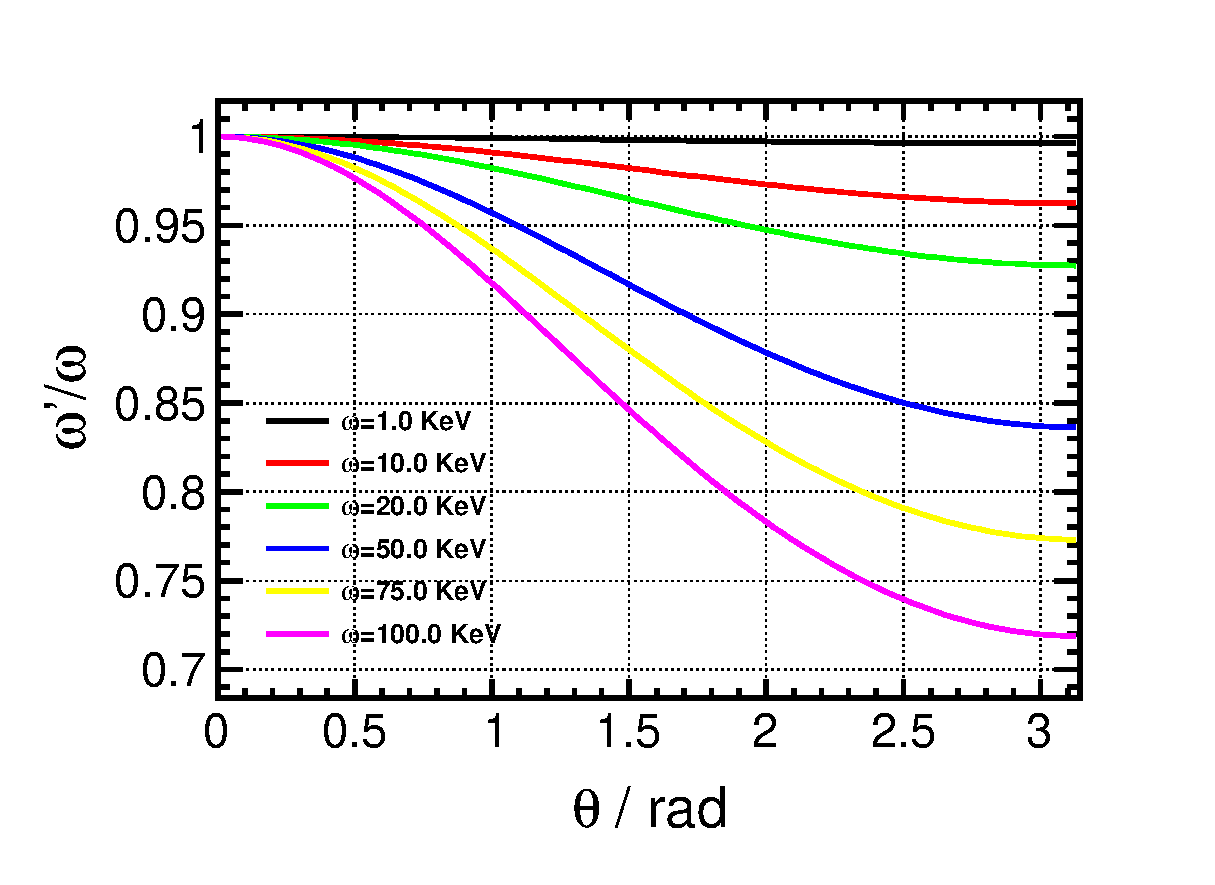
\includegraphics[width=0.85\textwidth]{Compton.eps}
    \caption{\label{fig:Compton} Distribution of energy of outgoing photons with respect to scatter angle. Lines with different colors represent different energies incoming photons have.}
    \end{figure}
    \item If mass of electron is zero, the scattering angle $\theta$ must be zero to vanish the diverging term in the denominator, otherwise the $\omega'$ would be zero which is impossible for photons. It leads $\omega'$ to be the same as $\omega$. Therefore, the incoming photon will have no interaction with the electrons. 
    \item In classical theory, electrons will absorb the photon and emit it into different direction with the same energy, thus the distribution of $\omega'$ with respect to $\theta$ will be a uniform distribution.
\end{enumerate}
\end{solution}

\begin{problem}
(Schwartz 2.6) Lorentz invariance.
\begin{enumerate}[(a)]
    \item Show that
    \begin{equation}
        \int^{\infty}_{-\infty}\dd k^0\delta(k^2-m^2)\theta(k^0)=\frac{1}{2\omega_k},
    \end{equation}
    where $\theta(x)$ is the unit step function and $\omega_k\equiv\sqrt{\mathbf{k}^2+m^2}$.
    \item Show that the integration measure $\dd^4 k$ is Lorentz invariant.
    \item Finally, show that
    \begin{equation}
        \int\frac{\dd^3k}{2\omega_k}
    \end{equation}
    is Lorentz invariant.
\end{enumerate}
\end{problem}

\begin{solution}
\begin{enumerate}[(a)]
    \item \begin{align}
        \int_{-\infty}^{+\infty}\dd k^0\delta(k^2-m^2)\theta(k^0)&=\int_{-\infty}^{+\infty}\dd k^0\delta[(k^0-\omega_{k})(k^0+\omega_{k})]\theta(k^0) \nonumber \\
        &=\int_{-\infty}^{+\infty}\dd k^0\frac{\delta(k^0-\omega_{k})+\delta(k^0+\omega_{k})}{2\omega_k}\theta(k^0) \nonumber \\
        &=\frac{1}{2\omega_k}.
    \end{align}
    \item The transformation of the integral measure satisfies the following formula:
    \begin{equation}
        \dd ^4k'=\dd^4k\bigg|\frac{\partial(k'^0, k'^1, k'^2, k'^3)}{\partial(k^0, k^1, k^2, k^3)}\bigg|=\dd^4k |{\rm det}(\Lambda)|=\dd^4k,
    \end{equation}
    where we have used ${\rm det}(\Lambda)=\pm 1$.
    \item \begin{equation}
        \int\frac{\dd^3k}{2\omega_k}=\int\dd^4k\delta(k^2-m^2)\theta(k^0),
    \end{equation}
    because Lorentz Transformation doesn't change the sign of $k^0$ and $\theta(k^0)$ is a Lorentz invariant. Therefore, $\int\frac{\dd^3k}{2\omega_k}$ is a Lorentz invariant.
\end{enumerate}
\end{solution}

\chapter{Klein-Gordon Field}

\begin{problem}
(Peskin 2.1) Classical electromagnetism (with no sources) follows from the action
\begin{equation}
    S=\int\dd^4 x(-\frac{1}{4}F_{\mu\nu}F^{\mu\nu}),
\end{equation}
where $F_{\mu\nu}=\partial_{\mu}A_{\nu}-\partial_{\nu}A_{\mu}$.
\begin{enumerate}[(a)]
    \item Derive Maxwell's equations as the Euler-Lagrange equations of this action, treating the components $A_{\mu}(x)$ as the dynamical variables. Write the equations in standard form by identifying $E^{i}=-F^{0i}$ and $\epsilon^{ijk}B^{k}=-F^{ij}$.
    \item Construct the energy-momentum tensor for this theory. Note that the usual procedure does not result in a symmetric tensor. To remedy that, we can add to $T_{\mu\nu}$ a term of the form $\partial_{\lambda}K^{\lambda\mu\nu}$, where $K^{\lambda\mu\nu}$ is anti-symmetric in its first two indices. Such an object is automatically divergenceless, so
    \begin{equation}
        \hat{T}^{\mu\nu}=T^{\mu\nu}+\partial_{\lambda}K^{\lambda\mu\nu}
    \end{equation}
    is an equally good energy-momentum tensor with the same globally conserved energy and momentum. Show that this construction, with
    \begin{equation}
        K^{\lambda\mu\nu}=F^{\mu\lambda}A^{\nu},
    \end{equation}
    leads to an energy-momentum tensor $\hat{T}$ that is symmetric and yields the standard formulae for the electromagnetic energy and momentum densities:
    \begin{equation}
        \mathcal{E}=\frac{1}{2}(E^2+B^2);\quad\mathbf{S}=\mathbf{E}\times\mathbf{B}
    \end{equation}
\end{enumerate}
\end{problem}

\begin{solution}
\begin{enumerate}[(a)]
    \item Lagrangian of free electromagenetism is
    \begin{equation}
        \mathcal{L}=-\frac{1}{4}F_{\mu\nu}F^{\mu\nu}.
    \end{equation}
    Due to the anti-symmetric of $F_{\mu\nu}$, we have
    \begin{equation}
        F_{\mu\nu}\partial^{\nu}A^{\mu}=-F_{\nu\mu}\partial^{\nu}A^{\mu}=-F_{\mu\nu}\partial^{\mu}A^{\nu},
    \end{equation}
    thus the Lagrangian can be written as
    \begin{equation}
        \mathcal{L}=-\frac{1}{2}(\partial_{\mu}A_{\nu}\partial^{\mu}A^{\nu}-\partial_{\nu}A_{\mu}\partial^{\mu}A^{\nu}).
    \end{equation}
    Take it into Euler-Lagrange equation, to be more clearly, we replace the indices ($\mu, \nu$) in Lagrangian with ($\rho, \sigma$).
    \begin{align}
        0&=\partial_{\mu}\frac{\partial\mathcal{L}}{\partial(\partial_{\mu}A_{\nu})}-\frac{\partial\mathcal{L}}{\partial A_{\nu}} \nonumber \\
        &=-\frac{1}{2}\partial_{\mu}\frac{\partial(\partial_{\rho}A_{\sigma}\partial^{\rho}A^{\sigma}-\partial_{\sigma}A_{\rho}\partial^{\rho}A^{\sigma})}{\partial(\partial_{\mu}A_{\nu})},
    \end{align}
    after a simple indices calculation, we have
    \begin{equation}
        -\frac{1}{2}\partial_{\mu}(\delta_{\rho}^{\mu}\delta_{\sigma}^{\nu}\partial^{\rho}A^{\sigma}+\partial_{\rho}A_{\sigma}g^{\rho\mu}g^{\sigma\nu}-\delta_{\sigma}^{\mu}\delta_{\rho}^{\nu}\partial^{\rho}A^{\sigma}-\partial_{\sigma}A_{\rho}g^{\rho\mu}g^{\sigma\nu})=0.
    \end{equation}
    Finally, we obtain
    \begin{equation}
        \partial_{\mu}F^{\mu\nu}=0,
    \end{equation}
    let $\nu=0$, it turns into
    \begin{equation}
        \partial_{i}F^{i0}=0,
    \end{equation}
    that is
    \begin{equation}
        \nabla\cdot\mathbf{E}=0.
    \end{equation}
    Let $\nu=j=1,2,3$, it becomes
    \begin{equation}
        \partial_{\mu}F^{\mu j}=\partial_{0}F^{0j}+\partial_{i}F^{ij},\label{Eq:magTensor}
    \end{equation}
    take the $\epsilon^{ijk}B^{k}=-F^{ij}$ into Eq. \eqref{Eq:magTensor}, we finally get another Maxwell's equation
    \begin{equation}
        \nabla\times\mathbf{B}=\frac{\partial\mathbf{E}}{\partial t}.
    \end{equation}
    \item The energy-momentum tensor is expressed as 
    \begin{equation}
        T^{\mu\nu}=\frac{\partial\mathcal{L}}{\partial(\partial_{\mu}\phi)}\partial^{\nu}\phi-\mathcal{L}g^{\mu\nu},
    \end{equation}
    take Lagrangian of electromagnetism into it, we have
    \begin{equation}
        T^{\mu\nu}=\frac{1}{4}g^{\mu\nu}F_{\rho\sigma}F^{\rho\sigma}-F^{\mu\lambda}\partial^{\nu}A_{\lambda}.
    \end{equation}
    This quantity is not symmetric while exchanging indices ($\mu, \nu$), however, it's possible to make it symmetric if we add a divergenceless term
    \begin{align}
        \hat{T}^{\mu\nu}&=T^{\mu\nu}+\partial_{\lambda}K^{\lambda\mu\nu} \nonumber \\
        &=\frac{1}{4}g^{\mu\nu}F_{\rho\sigma}F^{\rho\sigma}+F^{\mu\lambda}F_{\lambda}^{\enspace\nu},
    \end{align}
    where we have used $\partial_{\mu}F^{\mu\nu}=0$. We can show that the last term is symmetric under exchanging ($\mu, \nu$):
    \begin{equation}
        F^{\nu\lambda}F_{\lambda}^{\enspace\mu}=F^{\nu\lambda}F^{\rho\mu}g_{\rho\lambda}=F^{\nu\rho}F^{\lambda\mu}g_{\rho\lambda}=F^{\lambda\mu}F_{\enspace\lambda}^{\nu}=F^{\mu\lambda}F_{\lambda}^{\enspace\nu},
    \end{equation}
    therefore, the new energy-momentum tensor $\hat{T}^{\mu\nu}$ is symmetric. \\
    The $\hat{T}^{00}$ gives energy density of electromagnetic
    \begin{align}
        \hat{T}^{00}=\mathcal{E}=&=\frac{1}{4}F_{\rho\sigma}F^{\rho\sigma}+F^{0\lambda}F_{\lambda}^{\enspace 0} \nonumber \\
        &=\frac{1}{4}(F_{0\sigma}F^{0\sigma}+F_{i\sigma}F^{i\sigma})+F^{0i}F_{i}^{\enspace 0} \nonumber \\
        &=\frac{1}{4}(F_{0i}F^{0i}+F_{i0}F^{i0}+F_{ij}F^{ij})+F^{0i}F_{i}^{\enspace 0} \nonumber \\
        &=\frac{1}{2}(\mathbf{E}^2+\mathbf{B}^2).
    \end{align}
    The $\hat{T}^{0i}$ gives momentum density of electromagnetic
    \begin{align}
        \hat{T}^{0i}=S^i=&=F^{0\lambda}F_{\lambda}^{\enspace i}=F^{0j}F_{j}^{\enspace i} \nonumber \\
        &=(-E^{j})(\epsilon^{jik}B^{k}) \nonumber \\
        &=\epsilon^{ijk}E^{j}B^{k}\ ,
    \end{align}
    in vector form, it is
    \begin{align}
        \mathbf{S}=\mathbf{E}\times\mathbf{B}.
    \end{align}
\end{enumerate}
\end{solution}

\begin{problem}\label{Prob2.2}
(Peskin 2.2) The complex scalar field. Consider the field theory of a complex-valued scalar field obeying the Klein-Gordon equation. The action of this theory is
\begin{equation}
    S=\int\dd^4 x(\partial_{\mu}\phi^{*}\partial^{\mu}\phi-m^2\phi^{*}\phi).
\end{equation}
It is easiest to analyse this theory by considering $\phi(x)$ and $\phi^{*}(x)$, rather than the real and imaginary parts of $\phi(x)$, as the basic dynamical variables.
\begin{enumerate}[(a)]
    \item Find the conjugate momenta to $\phi(x)$ and $\phi^{*}(x)$ and the canonical commutation relations. Show that the Hamiltonian is
    \begin{equation}
        H=\int\dd^3 x(\pi^{*}\pi+\nabla\phi^{*}\cdot\nabla\phi+m^2\phi^*\phi).
    \end{equation}
    Compute the Heisenberg equation of motion for $\phi(x)$ and show that it is indeed the Klein-Gordon equation.
    \item Diagonalize $H$ by introducing creation and annihilation operators. Show that the theory contains two set of particles of mass $m$.
    \item Rewrite the conserved charge
    \begin{equation}
        Q=i\int\dd^3 x(\phi^*\pi^*-\pi\phi) \label{Eq:unGeneralized Q}
    \end{equation}
    in terms of creation and annihilation operators, and evaluate the charge of particle of each type.
    \item Consider the case of two complex Klein-Gordon fields with the same mass. Label the fields as $\phi_{a}(x)$, where $a=1,2$. Show that there are now four conserved charges, one given by the generalization of part (c), and the other three given by
    \begin{equation}
        Q^{i}=\int\dd^3 x\frac{i}{2}\Big(\phi^{*}_{a}(\sigma^{i})_{ab}\pi^{*}_{b}-\pi_{a}(\sigma^{i})_{ab}\phi_{b}\Big),
    \end{equation}
    where $\sigma^{i}$ are the Pauli sigma matrices. Show that these three charges have the commutation relations of angular momentum ($\mathrm{SU(2)}$). Generalize these results to the case of $n$ identical complex scalar fields.
\end{enumerate}
\end{problem}

\begin{solution}
\begin{enumerate}[(a)]
    \item The conjugate momentum has the form
    \begin{equation}
        \pi(x)=\frac{\partial\mathcal{L}}{\partial\dot{\phi}(x)},
    \end{equation}
    which gives $\pi (x)$ and $\pi^*(x)$
    \begin{align}
        \pi(x)&=\dot{\phi}^*(x), \label{Eq:canonical momentum1}\\
        \pi^*(x)&=\dot{\phi}(x). \label{Eq:canonical momentum2}
    \end{align}
    The canonical commutation relations are given by the canonical quantization condition
    \begin{equation}
        [\phi(\mathbf{x},t),\pi(\mathbf{y},t)]=[\phi^*(\mathbf{x},t),\pi^*(\mathbf{y},t)]=i\delta^{3}(\mathbf{x-y}). \label{Eq:commutator}
    \end{equation}
    The Hamiltonian 
    \begin{align}
        H&=\int\dd^3 x(\pi_{i}\dot{\phi}^{i}-\mathcal{L}) \nonumber \\
        &=\int\dd^3 x(\partial_{0}\phi^{*}\partial^{0}\phi+\partial_{0}\phi\partial^{0}\phi^{*}-\mathcal{L}) \nonumber \\
        &=\int\dd^3 x(\partial_{0}\phi\partial^{0}\phi^{*}+\nabla\phi^{*}\cdot\nabla\phi+m^{2}\phi^{*}\phi) \nonumber \\
        &=\int\dd^3 x(\pi^{*}\pi+\nabla\phi^{*}\cdot\nabla\phi+m^2\phi^*\phi).
    \end{align}
    Take $\pi$ and $\pi^{*}$ into the Heisenberg equation
    \begin{align}
        i\frac{\partial\pi}{\partial t}&=[\pi,H]=i(\nabla^2-m^2)\phi^{*}, \\
        i\frac{\partial\pi^{*}}{\partial t}&=[\pi^{*},H]=i(\nabla^2-m^2)\phi,
    \end{align}
    notice that $\nabla\phi^{*}\cdot\nabla\phi = \nabla(\phi^{*}\nabla\phi)-\phi^{*}\nabla^2\phi = \nabla(\phi\nabla\phi^{*})-\phi\nabla^2\phi^{*}$, and the three-divergence term is vanished after the full space integral. \\
    Take Eq. \eqref{Eq:canonical momentum1} and Eq. \eqref{Eq:canonical momentum2} into above formulae, we have
    \begin{align}
        (\partial^2+m^2)\phi(x)&=0, \\
        (\partial^2+m^2)\phi^{*}(x)&=0,
    \end{align}
    which shows that $\phi(x)$ and $\phi^{*}(x)$ both satisfy the Klein-Gordon equation.
    \item As same as the real Klein-Gordon field, we expand the complex field in plane wave formulation
    \begin{align}
        \phi(x)&=\int\frac{\dd^3\mathbf{p}}{(2\pi)^3}\frac{1}{\sqrt{2E_{\mathbf{p}}}}(a_{\mathbf{p}}e^{-ipx}+b_{\mathbf{p}}e^{ipx}), \\
        \phi^{\dagger}(x)&=\int\frac{\dd^3\mathbf{p}}{(2\pi)^3}\frac{1}{\sqrt{2E_{\mathbf{p}}}}(a^{\dagger}_{\mathbf{p}}e^{ipx}+b^{\dagger}_{\mathbf{p}}e^{-ipx}), \\
        \pi(x)&=\int\frac{\dd^3\mathbf{p}}{(2\pi)^3}i\sqrt{\frac{E_{\mathbf{p}}}{2}}(a^{\dagger}_{\mathbf{p}}e^{ipx}-b^{\dagger}_{\mathbf{p}}e^{-ipx}), \\
        \pi^{\dagger}(x)&=\int\frac{\dd^3\mathbf{p}}{(2\pi)^3}(-i)\sqrt{\frac{E_{\mathbf{p}}}{2}}(a_{\mathbf{p}}e^{-ipx}-b_{\mathbf{p}}e^{ipx}),
    \end{align}
    assuming the commutation relationships of $a_{\mathbf{p}}$ and $b_{\mathbf{p}}$
    \begin{equation}
        [a_{\mathbf{p}},a^{\dagger}_{\mathbf{q}}]=[b_{\mathbf{p}},b^{\dagger}_{\mathbf{q}}]=(2\pi)^3\delta^3(\mathbf{p-q}),
    \end{equation}
    we can calculate the commutator of $\phi$ and $\pi$
    \begin{align}
        [\phi(\mathbf{x},t),\pi(\mathbf{y},t)]&=\int\frac{\dd^3\mathbf{p}\dd^3\mathbf{q}}{(2\pi)^6}(\frac{i}{2})\sqrt{\frac{E_{\mathbf{q}}}{E_{\mathbf{p}}}}\Big([a_{\mathbf{p}},a^{\dagger}_{q}]e^{-i(px-qy)}-[b_{\mathbf{p}},b^{\dagger}_{q}]e^{i(px-qy)}\Big) \nonumber \\
        &=\int\frac{\dd^3\mathbf{p}\dd^3\mathbf{q}}{(2\pi)^6}(\frac{i}{2})\sqrt{\frac{E_{\mathbf{q}}}{E_{\mathbf{p}}}}(2\pi)^3\delta^3(\mathbf{p-q})\Big(e^{-i(px-qy)}-e^{i(px-qy)}\Big) \nonumber \\
        &=\int\frac{\dd^3\mathbf{p}}{(2\pi)^3}(\frac{i}{2})\Big(e^{i\mathbf{p}\cdot(\mathbf{x-y})}-e^{-i\mathbf{p}\cdot(\mathbf{x-y})}\Big) \nonumber \\
        &=0,
    \end{align}
    which is different from Eq. \eqref{Eq:commutator}. To obtain the correct time-equal canonical commutation relationship, the simplest way is exchanging the position of $b_{\mathbf{p}}$ and $b_{\mathbf{p}}^{\dagger}$ in $\phi$ and $\pi$, that is
    \begin{align}
        \phi(x)&=\int\frac{\dd^3\mathbf{p}}{(2\pi)^3}\frac{1}{\sqrt{2E_{\mathbf{p}}}}\Big(a_{\mathbf{p}}e^{-ipx}+b^{\dagger}_{\mathbf{p}}e^{ipx}\Big), \\
        \phi^{\dagger}(x)&=\int\frac{\dd^3\mathbf{p}}{(2\pi)^3}\frac{1}{\sqrt{2E_{\mathbf{p}}}}\Big(a^{\dagger}_{\mathbf{p}}e^{ipx}+b_{\mathbf{p}}e^{-ipx}\Big), \\
        \pi(x)&=\int\frac{\dd^3\mathbf{p}}{(2\pi)^3}i\sqrt{\frac{E_{\mathbf{p}}}{2}}\Big(a^{\dagger}_{\mathbf{p}}e^{ipx}-b_{\mathbf{p}}e^{-ipx}\Big), \\
        \pi^{\dagger}(x)&=\int\frac{\dd^3\mathbf{p}}{(2\pi)^3}(-i)\sqrt{\frac{E_{\mathbf{p}}}{2}}\Big(a_{\mathbf{p}}e^{-ipx}-b^{\dagger}_{\mathbf{p}}e^{ipx}\Big),
    \end{align}
    From the proper expansion of field operator, we can obtain the correct commutation relationships. 
    \begin{align}
        [\phi(\mathbf{x},t),\pi(\mathbf{y},t)]&=\int\frac{\dd^3\mathbf{p}\dd^3\mathbf{q}}{(2\pi)^6}(\frac{i}{2})\sqrt{\frac{E_{\mathbf{q}}}{E_{\mathbf{p}}}}\Big([a_{\mathbf{p}},a^{\dagger}_{q}]e^{-i(px-qy)}-[b^{\dagger}_{\mathbf{p}},b_{q}]e^{i(px-qy)}\Big) \nonumber \\
        &=\int\frac{\dd^3\mathbf{p}\dd^3\mathbf{q}}{(2\pi)^6}(\frac{i}{2})\sqrt{\frac{E_{\mathbf{q}}}{E_{\mathbf{p}}}}(2\pi)^3\delta^3(\mathbf{p-q})\Big(e^{-i(px-qy)}+e^{i(px-qy)}\Big) \nonumber \\
        &=\int\frac{\dd^3\mathbf{p}}{(2\pi)^3}(\frac{i}{2})\Big(e^{i\mathbf{p}\cdot(\mathbf{x-y})}+e^{-i\mathbf{p}\cdot(\mathbf{x-y})}\Big) \nonumber \\
        &=i\delta^3(\mathbf{x-y}),
    \end{align}
    commutator of $\phi^{\dagger}$ and $\pi^{\dagger}$ is correct after the same process as well
    \begin{align}
        [\phi^{\dagger}(\mathbf{x},t),\pi^{\dagger}(\mathbf{y},t)]&=\int\frac{\dd^3\mathbf{p}\dd^3\mathbf{q}}{(2\pi)^6}(-\frac{i}{2})\sqrt{\frac{E_{\mathbf{q}}}{E_{\mathbf{p}}}}\Big([a^{\dagger}_{\mathbf{p}},a_{q}]e^{i(px-qy)}-[b_{\mathbf{p}},b^{\dagger}_{q}]e^{-i(px-qy)}\Big) \nonumber \\
        &=\int\frac{\dd^3\mathbf{p}\dd^3\mathbf{q}}{(2\pi)^6}(\frac{i}{2})\sqrt{\frac{E_{\mathbf{q}}}{E_{\mathbf{p}}}}(2\pi)^3\delta^3(\mathbf{p-q})\Big(e^{i(px-qy)}+e^{-i(px-qy)}\Big) \nonumber \\
        &=\int\frac{\dd^3\mathbf{p}}{(2\pi)^3}(\frac{i}{2})\Big(e^{-i\mathbf{p}\cdot(\mathbf{x-y})}+e^{i\mathbf{p}\cdot(\mathbf{x-y})}\Big) \nonumber \\
        &=i\delta^3(\mathbf{x-y}).
    \end{align}
    Substituting the $\phi_{i}$ and $\pi_{i}$ with Fourier series in Hamiltonian, we can diagonalize it
    \begin{align*}
        H&=\int\dd^3 x(\pi^{\dagger}\pi+\nabla\phi^{\dagger}\cdot\nabla\phi+m^2\phi^{\dagger}\phi) \\
        &=\int\dd^3 x\int\frac{\dd^3\mathbf{p}}{(2\pi)^3}\frac{1}{\sqrt{2E_{\mathbf{p}}}}\frac{\dd^3\mathbf{q}}{(2\pi)^3}\frac{1}{\sqrt{2E_{\mathbf{q}}}} \\
        &\quad\times
        \Bigg[E_{\mathbf{p}}E_{\mathbf{q}}\Big(a^{\dagger}_{\mathbf{p}}e^{ipx}-b_{\mathbf{p}}e^{-ipx}\Big)\Big(a_{\mathbf{q}}e^{-iqx}-b^{\dagger}_{\mathbf{q}}e^{iqx}\Big) \\
        &\quad\quad+\mathbf{p\cdot q}\Big(a^{\dagger}_{\mathbf{p}}e^{ipx}-b_{\mathbf{p}}e^{-ipx}\Big)\Big(a_{\mathbf{q}}e^{-iqx}-b^{\dagger}_{\mathbf{q}}e^{iqx}\Big) \\
        &\quad\quad+m^2\Big(a^{\dagger}_{\mathbf{p}}e^{ipx}+b_{\mathbf{p}}e^{-ipx}\Big)\Big(a_{\mathbf{q}}e^{-iqx}+b^{\dagger}_{\mathbf{q}}e^{iqx}\Big)
        \Bigg] \\
        &=\int\dd^3 x\int\frac{\dd^3\mathbf{p}}{(2\pi)^3}\frac{1}{\sqrt{2E_{\mathbf{p}}}}\frac{\dd^3\mathbf{q}}{(2\pi)^3}\frac{1}{\sqrt{2E_{\mathbf{q}}}} \\
        &\quad\times\Bigg[(E_{\mathbf{p}}E_{\mathbf{q}}+\mathbf{p\cdot q}+m^2)\Big(a^{\dagger}_{\mathbf{p}}a_{\mathbf{q}}e^{i(p-q)x}+b_{\mathbf{p}}b^{\dagger}_{\mathbf{q}}e^{-i(p-q)x}\Big) \\
        &\quad\quad-(E_{\mathbf{p}}E_{\mathbf{q}}+\mathbf{p\cdot q}-m^2)\Big(a^{\dagger}_{\mathbf{p}}b^{\dagger}_{\mathbf{q}}e^{i(p+q)x}+b_{\mathbf{p}}a_{\mathbf{q}}e^{-i(p+q)x}\Big)
        \Bigg] \\
        &=\int\frac{\dd^3\mathbf{p}}{(2\pi)^3}\frac{1}{\sqrt{2E_{\mathbf{p}}}}\frac{\dd^3\mathbf{q}}{(2\pi)^3}\frac{1}{\sqrt{2E_{\mathbf{q}}}} \\
        &\quad\times\Bigg[(E_{\mathbf{p}}E_{\mathbf{q}}+\mathbf{p\cdot q}+m^2)\Big(a^{\dagger}_{\mathbf{p}}a_{\mathbf{q}}e^{i(E_{\mathbf{p}}-E_{\mathbf{q}})t}+b_{\mathbf{p}}b^{\dagger}_{\mathbf{q}}e^{-i(E_{\mathbf{p}}-E_{\mathbf{q}})t}\Big)(2\pi)^3\delta^3(\mathbf{p-q}) \\
        &\quad\quad-(E_{\mathbf{p}}E_{\mathbf{q}}+\mathbf{p\cdot q}-m^2)\Big(a^{\dagger}_{\mathbf{p}}b^{\dagger}_{\mathbf{q}}e^{i(E_{\mathbf{p}}+E_{\mathbf{q}})t}+b_{\mathbf{p}}a_{\mathbf{q}}e^{-i(E_{\mathbf{p}}+E_{\mathbf{q}})t}\Big)(2\pi)^3\delta^3(\mathbf{p+q})
        \Bigg] \\
        &=\int\frac{\dd^3\mathbf{p}}{(2\pi)^3}\frac{1}{2E_{\mathbf{p}}}\times
        (E^2_{\mathbf{p}}+\mathbf{p}^2+m^2)\Big(a^{\dagger}_{\mathbf{p}}a_{\mathbf{p}}+b_{\mathbf{p}}b^{\dagger}_{\mathbf{p}}\Big) \\
        &=\int\frac{\dd^3\mathbf{p}}{(2\pi)^3}E_{\mathbf{p}}\Big(a^{\dagger}_{\mathbf{p}}a_{\mathbf{p}}+b^{\dagger}_{\mathbf{p}}b_{\mathbf{p}}+(2\pi)^3\delta^3(\mathbf{0})\Big).
    \end{align*}
    The infinite term is not observable thus we can easily drop it, therefore, the Hamiltonian is
    \begin{equation}
        H=\int\frac{\dd^3\mathbf{p}}{(2\pi)^3}E_{\mathbf{p}}\Big(a^{\dagger}_{\mathbf{p}}a_{\mathbf{p}}+b^{\dagger}_{\mathbf{p}}b_{\mathbf{p}}\Big).
    \end{equation}
    Momentum operator can also be calculate by following equation
    \begin{align*}
        \mathbf{P}&=T^{0i}=\frac{\partial\mathcal{L}}{\partial(\partial_{0}\phi)}\partial^{i}\phi-\mathcal{L}g^{0i}=-\pi\partial_{i}\phi \\
        &=\int\dd^3x\int\frac{\dd^3\mathbf{p}}{(2\pi)^3}\frac{1}{\sqrt{2E_{\mathbf{p}}}}\frac{\dd^3\mathbf{q}}{(2\pi)^3}\frac{1}{\sqrt{2E_{\mathbf{q}}}} \\
        &\quad\times\Big[E_{\mathbf{p}}\mathbf{q}\Big(a^{\dagger}_{\mathbf{p}}e^{ipx}-b_{\mathbf{p}}e^{-ipx}\Big)\Big(a_{\mathbf{q}}e^{-iqx}-b^{\dagger}_{\mathbf{q}}e^{iqx}\Big) \\
        &\quad\quad+E_{\mathbf{q}}\mathbf{p}\Big(a^{\dagger}_{\mathbf{p}}e^{ipx}-b_{\mathbf{p}}e^{-ipx}\Big)\Big(a_{\mathbf{q}}e^{-iqx}-b^{\dagger}_{\mathbf{q}}e^{iqx}\Big)
        \Big] \\
        &=\int\dd^3x\int\frac{\dd^3\mathbf{p}}{(2\pi)^3}\frac{1}{\sqrt{2E_{\mathbf{p}}}}\frac{\dd^3\mathbf{q}}{(2\pi)^3}\frac{1}{\sqrt{2E_{\mathbf{q}}}} \\
        &\quad\times\Big[(E_{\mathbf{p}}\mathbf{q}+E_{\mathbf{q}}\mathbf{p})\Big(a^{\dagger}_{\mathbf{p}}a_{\mathbf{q}}e^{i(p-q)x}+b_{\mathbf{p}}b^{\dagger}_{\mathbf{q}}e^{-i(p-q)x}\Big) \\
        &\quad\quad-(E_{\mathbf{p}}\mathbf{q}+E_{\mathbf{q}}\mathbf{p})\Big(a^{\dagger}_{\mathbf{p}}b^{\dagger}_{\mathbf{q}}e^{i(p+q)x}+b_{\mathbf{p}}a_{\mathbf{q}}e^{-i(p+q)x}\Big) 
        \Big] \\
        &=\int\frac{\dd^3\mathbf{p}}{(2\pi)^3}\frac{1}{\sqrt{2E_{\mathbf{p}}}}\frac{\dd^3\mathbf{q}}{(2\pi)^3}\frac{1}{\sqrt{2E_{\mathbf{q}}}} \\
        &\quad\times\Big[(E_{\mathbf{p}}\mathbf{q}+E_{\mathbf{q}}\mathbf{p})\Big(a^{\dagger}_{\mathbf{p}}a_{\mathbf{q}}e^{i(E_{\mathbf{p}}-E_{\mathbf{q}})t}+b_{\mathbf{p}}b^{\dagger}_{\mathbf{q}}e^{-i(E_{\mathbf{p}}-E_{\mathbf{q}})t}\Big)(2\pi)^3\delta^3(\mathbf{p-q}) \\
        &\quad\quad-(E_{\mathbf{p}}\mathbf{q}+E_{\mathbf{q}}\mathbf{p})\Big(a^{\dagger}_{\mathbf{p}}b^{\dagger}_{\mathbf{q}}e^{i(E_{\mathbf{p}}+E_{\mathbf{q}})t}+b_{\mathbf{p}}a_{\mathbf{q}}e^{-i(E_{\mathbf{p}}+E_{\mathbf{q}})t}\Big)(2\pi)^3\delta^3(\mathbf{p+q}) 
        \Big] \\
        &=\int\frac{\dd^3\mathbf{p}}{(2\pi)^3}\mathbf{p}\Big(a^{\dagger}_{\mathbf{p}}a_{\mathbf{p}}+b_{\mathbf{p}}b^{\dagger}_{\mathbf{p}}\Big) \\
        &=\int\frac{\dd^3\mathbf{p}}{(2\pi)^3}\mathbf{p}\Big(a^{\dagger}_{\mathbf{p}}a_{\mathbf{p}}+b^{\dagger}_{\mathbf{p}}b_{\mathbf{p}}\Big)+\int\dd^3\mathbf{p}\delta^3(\mathbf{0})\mathbf{p} \\
        &=\int\frac{\dd^3\mathbf{p}}{(2\pi)^3}\mathbf{p}\Big(a^{\dagger}_{\mathbf{p}}a_{\mathbf{p}}+b^{\dagger}_{\mathbf{p}}b_{\mathbf{p}}\Big),
    \end{align*}
    therefore the momentum operator is
    \begin{equation}
        \mathbf{P}=\int\frac{\dd^3\mathbf{p}}{(2\pi)^3}\mathbf{p}\Big(a^{\dagger}_{\mathbf{p}}a_{\mathbf{p}}+b^{\dagger}_{\mathbf{p}}b_{\mathbf{p}}\Big).
    \end{equation}
    The commutation relationships between $P=(H,\mathbf{P})$ and $a^{(\dagger)}_{\mathbf{p}}$ as well as $b^{(\dagger)}_{\mathbf{p}}$ is easy to derive
    \begin{align}
        [H,a_{\mathbf{p}}]&=-E_{\mathbf{p}}a_{\mathbf{p}},\quad[H,b_{\mathbf{p}}]=-E_{\mathbf{p}}b_{\mathbf{p}}, \\
        [H,a^{\dagger}_{\mathbf{p}}]&=+E_{\mathbf{p}}a^{\dagger}_{\mathbf{p}},\quad[H,b^{\dagger}_{\mathbf{p}}]=+E_{\mathbf{p}}b^{\dagger}_{\mathbf{p}}, \\
        [\mathbf{P},a_{\mathbf{p}}]&=-\mathbf{p}a_{\mathbf{p}},\quad\enspace[\mathbf{P},b_{\mathbf{p}}]=-\mathbf{p}b_{\mathbf{p}}, \\
        [\mathbf{P},a^{\dagger}_{\mathbf{p}}]&=+\mathbf{p}a^{\dagger}_{\mathbf{p}},\quad\enspace[\mathbf{P},b^{\dagger}_{\mathbf{p}}]=+\mathbf{p}b^{\dagger}_{\mathbf{p}}.
    \end{align}
    To examine the functionality of $a^{(\dagger)}_{\mathbf{p}}$ and $b^{(\dagger)}_{\mathbf{p}}$, let $|\Psi_{0}\rangle$ to be the eigen-state of $P$ operator
    \begin{equation}
        H|\Psi_{0}\rangle=E_{0}|\Psi_{0}\rangle,\quad\mathbf{P}|\Psi_{0}\rangle=\mathbf{p}_{0}|\Psi_{0}\rangle,
    \end{equation}
    for the $a_{\mathbf{p}}|\Psi_{0}\rangle$, we have
    \begin{equation}
        Ha_{\mathbf{p}}|\Psi_{0}\rangle=(a_{\mathbf{p}}H-E_{\mathbf{p}}a_{\mathbf{p}})|\Psi_{0}\rangle=(E_{0}-E_{\mathbf{p}})a_{\mathbf{p}}|\Psi_{0}\rangle,
    \end{equation}
    \begin{equation}
        \mathbf{P}a_{\mathbf{p}}|\Psi_{0}\rangle=(a_{\mathbf{p}}\mathbf{P}-\mathbf{p}a_{\mathbf{p}})|\Psi_{0}\rangle=(\mathbf{p}_{0}-\mathbf{p})a_{\mathbf{p}}|\Psi_{0}\rangle,
    \end{equation}
    for the $a^{\dagger}_{\mathbf{p}}|\Psi_{0}\rangle$, we have
    \begin{equation}
        Ha^{\dagger}_{\mathbf{p}}|\Psi_{0}\rangle=(a^{\dagger}_{\mathbf{p}}H+E_{\mathbf{p}}a^{\dagger}_{\mathbf{p}})|\Psi_{0}\rangle=(E_{0}+E_{\mathbf{p}})a^{\dagger}_{\mathbf{p}}|\Psi_{0}\rangle,
    \end{equation}
    \begin{equation}
        \mathbf{P}a^{\dagger}_{\mathbf{p}}|\Psi_{0}\rangle=(a^{\dagger}_{\mathbf{p}}\mathbf{P}+\mathbf{p}a^{\dagger}_{\mathbf{p}})|\Psi_{0}\rangle=(\mathbf{p}_{0}+\mathbf{p})a^{\dagger}_{\mathbf{p}}|\Psi_{0}\rangle,
    \end{equation}
    the similar results can be obtained by replacing $a^{(\dagger)}_{\mathbf{p}}$ with $b^{(\dagger)}_{\mathbf{p}}$. \\
    We can see that the $a_{\mathbf{p}}$ and $b_{\mathbf{p}}$ annihilate a particle with mass $m$ and four-momentum $p^{\mu}=(E_{\mathbf{p}},\mathbf{p})$, and the $a^{\dagger}_{\mathbf{p}}$ and $b^{\dagger}_{\mathbf{p}}$ create a particle with mass $m$ and four-momentum $p^{\mu}=(E_{\mathbf{p}},\mathbf{p})$, therefore, this quantized complex scalar field theory contains two set of particles of mass $m$.
    \item The conserved charge $Q$ is 
    \begin{align}
        Q&=i\int\dd^3 x(\phi^{\dagger}\pi^{\dagger}-\pi\phi) \nonumber \\
        &=\int\dd^3 x\int\frac{\dd^3\mathbf{p}}{(2\pi)^3}\frac{1}{\sqrt{2E_{\mathbf{p}}}}\frac{\dd^3\mathbf{q}}{(2\pi)^3}\frac{1}{\sqrt{2E_{\mathbf{q}}}} \nonumber \\
        &\quad\times\Big[E_{\mathbf{q}}\Big(a^{\dagger}_{\mathbf{p}}e^{ipx}+b_{\mathbf{p}}e^{-ipx}\Big)\Big(a_{\mathbf{q}}e^{-iqx}-b^{\dagger}_{\mathbf{q}}e^{iqx}\Big) \nonumber \\
        &\quad\quad+E_{\mathbf{p}}\Big(a^{\dagger}_{\mathbf{p}}e^{ipx}-b_{\mathbf{p}}e^{-ipx}\Big)\Big(a_{\mathbf{q}}e^{-iqx}+b^{\dagger}_{\mathbf{q}}e^{iqx}\Big)
        \Big] \nonumber \\
        &=\int\dd^3 x\int\frac{\dd^3\mathbf{p}}{(2\pi)^3}\frac{1}{\sqrt{2E_{\mathbf{p}}}}\frac{\dd^3\mathbf{q}}{(2\pi)^3}\frac{1}{\sqrt{2E_{\mathbf{q}}}} \nonumber \\
        &\quad\times\Bigg[(E_{\mathbf{q}}+E_{\mathbf{p}})\Big(a^{\dagger}_{\mathbf{p}}a_{\mathbf{q}}e^{i(p-q)x}-b_{\mathbf{p}}b^{\dagger}_{\mathbf{q}}e^{-i(p-q)x}\Big) \nonumber \\
        &\quad\quad+(E_{\mathbf{p}}-E_{\mathbf{q}})\Big(a^{\dagger}_{\mathbf{p}}b^{\dagger}_{\mathbf{q}}e^{i(p+q)x}-b_{\mathbf{p}}b_{\mathbf{q}}e^{-i(p+q)x}\Big)
        \Big] \nonumber \\
        &=\int\frac{\dd^3\mathbf{p}}{(2\pi)^3}\frac{1}{\sqrt{2E_{\mathbf{p}}}}\frac{\dd^3\mathbf{q}}{(2\pi)^3}\frac{1}{\sqrt{2E_{\mathbf{q}}}} \nonumber \\
        &\quad\times\Bigg[(E_{\mathbf{q}}+E_{\mathbf{p}})\Big(a^{\dagger}_{\mathbf{p}}a_{\mathbf{q}}e^{i(E_{\mathbf{p}}-E_{\mathbf{q}})t}-b_{\mathbf{p}}b^{\dagger}_{\mathbf{q}}e^{-i(E_{\mathbf{p}}-E_{\mathbf{q}})t}\Big)(2\pi)^3\delta^3(\mathbf{p-q}) \nonumber \\
        &\quad\quad+(E_{\mathbf{p}}-E_{\mathbf{q}})\Big(a^{\dagger}_{\mathbf{p}}b^{\dagger}_{\mathbf{q}}e^{i(E_{\mathbf{p}}+E_{\mathbf{q}})t}-b_{\mathbf{p}}b_{\mathbf{q}}e^{-i(E_{\mathbf{p}}+E_{\mathbf{q}})t}\Big)(2\pi)^3\delta^3(\mathbf{p+q})
        \Big] \nonumber \\
        &=\int\frac{\dd^3\mathbf{p}}{(2\pi)^3}\Big(a^{\dagger}_{\mathbf{p}}a_{\mathbf{p}}-b^{\dagger}_{\mathbf{p}}b_{\mathbf{p}}+(2\pi)^3\delta^3(\mathbf{0})\Big).
    \end{align}
    Use the same trick applied to the Hamiltonian, the infinite term is dropped off, thus we have
    \begin{equation}
        Q=\int\frac{\dd^3\mathbf{p}}{(2\pi)^3}\Big(a^{\dagger}_{\mathbf{p}}a_{\mathbf{p}}-b^{\dagger}_{\mathbf{p}}b_{\mathbf{p}}\Big),
    \end{equation}
    and the commutators
    \begin{equation}
        [Q,a^{\dagger}_{\mathbf{p}}]=a^{\dagger}_{\mathbf{p}},\quad[Q,b^{\dagger}_{\mathbf{p}}]=-b^{\dagger}_{\mathbf{p}},
    \end{equation}
    which mean that $a^{\dagger}_{\mathbf{p}}$ creates a particle with charge $Q=+1$ and $b^{\dagger}_{\mathbf{p}}$ creates a particle with charge $Q=-1$.
    \item The Lagrangian of two complex Klein-Gordon fields with the same mass is written as
    \begin{equation}
        \mathcal{L}=\partial_{\mu}\phi^{\dagger}_{a}\partial^{\mu}\phi_{a}-m^2\phi^{\dagger}_{a}\phi_{a},
    \end{equation}
    to be more clearly, we arrange the $\phi_{a}$ into a two component vector $\Phi$
    \begin{equation}
        \Phi=
        \begin{pmatrix}
            \phi_{1} \\
            \phi_{2}
        \end{pmatrix},
        \Phi^{\dagger}=
        \begin{pmatrix}
            \phi^{\dagger}_{1} \\
            \phi^{\dagger}_{2}
        \end{pmatrix}^{\text{T}},
    \end{equation}
    thus the Lagrangian is
    \begin{equation}
        \mathcal{L}=\partial_{\mu}\Phi^{\dagger}\partial^{\mu}\Phi-m^2\Phi^{\dagger}\Phi.
    \end{equation}
    Evidently, it is an invariant under transformation $\Phi\rightarrow e^{i\alpha}\Phi$ and $\Phi\rightarrow e^{i\frac{\bm{\sigma}}{2}\cdot\bm{\theta}}\Phi$. The conservation current is written as 
    \begin{equation}
        j^{\mu}=\frac{\partial\mathcal{L}}{\partial(\partial_{\mu}\phi)}\delta_{0}\phi+\mathcal{L}\delta x^{\mu}=\frac{\partial\mathcal{L}}{\partial(\partial_{\mu}\phi)}\delta\phi-\Big(\frac{\partial\mathcal{L}}{\partial(\partial_{\mu}\phi)}\partial_{\nu}\phi-\mathcal{L}\delta^{\mu}_{\enspace\nu}\Big)\delta x^{\nu}, \label{Eq:NoetherCurrent}
    \end{equation}
    where the $\delta_{0}\phi=\phi'(x)-\phi(x)$ and $\delta\phi=\phi'(x')-\phi(x)$, the connection between them is
    \begin{equation}
        \delta\phi=\phi'(x')-\phi(x)=\phi'(x)+\partial_{\mu}\phi\delta x^{\mu}-\phi(x)=\delta_{0}\phi+\partial_{\mu}\phi\delta x^{\mu}.
    \end{equation}
    In this case, the difference of $\Phi$ under infinitesimal transformation $\Phi\rightarrow e^{i\alpha}\Phi$ is
    \begin{align}
        \delta_{0}\Phi&=\Phi'(x)-\Phi(x)=e^{i\alpha}\Phi(x)-\Phi \nonumber \\
        &=(1+i\alpha)\Phi(x)-\Phi(x) \nonumber \\
        &=i\alpha\Phi(x),
    \end{align}
    the difference of $\Phi^{\dagger}$ can also be obtained
    \begin{equation}
        \delta_{0}\Phi^{\dagger}=-i\alpha\Phi^{\dagger}(x).
    \end{equation}
    Similarly, the differences caused by the other infinitesimal transformation $\Phi\rightarrow e^{i\frac{\bm{\sigma}}{2}\cdot\bm{\theta}}\Phi$ are
    \begin{equation}
        \delta_{0}\Phi=i\frac{\sigma^{i}}{2}\theta_{i}\Phi(x),\quad\delta_{0}\Phi^{\dagger}=-i\frac{\sigma^{i}}{2}\theta_{i}\Phi^{\dagger}(x).
    \end{equation}
    Next, we are able to calculate the conservation currents and corresponding charge, for the $\Phi\rightarrow e^{i\alpha}\Phi$
    \begin{equation}
        Q=\int\dd^3 xj^{0}=i\int\dd^3 x(\Phi^{\dagger}\Pi^{\dagger}-\Pi\Phi), \label{Eq:Generalized Q0}
    \end{equation}
    the overall sign can be choosen arbitrary, and $\Pi$ is the generalized canonical momentum
    \begin{equation}
        \Pi=
        \begin{pmatrix}
            \pi_{1} \\
            \pi_{2}
        \end{pmatrix}^{\text{T}},
        \Pi^{\dagger}=
        \begin{pmatrix}
            \pi^{\dagger}_{1} \\
            \pi^{\dagger}_{2} 
        \end{pmatrix}.
    \end{equation}
    We can see that Eq. \eqref{Eq:Generalized Q0} has the same form of Eq. \eqref{Eq:unGeneralized Q}. \par
    For $\Phi\rightarrow e^{i\frac{\bm{\sigma}}{2}\cdot\bm{\theta}}\Phi$
    \begin{align}
        Q^{i}&=i\int\dd^3 x\Big(\Phi^{\dagger}(\frac{\sigma^{i}}{2})\Pi^{\dagger}-\Pi(\frac{\sigma^{i}}{2})\Phi\Big) \nonumber \\
        &=i\int\dd^3 x \Big(\Phi^{\dagger}_{a}(\frac{\sigma^{i}}{2})_{ab}\Pi^{\dagger}_{b}-\Pi_{a}(\frac{\sigma^{i}}{2})_{ab}\Phi_{b}\Big),
    \end{align}
    the commutator of $Q^{i}$ is
    \begin{align}
        [Q^{i},Q^{j}]&=i\cdot i\int\dd^3 x\int\dd^3 y \nonumber \\
        &\quad\times\Big[\Big(\Phi^{\dagger}_{a}(\frac{\sigma^{i}}{2})_{ab}\Pi^{\dagger}_{b}-\Pi_{a}(\frac{\sigma^{i}}{2})_{ab}\Phi_{b}\Big),\Big(\Phi^{\dagger}_{c}(\frac{\sigma^{j}}{2})_{cd}\Pi^{\dagger}_{d}-\Pi_{c}(\frac{\sigma^{j}}{2})_{cd}\Phi_{d}\Big)\Big] \nonumber \\
        &=i\cdot i\int\dd^3 x\int\dd^3 y \nonumber \\
        &\quad\times\Bigg\{\Big[\Phi^{\dagger}_{a}(\frac{\sigma^{i}}{2})_{ab}\Pi^{\dagger}_{b},\Phi^{\dagger}_{c}(\frac{\sigma^{j}}{2})_{cd}\Pi^{\dagger}_{d}\Big]+\Big[\Pi_{a}(\frac{\sigma^{i}}{2})_{ab}\Phi_{b},\Pi_{c}(\frac{\sigma^{j}}{2})_{cd}\Phi_{d}\Big] \nonumber \\
        &\quad\quad-\Big[\Phi^{\dagger}_{a}(\frac{\sigma^{i}}{2})_{ab}\Pi^{\dagger}_{b},\Pi_{c}(\frac{\sigma^{j}}{2})_{cd}\Phi_{d}\Big]-\Big[\Pi_{a}(\frac{\sigma^{i}}{2})_{ab}\Phi_{b},\Phi^{\dagger}_{c}(\frac{\sigma^{j}}{2})_{cd}\Pi^{\dagger}_{d}\Big]\Bigg\},
    \end{align}
    the first commutator in the integral is
    \begin{align}
        &\quad\Big[\Phi^{\dagger}_{a}(\frac{\sigma^{i}}{2})_{ab}\Pi^{\dagger}_{b},\Phi^{\dagger}_{c}(\frac{\sigma^{j}}{2})_{cd}\Pi^{\dagger}_{d}\Big] \nonumber \\
        &=
        \Phi^{\dagger}_{a}(\frac{\sigma^{i}}{2})_{ab}\Pi^{\dagger}_{b}\Phi^{\dagger}_{c}(\frac{\sigma^{j}}{2})_{cd}\Pi^{\dagger}_{d}
        -\Phi^{\dagger}_{c}(\frac{\sigma^{j}}{2})_{cd}\Pi^{\dagger}_{d}\Phi^{\dagger}_{a}(\frac{\sigma^{i}}{2})_{ab}\Pi^{\dagger}_{b} \nonumber \\
        &=\Bigg\{\Phi^{\dagger}_{a}(\frac{\sigma^{i}}{2})_{ab}\Big(\Phi^{\dagger}_{c}\Pi^{\dagger}_{b}-i\delta^3(\mathbf{x-y})\delta_{cb}\Big)(\frac{\sigma^{j}}{2})_{cd}\Pi^{\dagger}_{d} -\Phi^{\dagger}_{c}(\frac{\sigma^{j}}{2})_{cd}\Big(\Phi^{\dagger}_{a}\Pi^{\dagger}_{d}-i\delta^3(\mathbf{x-y})\delta_{ad}\Big)(\frac{\sigma^{i}}{2})_{ab}\Pi^{\dagger}_{b}
        \Bigg\} \nonumber \\
        &=-i\delta^3(\mathbf{x-y})\Phi^{\dagger}_{a}\Big[\frac{\sigma^i}{2},\frac{\sigma^j}{2}\Big]_{ab}\Pi^{\dagger}_{b} \nonumber \\
        &=\delta^3(\mathbf{x-y})\epsilon^{ijk}\Phi^{\dagger}_{a}(\frac{\sigma^k}{2})_{ab}\Pi^{\dagger}_{b},
    \end{align}
    finally, we have
    \begin{align}
        [Q^{i},Q^{j}]&=i\epsilon^{ijk}\cdot i\int\dd^3 x\Big(\Phi^{\dagger}_{a}(\frac{\sigma^k}{2})_{ab}\Pi^{\dagger}_{b}-\Pi_{a}(\frac{\sigma^k}{2})_{ab}\Phi_{b}\Big) \nonumber \\
        &=i\epsilon^{ijk}Q^{k},
    \end{align}
    which has the same commutation relations of angular momentum. \par
    Generally, for the case of $n$ identical complex scalar field, the $\Phi$ is
    \begin{equation}
        \Phi=
        \begin{pmatrix}
            \phi_{1} \\
            \phi_{2} \\
            \vdots \\
            \phi_{n}
        \end{pmatrix},
    \end{equation}
    to get the generalized conservation charge, the only thing to do is replacing the $\frac{\sigma^i}{2}$ with $t^{i}$, which is the generator of $\mathrm{SU(n)}$
    \begin{equation}
        Q^{i}=i\int\dd^3 x \Big(\Phi^{\dagger}_{a}t^{i}_{ab}\Pi^{\dagger}_{b}-\Pi_{a}t^{i}_{ab}\Phi_{b}\Big),
    \end{equation}
    and the commutator has similar form
    \begin{equation}
        [Q^{a},Q^{b}]=if^{abc}Q^{c}
    \end{equation}
    where $f^{abc}$ is the structure constant of $\mathfrak{su(n)}$.
\end{enumerate}
\end{solution}

\begin{problem}\label{Prob2.3}
(Peskin 2.3) Evaluate the function
\begin{equation}
    \langle 0|\phi(x)\phi(y)|0\rangle=D(x-y)=\int\frac{\dd^3 p}{(2\pi)^3}\frac{1}{2E_{\mathbf{p}}}e^{-ip\cdot(x-y)},
\end{equation}
for $(x-y)$ space-like so that $(x-y)^2=-r^2$, explicity in terms of Bessel functions.
\end{problem}

\begin{solution}
For space-like $(x-y)$, we are able to take $(x_0-y_0)=0$ and $|\mathbf{x-y}|^2=\mathbf{r}^2$, and other circumstances can be obtained easily by Lorentz transformation. Thus we have
\begin{align}
    D(x-y)&=\int\frac{\dd^3 p}{(2\pi)^3}\frac{1}{2E_{\mathbf{p}}}e^{-ip\cdot(x-y)} \nonumber \\
    &=\int\frac{\dd^3 p}{(2\pi)^3}\frac{1}{2E_{\mathbf{p}}}e^{i\mathbf{p}\cdot\mathbf{(x-y)}} \nonumber \\
    &=\int\frac{\dd p\dd\cos{\theta}\dd\phi}{(2\pi)^3}\frac{p^2}{2\sqrt{p^2+m^2}}e^{ipr\cos{\theta}} \nonumber \\
    &=\frac{-i}{8\pi^2 r}\int_{-\infty}^{+\infty}\dd p\frac{p}{\sqrt{p^2+m^2}}e^{ipr}\ .
\end{align}
Now we replace $p$ with $\rho=-ip$, then the integral becomes
\begin{align}
    D(x-y)&=\frac{1}{4\pi^2r}\int_{m}^{\infty}\dd\rho\frac{\rho}{\sqrt{\rho^2-m^2}}e^{-\rho r} \nonumber \\
    &=\frac{1}{4\pi^2r}\int_{m}^{\infty}\dd\rho \frac{\partial}{\partial\rho}(\sqrt{\rho^2-m^2}) e^{-\rho r} \nonumber \\
    &=\frac{1}{4\pi^2r}\bigg[(\sqrt{\rho^2-m^2}e^{-\rho r})\bigg|_{m}^{\infty}-\int_{m}^{\infty}\dd\rho\sqrt{\rho^2-m^2}\frac{\partial}{\partial\rho}(e^{-\rho r})\bigg] \nonumber \\
    &=\frac{1}{4\pi^2}\int_{m}^{\infty}\dd\rho\sqrt{\rho^2-m^2}e^{-\rho r} \nonumber \\
    &=\frac{m}{4\pi^2r}\mathrm{K}_1(mr)\ ,
\end{align}
where the $\mathrm{K}_1$ is the modified Bessel function
\begin{align}
    \mathrm{K}_{\nu}(z)=\frac{\pi^{\frac{1}{2}}(\frac{1}{2}z)^{\nu}}{\Gamma(\nu+\frac{1}{2})}\int_{1}^{\infty}e^{-zt}(t^2-1)^{\nu-\frac{1}{2}}\dd t\ .
\end{align}
\end{solution}

\begin{problem}
Real Klein-Gordon field theory. Derive to Noether's current and charge of Lorentz transformation. Give the corresponding conservation law of each transformation. 
\end{problem}

\begin{solution}
The Lorentz transformation
\begin{align}
    x^{\mu}\rightarrow x'^{\mu}=\Lambda^{\mu}_{\enspace\nu}x^{\nu}=(\delta^{\mu}_{\enspace\nu}+\omega_{\rho\sigma}(\mathcal{J}^{\rho\sigma})^{\mu}_{\enspace\nu})x^{\nu}\ ,
\end{align}
where $\omega_{\rho\sigma}$ are infinitesimal parameters and $\mathcal{J}^{\rho\sigma}$ are generators of Lorentz transformation, it can be written in $4\times 4$ matrix representation
\begin{align}
    (\mathcal{J}^{\rho\sigma})_{\mu\nu}=(\delta^{\rho}_{\enspace\mu}\delta^{\sigma}_{\enspace\nu}-\delta^{\rho}_{\enspace\nu}\delta^{\sigma}_{\enspace\mu})\ .
\end{align}
The Noether current is commonly written as
\begin{align}
    j^{\mu}=\frac{\partial\mathcal{L}}{\partial(\partial_{\mu}\phi)}\delta_{0}\phi+\mathcal{L}\delta x^{\mu}=\frac{\partial\mathcal{L}}{\partial(\partial_{\mu}\phi)}\delta\phi-\Big(\frac{\partial\mathcal{L}}{\partial(\partial_{\mu}\phi)}\partial_{\nu}\phi-\mathcal{L}\delta^{\mu}_{\enspace\nu}\Big)\delta x^{\nu}\ ,
\end{align}
for Lorentz transformation of real scalar field, we have
\begin{align}
    \delta x^{\mu}=\omega_{\rho\sigma}(\mathcal{J}^{\rho\sigma})^{\mu}_{\enspace\nu}x^{\nu},\quad\delta\phi=\phi'(x')-\phi(x)=0\ .
\end{align}
The infinitesimal parameter $\omega_{\rho\sigma}$ can be dropped off, thus we obtain the Noether current for each Lorentz generators
\begin{align}
    j^{\rho\sigma\mu}=(\partial^{\mu}\phi)(x^{\rho}\partial^{\sigma}-x^{\sigma}\partial^{\rho})\phi-\mathcal{L}(x^{\rho}g^{\sigma\mu}-x^{\sigma}g^{\rho\mu})=x^{\rho}T^{\sigma\mu}-x^{\sigma}T^{\rho\mu}\ ,
\end{align}
where $T^{\mu\nu}$ is the energy-momentum tensor of Klein-Gordon field
\begin{align}
    T^{\mu\nu}=\frac{\partial\mathcal{L}}{\partial(\partial_{\mu}\phi)}\partial^{\nu}\phi-\mathcal{L}g^{\mu\nu}=(\partial^{\mu}\phi)(\partial^{\nu}\phi)-\mathcal{L}g^{\mu\nu}\ .
\end{align}
The $T^{\mu\nu}$ is symmetric about Lorentz indices, and the energy-momentum conservation gives
\begin{align}
    \partial_{\mu}T^{\mu\nu}=0\ ,
\end{align}
thus we have
\begin{align}
    \partial_{\mu}j^{\rho\sigma\mu}&=\partial_{\mu}(x^{\rho}T^{\sigma\mu}-x^{\sigma}T^{\rho\mu}) \nonumber \\
    &=\delta^{\enspace\rho}_{\mu}T^{\sigma\mu}-\delta^{\enspace\sigma}_{\mu}T^{\rho\mu}+x^{\rho}\partial_{\mu}T^{\sigma\mu}-x^{\sigma}\partial_{\mu}T^{\rho\mu} \nonumber \\
    &=T^{\sigma\rho}-T^{\rho\sigma} \nonumber \\
    &=0\ ,
\end{align}
which proves $j^{\rho\sigma\mu}$ is the conservation current.
\par
Let $\mu=0$, it gives the Noether charge
\begin{align}
    J^{\rho\sigma}=\int\dd^3 xj^{\rho\sigma 0}=\int\dd^3 x\Big[(\partial^{0}\phi)(x^{\rho}\partial^{\sigma}-x^{\sigma}\partial^{\rho})\phi-\mathcal{L}(x^{\rho}g^{\sigma 0}-x^{\sigma}g^{\rho 0})\Big]\ ,
\end{align}
when $\rho=j=1,2,3$ and $\sigma=k=1,2,3$, it gives the conservation charge of spatial rotation transformation and we introduce $L^{i}=\frac{1}{2}\epsilon^{ijk}J^{jk}$
\begin{align}
    L^{i}=\frac{1}{2}\int\dd^3 x(\partial^{0}\phi)\epsilon^{ijk}(x^{j}\partial^{k}-x^{k}\partial^{j})\phi=\int\dd^3 x\epsilon^{ijk}x^{j}\pi\partial^{k}\phi\ ,
\end{align}
written in vector form, it is
\begin{align}
    \mathbf{L}=-\int\dd^3x\enspace\mathbf{x}\times(\pi\nabla\phi)\ ,
\end{align}
the $\pi\partial^{k}\phi$ is momentum density which is equal to $T^{0k}$. Therefore, the spatial rotation transformation results the (orbital) angular momentum conservation. \par
For the boost transformation, let $\rho=i=1,2,3$ and $\sigma=0$, we have
\begin{align}
    J^{i0}=\int\dd^3 x (x^i T^{00}-x^0 T^{i0})=\int\dd^3 x(x^i\mathcal{H})-tP^i\ ,
\end{align}
because the derivative with respect to $t$ should be zero, we obtain
\begin{align}
    \frac{\dd J^{i0}}{\dd t}=\frac{\dd}{\dd t}\int\dd^3 x(x^i\mathcal{H})-P^i=0\ ,
\end{align}
therefore, it shows
\begin{align}
    P^i=H\cdot\frac{\dd}{\dd t}\frac{1}{H}\int\dd^3 x(x^i\mathcal{H})=H\dot{x}_{\mathrm{c}}^i=Hv_{\mathrm{c}}^i\ ,
\end{align}
where $H$ is the Hamiltonian, $x_{\mathrm{c}}^i$ and $v_{\mathrm{c}}^i$ represent the position and velocity of center of mass. Compared to the non-relativistic mechanics, this equation has similarity to the equation which describes the motion of center of mass. Furthermore, we have
\begin{align}
    F^{i}=\frac{\dd P^i}{\dd t}=H\frac{\dd v_{\mathrm{c}}^i}{\dd t}\ ,
\end{align}
it means the motion of system is invariant if the force put on it is zero, and what we see is that the boost transformation gives the conservation law of the center of mass motion.
\end{solution}

\begin{problem}
Free mass-less real scalar field theory with $D$ dimensional space-time. Prove this theory is invariant under scale transformation.
\begin{enumerate}[(a)]
    \item Give the $\phi(x)$'s transformation that guarantees the invariance of Action with $x\rightarrow x'=e^{\lambda} x$.
    \item Derive corresponding conservation current $j_{D}^{\mu}$ and charge $Q_D$.
    \item What is the $D$-dimensional divergence of $j_{D}^{\mu}$ if this field is massive?
\end{enumerate}
\end{problem}

\begin{solution}
\begin{enumerate}[(a)]
    \item The action of free mass-less real scalar field with $D$ dimensional space-time is
    \begin{align}
        S=\frac{1}{2}\int\dd^D x(\partial_{\mu}\phi(x))^2\ ,
    \end{align}
    under the scale transformation $x\rightarrow x'=e^{\lambda}x$, we have
    \begin{align}
        \dd^D x\rightarrow\dd^D x'=e^{D\lambda}\dd^D x\ ,\quad \partial_{\mu}\rightarrow\partial'_{\mu}=e^{-\lambda}\partial_{\mu}\ ,
    \end{align}
    thus the action after transformation becomes
    \begin{align}
        S'=\frac{1}{2}\int\dd^D x'(\partial'_{\mu}\phi'(x'))^2=\frac{1}{2}e^{(D-2)\lambda}\int\dd^D x(\partial_{\mu}\phi'(x'))^2\ .
    \end{align}
    To keep the action being invariant, the transformation of $\phi(x)$ is
    \begin{align}
        \phi(x)\rightarrow\phi'(x')=e^{\frac{2-D}{2}\lambda}\phi(x)\ .
    \end{align}
    \item The variations of coordinates and field are
    \begin{align}
        \delta x=\lambda x\ ,\quad\delta\phi=\frac{2-D}{2}\lambda\phi\ ,
    \end{align}
    taking it into the formulae of Noether current Eq. \eqref{Eq:NoetherCurrent}, we have
    \begin{align}
        j^{\mu}_D=\frac{2-D}{2}(\partial^{\mu}\phi)\phi-T^{\mu}_{\enspace\nu}x^{\nu}\ ,
    \end{align}
    where $T^{\mu}_{\enspace\nu}$ is the energy-momentum tensor of field
    \begin{align}
        T^{\mu}_{\enspace\nu}=\frac{\partial\mathcal{L}}{\partial(\partial_{\mu}\phi)}\partial_{\nu}\phi-\mathcal{L}\delta^{\mu}_{\enspace\nu}\ ,
    \end{align}
    and the $D$-dimensional divergence of Noether current is
    \begin{align}
        \partial_{\mu}j^{\mu}_{D}&=\frac{2-D}{2}\Big[(\partial^2\phi)\phi+(\partial_{\mu}\phi)^2\Big]-\Big[(\partial_{\mu}T^{\mu}_{\enspace\nu})x^{\nu}+T^{\mu}_{\enspace\nu}\delta^{\nu}_{\enspace\mu}\Big] \nonumber \\
        &=\frac{2-D}{2}(\partial_{\mu}\phi)^2-T^{\mu}_{\enspace\mu} \nonumber \\
        &=\frac{2-D}{2}(\partial_{\mu}\phi)^2-\Big[(\partial_{\mu}\phi)^2-D\mathcal{L}\Big] \nonumber \\
        &=0\ , \label{Eq:DdivergenceJ}
    \end{align}
    where we have used the motion equation of field $\partial^2\phi=0$ and the conservation of energy-momentum $\partial_{\mu}T^{\mu}_{\enspace\nu}=0$, what else, in the $D$-dimensional condition, the $\delta^{\mu}_{\enspace\mu}=D$. \par
    Let $\mu=0$, we obtain the conservation charge
    \begin{align}
        Q_{D}=\int\dd^{(D-1)}x j^{0}=\int\dd^{(D-1)}x\Big[\frac{2-D}{2}\pi\phi-\mathcal{H}t+\mathcal{P}^{i}x^{i}\Big]\ .
    \end{align}
    \item If the field is massive, the Lagrangian is
    \begin{align}
        \mathcal{L}_{m}=\frac{1}{2}(\partial_{\mu}\phi)^2-\frac{1}{2}m^2\phi^2\ ,
    \end{align}
    taking it into Eq. \eqref{Eq:DdivergenceJ}, we have
    \begin{align}
        \partial_{\mu}j^{\mu}_{D}&=\frac{2-D}{2}\Big[(\partial_{\mu}\phi)^2-m^2\phi\Big]-\Big[(\partial_{\mu}\phi)^2-D\mathcal{L}_{m}\Big] \nonumber \\
        &=m^2\phi^2\ ,
    \end{align}
    which shows that the divergence of Noether current under scaling transformation is not zero for a massive real scaler field.
\end{enumerate}
\end{solution}

\begin{problem}
Scale transformation invariance of free Schr\"{o}dinger field with $3+1$ dimensional space-time. Derive the transformations of coordinates and fields that guarantee Action and Field Equation invariant.
\end{problem}

\begin{solution}
Lagrangian of free Schr\"{o}dinger field is
\begin{align}
    \mathcal{L}=\psi^{\dagger}(i\frac{\partial}{\partial t}+\frac{\nabla^2}{2m})\psi\ ,
\end{align}
and it is easy to prove that it leads the Schr\"{o}dinger equation by taking it into Euler-Lagrange equation
\begin{align}
    \frac{\partial\mathcal{L}}{\partial\psi^{\dagger}}-\partial_{\mu}\frac{\partial\mathcal{L}}{\partial(\partial_{\mu}\psi^{\dagger})}=(i\frac{\partial}{\partial t}+\frac{\nabla^2}{2m})\psi=0\ ,
\end{align}
thus we have
\begin{align}
    i\frac{\partial}{\partial t}\psi=-\frac{\nabla^2}{2m}\psi\ .
\end{align}
As there are second derivatives with respect to space coordinates $\mathrm{x}$ but a first derivative with respect to time $t$, the transformations of space-time coordinates should have following forms to ensure the invariance of Schr\"{o}dinger equation
\begin{align}
    x^i\rightarrow x'^i=e^{\lambda}x^i\ ,\quad t\rightarrow t'=e^{2\lambda}t\ ,
\end{align}
by this transformation, we have
\begin{align}
    \dd^3x\rightarrow\dd^3x'&=e^{3\lambda}\dd^3x\ ,\quad\dd t\rightarrow\dd t'=e^{2\lambda}\dd t\ , \\
    \nabla^2\rightarrow\nabla'^2&=e^{-2\lambda}\nabla^2\ ,\quad\frac{\partial}{\partial t}\rightarrow\frac{\partial}{\partial t'}=e^{-2\lambda}\frac{\partial}{\partial t}\ ,
\end{align}
then the Action after scale transformation is
\begin{align}
    S'&=\int\dd^3x'\dd t'\Big[\psi'^{\dagger}(i\frac{\partial}{\partial t'}+\frac{\nabla'^2}{2m})\psi'\Big] \nonumber \\
    &=e^{3\lambda}\int\dd^3x\dd t\Big[\psi'^{\dagger}(i\frac{\partial}{\partial t}+\frac{\nabla^2}{2m})\psi'\Big]\ ,
\end{align}
therefore, to guarantee the action be invariant, the field should transform by the following format
\begin{align}
    \psi(x)\rightarrow\psi'(x')=e^{-\frac{3}{2}\lambda}\psi(x)\ ,\quad\psi^{\dagger}(x)\rightarrow\psi'^{\dagger}(x')=e^{-\frac{3}{2}\lambda}\psi^{\dagger}(x)\ .
\end{align}
\end{solution}

\chapter{Dirac Field}

A brief review of Discrete Symmetry:
\begin{align}
    &\mathcal{P}a_{\mathbf{p}}^{\sigma}\mathcal{P}^{-1}=\eta_a a_{-\mathbf{p}}^{\sigma}\ ;\quad\mathcal{P}b_{\mathbf{p}}^{\sigma}\mathcal{P}^{-1}=\eta_b b_{-\mathbf{p}}^{\sigma}\ ; \nonumber \\
    &\mathcal{P}\psi(x)\mathcal{P}^{-1}=\eta_aP\psi(x_{\mathcal{P}})\ ;\quad\mathcal{P}\bar{\psi}(x)\mathcal{P}^{-1}=\eta_a^*\bar{\psi}(x_{\mathcal{P}})P^{-1}\ ;\nonumber \\
    &P=\gamma^0\ ;\quad P^{\dagger}=P^{-1}=P=\gamma^0\ ;\nonumber \\
    &\eta_a=-\eta_b^*\ ;\quad|\eta_a|=|\eta_b|=1\ ;\quad \eta_a\eta_b=\eta_a^*\eta_b^*=-1\ .
\end{align}
\begin{align}
    &\mathcal{T}a_{\mathbf{p}}^{\sigma\dagger}\mathcal{T}^{-1}=\xi_a(-)^{\frac{1}{2}-\sigma} a_{-\mathbf{p}}^{-\sigma\dagger}\ ;\quad\mathcal{T}b_{\mathbf{p}}^{\sigma\dagger}\mathcal{T}^{-1}=\xi_b(-)^{\frac{1}{2}-\sigma} b_{-\mathbf{p}}^{-\sigma\dagger}\ ; \nonumber \\
    &\mathcal{T}\psi(x)\mathcal{T}^{-1}=\xi^*_aT\psi(x_{\mathcal{T}})\ ;\quad\mathcal{T}\bar{\psi}(x)\mathcal{T}^{-1}=\xi_a\bar{\psi}(x_{\mathcal{T}})T^{-1}\ ;\nonumber \\
    &T=\gamma^1\gamma^3\ ;\quad T^{\dagger}=T^{-1}=-T=\gamma^3\gamma^1\ ;\quad T(\gamma^{\mu})^*T^{-1}=\gamma_{\mu}\ ;\nonumber \\
    &\xi_a=\xi_b^*\ ;\quad|\xi_a|=|\xi_b|=1\ ;\quad \xi_a\xi_b=\xi_a^*\xi_b^*=1\ .
\end{align}
\begin{align}
    &\mathcal{C}a_{\mathbf{p}}^{\sigma}\mathcal{C}^{-1}=\zeta_a^*b_{\mathbf{p}}^{\sigma}\ ;\quad\mathcal{C}b_{\mathbf{p}}^{\sigma}\mathcal{C}^{-1}=\zeta_b^*a_{\mathbf{p}}^{\sigma}\ ; \nonumber \\
    &\mathcal{C}\psi(x)\mathcal{C}^{-1}=\zeta^*_aC\bar{\psi}^{\text{T}}(x)=-\zeta^*_a\gamma^0C\psi^*(x)=\zeta^*_ai\gamma^2\psi^*(x)\ ;\nonumber \\
    &\mathcal{C}\bar{\psi}(x)\mathcal{C}^{-1}=-\zeta_a\psi^{\text{T}}(x)C^{-1}\ ;\nonumber \\
    &C=i\gamma^2\gamma^0\ ;\quad C^{\dagger}=C^{-1}=-C=i\gamma^0\gamma^2\ ;\quad C(\gamma^{\mu})^{\text{T}}C^{-1}=-\gamma^{\mu}\ ;\nonumber \\
    &\zeta_a=\zeta_b^*\ ;\quad|\zeta_a|=|\zeta_b|=1\ ;\quad \zeta_a\zeta_b=\zeta_a^*\zeta_b^*=1\ .
\end{align}

\begin{problem}
Bound state that composed of a pair of electron and positron is named the positronium. It is called the ground state positronium when the relative orbital angular momentum was $S$-wave ($^{1}S_0$ or $^{3}S_0$). 
\begin{enumerate}[(a)]
    \item Show that the $P$-parity of ground state positronium is $-1$.
    \item Whether the ground state of positronium has determined $C$-parity? If yes, what is it?
\end{enumerate}
\end{problem}

\begin{solution}
\begin{enumerate}[(a)]
    \item For the $S$-wave positronium, it has orbital angular momentum $L=0$, therefore the state $|JM\rangle$ can be written as
    \begin{align}
        |JM\rangle=\int\frac{\dd^3\mathbf{p}}{(2\pi)^3}\Psi(|\mathbf{p}|)Y_{00}\sum_{s_1,s_2}\langle\frac{1}{2}s_1,\frac{1}{2}s_2|JM\rangle a_{\mathbf{p}}^{\dagger}b_{-\mathbf{p}}^{\dagger}|0\rangle\ ,
    \end{align}
    where $Y_{00}=\frac{1}{\sqrt{4\pi}}$, put the $\mathcal{P}$ operator at both sides and note that $\mathcal{P}^{\dagger}\mathcal{P}=1$ and $\mathcal{P}|0\rangle=|0\rangle$, we have
    \begin{align}
        \mathcal{P}|JM\rangle&=\mathcal{P}\int\frac{\dd^3\mathbf{p}}{(2\pi)^3}\Psi(|\mathbf{p}|)Y_{00}\sum_{s_1,s_2}\langle\frac{1}{2}s_1,\frac{1}{2}s_2|JM\rangle a_{\mathbf{p}}^{\dagger}\mathcal{P}^{\dagger}\mathcal{P}b_{-\mathbf{p}}^{\dagger}\mathcal{P}^{\dagger}|0\rangle \nonumber \\
        &=\int\frac{\dd^3\mathbf{p}}{(2\pi)^3}\Psi(|\mathbf{p}|)Y_{00}\sum_{s_1,s_2}\langle\frac{1}{2}s_1,\frac{1}{2}s_2|JM\rangle (\mathcal{P}a_{\mathbf{p}}^{\dagger}\mathcal{P}^{\dagger})(\mathcal{P}b_{-\mathbf{p}}^{\dagger}\mathcal{P}^{\dagger})|0\rangle \nonumber \\
        &=\int\frac{\dd^3\mathbf{p}}{(2\pi)^3}\Psi(|\mathbf{p}|)Y_{00}\sum_{s_1,s_2}\langle\frac{1}{2}s_1,\frac{1}{2}s_2|JM\rangle (\eta_{a}^*a_{-\mathbf{p}}^{\dagger})(\eta_{b}^*b_{\mathbf{p}}^{\dagger})|0\rangle \nonumber \\
        &=-\int\frac{\dd^3\mathbf{\Tilde{p}}}{(2\pi)^3}\Psi(|\mathbf{\Tilde{p}}|)Y_{00}\sum_{s_1,s_2}\langle\frac{1}{2}s_1,\frac{1}{2}s_2|JM\rangle a_{\mathbf{\Tilde{p}}}^{\dagger}b_{-\mathbf{\Tilde{p}}}^{\dagger}|0\rangle \nonumber \\
        &=-|JM\rangle \ ,
    \end{align}
    which shows the $P$-parity of ground state positronium is $-1$. 
    \item Put the $\mathcal{C}$ operator at both sides and note that $\mathcal{C}^{\dagger}\mathcal{C}=1$ and $\mathcal{C}|0\rangle=|0\rangle$, we have
    \begin{align}
        \mathcal{C}|JM\rangle&=\mathcal{C}\int\frac{\dd^3\mathbf{p}}{(2\pi)^3}\Psi(|\mathbf{p}|)Y_{00}\sum_{s_1,s_2}\langle\frac{1}{2}s_1,\frac{1}{2}s_2|JM\rangle a_{\mathbf{p}}^{s_1\dagger}\mathcal{C}^{\dagger}\mathcal{C}b_{-\mathbf{p}}^{s_2\dagger}\mathcal{C}^{\dagger})|0\rangle \nonumber \\
        &=\int\frac{\dd^3\mathbf{p}}{(2\pi)^3}\Psi(|\mathbf{p}|)Y_{00}\sum_{s_1,s_2}\langle\frac{1}{2}s_1,\frac{1}{2}s_2|JM\rangle (\mathcal{C}a_{\mathbf{p}}^{s_1\dagger}\mathcal{C}^{\dagger})(\mathcal{C}b_{-\mathbf{p}}^{s_2\dagger}\mathcal{C}^{\dagger})|0\rangle \nonumber \\
        &=\int\frac{\dd^3\mathbf{p}}{(2\pi)^3}\Psi(|\mathbf{p}|)Y_{00}\sum_{s_1,s_2}\langle\frac{1}{2}s_1,\frac{1}{2}s_2|JM\rangle (\zeta_{a}b_{\mathbf{p}}^{s_1\dagger})(\zeta_{b}a_{-\mathbf{p}}^{s_2\dagger})|0\rangle \nonumber \\
        &=-\int\frac{\dd^3\mathbf{p}}{(2\pi)^3}\Psi(|\mathbf{p}|)Y_{00}\sum_{s_1,s_2}\langle\frac{1}{2}s_1,\frac{1}{2}s_2|JM\rangle a_{-\mathbf{p}}^{s_2\dagger}b_{\mathbf{p}}^{s_1\dagger}|0\rangle \nonumber \\
        &=-(-1)^{S-\frac{1}{2}-\frac{1}{2}}\int\frac{\dd^3\mathbf{\Tilde{p}}}{(2\pi)^3}\Psi(|\mathbf{\Tilde{p}}|)Y_{00}\sum_{s_2,s_1}\langle\frac{1}{2}s_2,\frac{1}{2}s_1|JM\rangle a_{\mathbf{\Tilde{p}}}^{s_2\dagger}b_{-\mathbf{\Tilde{p}}}^{s_1\dagger}|0\rangle \nonumber \\
        &=(-1)^{S}|JM\rangle \ ,
    \end{align}
    where $S$ represents the spin number of positronium, for the $^1S_0$ state, the $C$-parity is $+1$, for the $^3S_0$ state, the $C$-parity is $-1$.
\end{enumerate}
\end{solution}

\begin{problem}
Derive the analytic expression of photon's Feynman propagator.
\end{problem}

\begin{solution}
Under the Feynman's gauge $\xi=1$, the Fourier expansion of quantized massless vector field can be written as
\begin{align}
    A^{\mu}(x)=\int\frac{\dd^3 p}{(2\pi)^3}\frac{1}{\sqrt{2E_{\mathbf{p}}}}\sum_{\sigma}(a^{\sigma}_{\mathbf{p}}\varepsilon^{\mu}(\mathbf{p},\sigma)e^{-ipx}+a^{\sigma\dagger}_{\mathbf{p}}\varepsilon^{\mu*}(\mathbf{p},\sigma)e^{ipx})\ ,
\end{align}
the Feynman propagator of photon can be calculated by
\begin{align}
    \Delta^{\mu\nu}_{\text{F}}(x-y)&=\langle 0|\mathrm{T}[A^{\mu}(x)A^{\nu}(y)]|0\rangle \nonumber \\
    &=\theta(x^0-y^0)\langle 0|A^{\mu}(x)A^{\nu}(y)|0\rangle+\theta(y^0-x^0)\langle 0|A^{\nu}(y)A^{\mu}(x)|0\rangle \nonumber \\
    &=\theta(x^0-y^0)\langle 0|A^{\mu(+)}(x)A^{\nu(-)}(y)|0\rangle+\theta(y^0-x^0)\langle 0|A^{\nu(+)}(y)A^{\mu(-)}(x)|0\rangle\ ,
\end{align}
for the first term, it is
\begin{align}
    \langle 0|A^{\mu(+)}(x)A^{\nu(-)}(y)|0\rangle &=\int\frac{\dd^3 p}{(2\pi)^3}\frac{\dd^3 q}{(2\pi)^3}\frac{e^{-i(px-qy)}}{\sqrt{4E_{\mathbf{p}}E_{\mathbf{q}}}}\sum_{\sigma,\sigma'}\varepsilon^{\mu}(\mathbf{p},\sigma)\varepsilon^{\nu*}(\mathbf{p},\sigma')\langle 0|a^{\sigma}_{\mathbf{p}}a^{\sigma'\dagger}_{\mathbf{q}}|0\rangle \nonumber \\
    &=\int\frac{\dd^3 p}{(2\pi)^3}\frac{\dd^3 q}{(2\pi)^3}\frac{e^{-i(px-qy)}}{\sqrt{4E_{\mathbf{p}}E_{\mathbf{q}}}}\sum_{\sigma,\sigma'}\varepsilon^{\mu}(\mathbf{p},\sigma)\varepsilon^{\nu*}(\mathbf{p},\sigma')\langle 0|[a^{\sigma}_{\mathbf{p}},a^{\sigma'\dagger}_{\mathbf{q}}]|0\rangle \nonumber \\
    &=-\int\frac{\dd^3 p}{(2\pi)^3}\frac{e^{-ip\cdot(x-y)}}{2E_{\mathbf{p}}}\sum_{\sigma,\sigma'}g^{\sigma\sigma'}\varepsilon^{\mu}(\mathbf{p},\sigma)\varepsilon^{\nu*}(\mathbf{p},\sigma') \nonumber \\
    &=-g^{\mu\nu}\int\frac{\dd^3 p}{(2\pi)^3}\frac{e^{-ip\cdot(x-y)}}{2E_{\mathbf{p}}}\ ,
\end{align}
the scecond term can be obtained by the same procedure, after that, we have
\begin{align}
    \Delta^{\mu\nu}_{\text{F}}(x-y)&=-g^{\mu\nu}\int\frac{\dd^3 p}{(2\pi)^3}\frac{1}{2E_{\mathbf{p}}}\bigg[\theta(x^0-y^0)e^{-ip\cdot(x-y)}+\theta(y^0-x^0)e^{ip\cdot(x-y)}\bigg] \nonumber \\
    &=-g^{\mu\nu}\int\frac{\dd^3 p}{(2\pi)^3}\frac{e^{i\mathbf{p}\cdot(\mathbf{x-y})}}{2E_{\mathbf{p}}}\bigg[\theta(x^0-y^0)e^{-iE_{\mathbf{p}}(x^0-y^0)}+\theta(y^0-x^0)e^{iE_{\mathbf{p}}(x^0-y^0)}\bigg] \nonumber \\
    &=-g^{\mu\nu}\int\frac{\dd^3 p}{(2\pi)^3}e^{i\mathbf{p}\cdot(\mathbf{x-y})}\int\frac{\dd p^0}{2\pi}\frac{i}{p^2+i\epsilon}e^{-ip^0(x^0-y^0)} \nonumber \\
    &=\int\frac{\dd^4 p}{(2\pi)^4}\frac{i(-g^{\mu\nu})}{p^2+i\epsilon}e^{-ip\cdot(x-y)}\ ,
\end{align}
therefore, we obtain the photon's propagator in momentum space
\begin{align}
    \Tilde{\Delta}^{\mu\nu}_{\text{F}}(p)=\frac{i(-g^{\mu\nu})}{p^2+i\epsilon}\ .
\end{align}
\end{solution}

\begin{problem}
(Peskin 3.1) Lorentz group. The Lorentz commutation relations are
\begin{align}
    [J^{\mu\nu},J^{\rho\sigma}]=i(g^{\nu\rho}J^{\mu\sigma}-g^{\mu\rho}J^{\nu\sigma}-g^{\nu\sigma}g^{\mu\rho}+g^{\mu\sigma}J^{\nu\rho})\ .
\end{align}
\begin{enumerate}[(a)]
    \item Define the generators of rotations and boosts as
    \begin{align}
        L^i=\frac{1}{2}\epsilon^{ijk}J^{jk}\ ,\quad\quad K^i=J^{0i}\ ,
    \end{align}
     where $i,j,k = 1, 2,3$. An infinitesimal Lorentz transformation can then be written
     \begin{align}
         \Phi\rightarrow(1-i\bm{\theta}\cdot\mathbf{L}-i\bm{\beta}\cdot\mathbf{K})\Phi\ .\label{Eq:GeneralLorentzTransformationOfField}
     \end{align}
     Write the commutation relations of these vector operators explicitly. (For example, $[L^i,L^j]=i\epsilon^{ijk}L^k$.) Show that the combinations
     \begin{align}
         \mathbf{J}_{+}=\frac{1}{2}(\mathbf{L}+i\mathbf{K})\quad\text{and}\quad \mathbf{J}_{-}=\frac{1}{2}(\mathbf{L}-i\mathbf{K})
     \end{align}
      commute with one another and separately satisfy the commutation relations of angular momentum.
      \item The finite-dimensional representations of the rotation group correspond precisely to the allowed values for angular momentum: integers or half-integers. The result of part (a) implies that all finite-dimensional representations of the Lorentz group correspond to pairs of integers or half integers, $(j_+, j_-)$, corresponding to pairs of representations of the rotation group. Using the fact that $\mathbf{J}=\bm{\sigma}/2$ in the spin-$1/2$ representation of angular momentum, write explicitly the transformation laws of the 2-component objects transforming according to the $(\frac{1}{2},0)$ and $(0,\frac{1}{2})$ representations of the Lorentz group. Show that these correspond precisely to the transformations of $\psi_L$ and $\psi_R$ given in following
      \begin{align}
          \psi_L&\rightarrow(1-i\bm{\theta}\cdot\frac{\bm{\sigma}}{2}-\bm{\beta}\cdot\frac{\bm{\sigma}}{2})\psi_L\ ;\nonumber\\ 
          \psi_R&\rightarrow(1-i\bm{\theta}\cdot\frac{\bm{\sigma}}{2}+\bm{\beta}\cdot\frac{\bm{\sigma}}{2})\psi_R\ .
      \end{align}
      \item The identity $\bm{\sigma}^{\text{T}}=-\sigma^2\bm{\sigma}\sigma^2$ allows us to rewrite the $\psi_L$ transformation in the unitarily equivalent form
      \begin{align}
          \psi'&\rightarrow\psi'(1+i\bm{\theta}\cdot\frac{\bm{\sigma}}{2}+\bm{\beta}\cdot\frac{\bm{\sigma}}{2})\ ,
      \end{align}
      where $\psi'=\psi_L^{\text{T}}\sigma^2$. Using this law, we can represent the object that transforms as $(\frac{1}{2},\frac{1}{2})$ as a $2\times 2$ matrix that has the $\psi_R$ transformation law on the left and, simultaneously, the transposed $\psi_L$ transformation on the right. Parametrize this matrix as
      \begin{align}
        \begin{pmatrix}
            V^0+V^3 & V^1-iV^2 \\
            V^1+iV^2 & V^0-V^3
        \end{pmatrix}\ .
      \end{align}
      Show that the object $V^{\mu}$ transforms as a 4-vector.
\end{enumerate}
\end{problem}

\begin{solution}
\begin{enumerate}[(a)]
    \item After the awkward computation, we can write the commutation relations about the six generators of Lorentz group:
    \begin{align}
        [L^i,J^j]=i\epsilon^{ijk}L^k\ ,\quad\quad [K^i,K^j]=-i\epsilon^{ijk}L^k\ ,\quad\quad [L^i,K^j]=i\epsilon^{ijk}K^k\ .
    \end{align}
    The commutation relations of operators $\mathbf{J}_{+}$ and $\mathbf{J}_{-}$ are
    \begin{align}
        [J^i_{+},J^j_{-}]&=\frac{1}{4}[L^i+iK^i,L^j-iK^j] \nonumber \\
        &=\frac{1}{4}([L^i,L^j]+[K^i,K^j]-i[L^i,K^j]+i[K^i,L^j]) \nonumber \\
        &=\frac{1}{4}(i\epsilon^{ijk}L^k-i\epsilon^{ijk}L^k+\epsilon^{ijk}K^k-\epsilon^{ijk}K^k) \nonumber \\
        &=0\ ;
    \end{align}
    \begin{align}
        [J^i_{+},J^j_{+}]&=\frac{1}{4}[L^i+iK^i,L^j+iK^j] \nonumber \\
        &=\frac{1}{4}([L^i,L^j]-[K^i,K^j]+i[L^i,K^j]+i[K^i,L^j]) \nonumber \\
        &=\frac{1}{4}(i\epsilon^{ijk}L^k+i\epsilon^{ijk}L^k-\epsilon^{ijk}K^k-\epsilon^{ijk}K^k) \nonumber \\
        &=i\epsilon^{ijk}\frac{1}{2}(L^k+iK^k) \nonumber \\
        &=i\epsilon^{ijk}J^k_+\ ;
    \end{align}
    \begin{align}
        [J^i_{-},J^j_{-}]&=\frac{1}{4}[L^i-iK^i,L^j-iK^j] \nonumber \\
        &=\frac{1}{4}([L^i,L^j]-[K^i,K^j]-i[L^i,K^j]-i[K^i,L^j]) \nonumber \\
        &=\frac{1}{4}(i\epsilon^{ijk}L^k+i\epsilon^{ijk}L^k+\epsilon^{ijk}K^k+\epsilon^{ijk}K^k) \nonumber \\
        &=i\epsilon^{ijk}\frac{1}{2}(L^k-iK^k) \nonumber \\
        &=i\epsilon^{ijk}J^k_-\ .
    \end{align}
    Therefore, these operators commute with one another and separately satisfy the commutation relations of angular momentum.
    \item The rotation and boost generators can be expressed in the form of $\mathbf{J}_+$ and $\mathbf{J}_+$
    \begin{align}
        \mathbf{L}=\mathbf{J}_+ + \mathbf{J}_-\ ,\quad\quad \mathbf{K}=-i(\mathbf{J}_+ - \mathbf{J}_-)\ .
    \end{align}
    For the $(\frac{1}{2},0)$ representation, the $\mathbf{J}_+=\bm{\sigma}/2$ and $\mathbf{J}_-=0$, thus we have
    \begin{align}
        \mathbf{L}=\frac{1}{2}\bm{\sigma}\ ,\quad\quad \mathbf{K}=-\frac{i}{2}\bm{\sigma}\ .
    \end{align}
    According to Eq. \eqref{Eq:GeneralLorentzTransformationOfField}, the transformation laws for 2-component objects transforming according to $(\frac{1}{2},0)$ representations is
    \begin{align}
        \psi_{(\frac{1}{2},0)}\rightarrow(1-i\bm{\theta}\cdot\frac{\bm{\sigma}}{2}-\bm{\beta}\cdot\frac{\bm{\sigma}}{2})\psi_{(\frac{1}{2},0)}\ ,
    \end{align}
    which has the same form with the left-hand component of Dirac field.\par
    Similarly, we can also derive the transformation laws for 2-component objects transforming according to $(0,\frac{1}{2})$ representations
    \begin{align}
        \psi_{(0,\frac{1}{2})}\rightarrow(1-i\bm{\theta}\cdot\frac{\bm{\sigma}}{2}+\bm{\beta}\cdot\frac{\bm{\sigma}}{2})\psi_{(0,\frac{1}{2})}\ ,
    \end{align}
    obviously it transforms as the right-hand component of Dirac field.
    \item The matrix can be written in the vector form $V^{\mu}\bar{\sigma}_{\mu}=(V^0+V^i\sigma_i)$, according to to the description, it transforms as
    \begin{align}
        V^{\mu}\bar{\sigma}_{\mu}&\rightarrow(1-i\bm{\theta}\cdot\frac{\bm{\sigma}}{2}+\bm{\beta}\cdot\frac{\bm{\sigma}}{2})V^{\mu}\bar{\sigma}_{\mu}(1+i\bm{\theta}\cdot\frac{\bm{\sigma}}{2}+\bm{\beta}\cdot\frac{\bm{\sigma}}{2}) \nonumber \\
        &=(1-\frac{i}{2}\theta^j\sigma^j+\frac{1}{2}\beta^j\sigma^j)(V^0+V^i\sigma^i)(1+\frac{i}{2}\theta^j\sigma^j+\frac{1}{2}\beta^j\sigma^j) \nonumber \\
        &=V^0(1+\beta^j\sigma^j)+V^i(\sigma^i+\frac{i}{2}\theta^j[\sigma^i,\sigma^j]+\frac{1}{2}\beta^j\{\sigma^i,\sigma^j\}) \nonumber \\
        &=V^0(1+\beta^j\sigma^j)+V^i(\sigma^i-\epsilon^{ijk}\theta^j\sigma^k+\beta^i)\ . \label{Eq:1/2 1/2RepresentationTrans}
    \end{align}
    If the $V^{\mu}$ transforms as 4-vector
    \begin{align}
        V^{\mu}\rightarrow\Lambda^{\mu}_{\enspace\nu}V^{\nu}=(\delta^{\mu}_{\enspace\nu}-\frac{i}{2}\omega_{\rho\sigma}(\mathcal{J}^{\rho\sigma})^{\mu}_{\enspace\nu})V^{\nu}\ ,
    \end{align}
    where the $\mathcal{J}^{\rho\sigma}$ having the form
    \begin{align}
        (\mathcal{J}^{\rho\sigma})_{\mu\nu}=i(\delta^{\rho}_{\enspace\mu}\delta^{\sigma}_{\enspace\nu}-\delta^{\rho}_{\enspace\nu}\delta^{\sigma}_{\enspace\mu})\ ,
    \end{align}
    once we obtain the same transformation form with Eq. \eqref{Eq:1/2 1/2RepresentationTrans} by the transformation of vector, then we prove that $V^{\mu}$ transforms as a 4-vector.\par
    Let $\omega_{ij}=-\omega_{ji}=\epsilon_{ijk}\theta_{k}$ and $\omega_{0i}=-\omega_{i0}=\beta_i$, for the time component $V^0$, its transformation is
    \begin{align}
        V^0\to \Lambda^0_{\enspace\nu}V^{\nu}&=(\delta^{0}_{\enspace\nu}-\frac{i}{2}\omega_{\rho\sigma}(\mathcal{J}^{\rho\sigma})^{0}_{\enspace\nu})V^{\nu} \nonumber \\
        &=V^0-(\frac{i}{2}\omega_{0j}(\mathcal{J}^{0j})^{0}_{\enspace i}+\frac{i}{2}\omega_{j0}(\mathcal{J}^{j0})^{0}_{\enspace i})V^{i} \nonumber \\
        &=V^0-(\frac{i}{2}\omega_{0j}(i\delta^j_{\enspace i})-\frac{i}{2}\omega_{j0}(i\delta^j_{\enspace i}))V^{i} \nonumber \\
        &=V^0+\beta_iV^i \ ,
    \end{align}
    for the space component $V^0$, its transformation is
    \begin{align}
        V^i\to \Lambda^i_{\enspace\nu}V^{\nu}&=(\delta^{i}_{\enspace\nu}-\frac{i}{2}\omega_{\rho\sigma}(\mathcal{J}^{\rho\sigma})^{i}_{\enspace\nu})V^{\nu} \nonumber \\
        &=V^i-\frac{i}{2}\omega_{\rho\sigma}(\mathcal{J}^{\rho\sigma})^{i}_{\enspace 0}V^{0}-\frac{i}{2}\omega_{\rho\sigma}(\mathcal{J}^{\rho\sigma})^{i}_{\enspace j}V^{j} \nonumber \\
        &=V^i-\bigg[\frac{i}{2}\omega_{0j}(\mathcal{J}^{0j})^{i}_{\enspace 0}+\frac{i}{2}\omega_{j0}(\mathcal{J}^{j0})^{i}_{\enspace 0}\bigg]V^{0} \nonumber \\
        &\quad\quad\enspace -\frac{i}{2}\omega_{kl}(\mathcal{J}^{kl})^{i}_{\enspace j}V^{j} \nonumber \\
        &=V^i-\bigg[\frac{i}{2}\omega_{0j}(-ig^{ji})+\frac{i}{2}\omega_{j0}(ig^{ji})\bigg]V^{0} \nonumber \\
        &\quad\quad\enspace -\frac{i}{2}\epsilon_{klm}\theta^{m}i(g^{ki}\delta^{l}_{\enspace j}-\delta^{k}_{\enspace j}g^{li})V^{j} \nonumber \\
        &=V^i+\beta^i V^0+\epsilon^i_{\enspace jk}\theta^jV^k \ ,
    \end{align}
    thus the transformation of $V^{\mu}\bar{\sigma}_{\mu}$ is
    \begin{align}
        V^{\mu}\bar{\sigma}_{\mu}=(V^0+V^i\sigma_i)&\to (V^0+\beta_iV^i)+(V^i+\beta^i V^0+\epsilon_{j\enspace k}^{\enspace i}\theta^kV^j)\sigma_i \nonumber \\
        &=V^0(1+\beta^i\sigma_i)+V^i(\sigma_i-\epsilon_{ij}^{\enspace k}\theta^j\sigma_k+\beta^i) \ ,
    \end{align}
    this is as same as the form with Eq. \eqref{Eq:1/2 1/2RepresentationTrans}, which shows that the object $V^{\mu}$ transforms as a 4-vector.
\end{enumerate}
\end{solution}

\begin{problem}
(Peskin 3.2) Derive the Gordon identity,
\begin{align}
    \bar{u}(p')\gamma^{\mu}u(p)=\bar{u}(p')\bigg[\frac{p'^{\mu}+p^{\mu}}{2m}+\frac{i\sigma^{\mu\nu}q_{\nu}}{2m}\bigg]u(p)\ ,
\end{align}
where $q=(p'-p)$.
\end{problem}

\begin{solution}
The Gordon identity can be derived by following way
\begin{align}
    &\quad\bar{u}(p')\bigg[\frac{p'^{\mu}+p^{\mu}}{2m}+\frac{i\sigma^{\mu\nu}q_{\nu}}{2m}\bigg]u(p) \nonumber \\
    &=\frac{1}{2m}\bar{u}(p')\bigg[g^{\mu\nu}(p'^{\nu}+p^{\nu})+i\sigma^{\mu\nu}(p'_{\nu}-p_{\nu})\bigg]u(p) \nonumber \\
    &=\frac{1}{2m}\bar{u}(p')\bigg[\frac{1}{2}\{\gamma^{\mu},\gamma^{\nu}\}(p'^{\nu}+p^{\nu})-\frac{1}{2}[\gamma^{\mu},\gamma^{\nu}](p'_{\nu}-p_{\nu})\bigg]u(p) \nonumber \\
    &=\frac{1}{2m}\bar{u}(p')(\gamma^{\mu}\slashed{p}+\slashed{p'}\gamma^{\mu})u(p) \nonumber \\
    &=\bar{u}(p')\gamma^{\mu}u(p)\ ,
\end{align}
we have used the Dirac equation in the last procedure .
\end{solution}

\begin{problem}
(Peskin 3.3) Spinor products. Let $k_0^{\mu}$, $k_1^{\mu}$ be fixed 4-vectors satisfying $k_0^2=0$, $k_1^2=-1$, $k_0\cdot k_1=0$. Define basic spinors in the following way: Let $u_{L0}$ be the left-handed spinor for a fermion with momentum $k_0$. Let $u_{R0}=\slashed{k}_1u_{L0}$. Then, for any $p$ such that $p$ is lightlike $(p^2 = 0)$, define
\begin{align}
    u_L(p)=\frac{1}{\sqrt{2p\cdot k_0}}\slashed{p}u_{R0}\quad\quad\text{and}\quad\quad u_R(p)=\frac{1}{\sqrt{2p\cdot k_0}}\slashed{p}u_{L0}\ .
\end{align}
This set of conventions defines the phases of spinors unambiguously (except when $p$ is parallel to $k_0$).
\begin{enumerate}[(a)]
    \item Show that $\slashed{k}_0u_{R0}=0$. Show that, for any lightlike $p$, $\slashed{p}u_L(p)=\slashed{p}u_{R}(p)=0$.
    \item For the choices $k_0=(E, 0, 0, -E)$, $k_1=(0, 1, 0, 0)$, construct $u_{L0}$, $u_{R0}$, $u_L(p)$ and $u_R(p)$ explicitly.
    \item Define the spinor products $s(p_1,p_2)$ and $t(p_1,p_2)$, for $p_1,p_2$ lightlike, by
    \begin{align}
        s(p_1,p_2)=\bar{u}_R(p_1)u_L(p_2)\ ,\quad\quad t(p_1,p_2)=\bar{u}_L(p_1)u_R(p2)\ .
    \end{align}
    Using the explicit forms for the $u_{\lambda}$ given in part (b), compute the spinor products explicitly and show that $t(p_1,p_2)=(s(p_2 ,p_1))^*$ and $s(p_1,p_2)=-s(p_2,p_1)$. In addition, show that
    \begin{align}
        |s(p_1,p_2)|^2=2p_1\cdot p_2.
    \end{align}
    Thus the spinor products are the square roots of 4-vector dot products.
\end{enumerate}
\end{problem}

\begin{solution}
\begin{enumerate}[(a)]
    \item The $k_0^2=0$ implies that the $u_{L0}$ corresponds to a massless left hand particle and it follows the Dirac equation
    \begin{align}
        i\gamma^{\mu}\partial_{\mu}u_{L0}=i\slashed{k_0}u_{L0}=0\ ,
    \end{align}
    thus the $\slashed{k_0}u_{R0}$ follows
    \begin{align}
        \slashed{k_0}u_{R0}&=\slashed{k_0}\slashed{k_1}u_{L0}=\gamma^{\mu}k_{0\mu}\gamma^{\nu}k_{1\nu}u_{L0} \nonumber \\
        &=(2g^{\mu\nu}-\gamma^{\nu}\gamma^{\mu})k_{0\mu}k_{1\nu}u_{L0} \nonumber \\
        &=2k_0\cdot k_1u_{L0}-\slashed{k_1}\slashed{k_0}u_{L0} \nonumber \\
        &=0 \ .
    \end{align}
    The $\slashed{p}\slashed{p}$ satisfies
    \begin{align}
        \slashed{p}\slashed{p}&=\gamma^{\mu}\gamma^{\nu}p_{\mu}p_{\nu}=\frac{1}{2}\gamma^{\mu}\gamma^{\nu}(p_{\mu}p_{\nu}+p_{\nu}p_{\mu}) \nonumber \\
        &=\frac{1}{2}(\gamma^{\mu}\gamma^{\nu}+\gamma^{\nu}\gamma^{\mu})p_{\mu}p_{\nu} \nonumber \\
        &=g^{\mu\nu}p_{\mu}p_{\nu} \nonumber \\
        &=p^2 \ .
    \end{align}
    For a lightlike $p$ that $p^2=0$, we have
    \begin{align}
        &\slashed{p}u_{L}(p)=\frac{1}{\sqrt{2p\cdot k_0}}\slashed{p}\slashed{p}u_{R0}=\frac{1}{\sqrt{2p\cdot k_0}}p^2u_{R0}=0\ ; \nonumber \\
        &\slashed{p}u_{R}(p)=\frac{1}{\sqrt{2p\cdot k_0}}\slashed{p}\slashed{p}u_{L0}=\frac{1}{\sqrt{2p\cdot k_0}}p^2u_{L0}=0\ .
    \end{align}
    \item For the $k_0^{\mu}=(E,0,0,-E)$, the $\slashed{k_0}u_{L0}$ gives
    \begin{align}
        \begin{pmatrix}
            0 & 0 & 2E & 0 \\
            0 & 0 & 0 & 0 \\
            0 & 0 & 0 & 0 \\
            0 & 2E & 0 & 0
        \end{pmatrix}
        u_{L0}=0\ ,
    \end{align}
    thus we can set $u^{(1)}_{L0}=(\sqrt{2E},0,0,0)^{\text{T}}$ and $u^{(2)}_{L0}=(0,0,0,\sqrt{2E})^{\text{T}}$. \\
    The $u_{R0}$ is
    \begin{align}
        u^{(i)}_{R0}&=\slashed{k_1}u^{(i)}_{L0}=
        \begin{pmatrix}
            0 & 0 & 0 & -1 \\
            0 & 0 & -1 & 0 \\
            0 & 1 & 0 & 0 \\
            1 & 0 & 0 & 0
        \end{pmatrix}
        u^{(i)}_{L0}\ ,
    \end{align}
    therefore we have $u^{(1)}_{R0}=(0,0,0,\sqrt{2E})^{\text{T}}$ and $u^{(2)}_{R0}=(-\sqrt{2E},0,0,0)^{\text{T}}$. \\
    Let $p^{\mu}=(p^0,p^1,p^2,p^3)$, then the $u_L(p)$ is
    \begin{align}
        u^{(i)}_L(p)=\frac{1}{\sqrt{2E(p^0+p^3)}}
        \begin{pmatrix}
            0 & 0 & p^0-p^3 & -p^1+ip^2 \\
            0 & 0 & -p^1-ip^2 & p^0+p^3 \\
            p^0+p^3 & p^1-ip^2 & 0 & 0 \\
            p^1+ip^2 & p^0-p^3 & 0 & 0
        \end{pmatrix}
        u^{(i)}_{R0}\ ,
    \end{align}
    take the expressions of $u^{(i)}_{R0}$ into it, we have
    \begin{align}
        u^{(1)}_L(p)=\frac{1}{\sqrt{p^0+p^3}}
        \begin{pmatrix}
            -p^1+ip^2 \\
            p^0+p^3 \\
            0 \\
            0
        \end{pmatrix}\ ,\quad
        u^{(2)}_L(p)=\frac{1}{\sqrt{p^0+p^3}}
        \begin{pmatrix}
            0 \\
            0 \\
            -(p^0+p^3) \\
            -(p^1+ip^2)
        \end{pmatrix}\ .
    \end{align}
    Similarly, we have
    \begin{align}
        u^{(1)}_R(p)=\frac{1}{\sqrt{p^0+p^3}}
        \begin{pmatrix}
            0 \\
            0 \\
            p^0+p^3 \\
            p^1+ip^2
        \end{pmatrix}\ ,\quad
        u^{(2)}_R(p)=\frac{1}{\sqrt{p^0+p^3}}
        \begin{pmatrix}
            -p^1+ip^2 \\
            p^0+p^3 \\
            0 \\
            0
        \end{pmatrix}\ .
    \end{align}
    \item The spinor product $s(p,k)$ is
    \begin{align}
        s(p,k)&=\bar{u}^{(1)}_R(p)u^{(1)}_L(k) \nonumber \\
        &=\frac{1}{\sqrt{(p^0+p^3)(k^0+k^3)}}
        \begin{pmatrix}
            0 \\
            0 \\
            p^0+p^3 \\
            p^1-ip^2
        \end{pmatrix}^\text{T}
        \gamma^0
        \begin{pmatrix}
            -k^1+ik^2 \\
            k^0+k^3 \\
            0 \\
            0
        \end{pmatrix} \nonumber \\
        &=\frac{1}{\sqrt{(p^0+p^3)(k^0+k^3)}}\bigg[(k^0+k^3)(p^1-ip^2)-(p^0+p^3)(k^1-ik^2)\bigg]\ .
    \end{align}
    Obviously, this product is asymmetric about $p$ and $k$, the $s(k,p)$ is expressed as
    \begin{align}
        s(k,p)=\frac{1}{\sqrt{(p^0+p^3)(k^0+k^3)}}\bigg[(p^0+p^3)(k^1-ik^2)-(k^0+k^3)(p^1-ip^2)\bigg]\ ,
    \end{align}
    thus we have
    \begin{align}
        s(p_1,p_2)=-s(p_2,p_1)\ .
    \end{align}
    The spinor product $t(p,k)$ is
    \begin{align}
        t(p,k)&=\bar{u}^{(1)}_L(p)u^{(1)}_R(k) \nonumber \\
        &=\frac{1}{\sqrt{(p^0+p^3)(k^0+k^3)}}
        \begin{pmatrix}
            -(p^1+ip^2) \\
            p^0+p^3 \\
            0 \\
            0
        \end{pmatrix}^\text{T}
        \gamma^0
        \begin{pmatrix}
            0 \\
            0 \\
            k^0+k^3 \\
            k^1+ik^2
        \end{pmatrix} \nonumber \\
        &=\frac{1}{\sqrt{(p^0+p^3)(k^0+k^3)}}\bigg[(p^0+p^3)(k^1+ik^2)-(k^0+k^3)(p^1+ip^2)\bigg] \nonumber \\
        &=(s(k,p))^* \ ,
    \end{align}
    therefore, we obtain
    \begin{align}
        t(p_1,p_2)=(s(p_2,p_1))^* \ .
    \end{align}
    Finally, we prove the $|s(p_1,p_2)|^2=2p_1\cdot p_2$, the left is
    \begin{align}
        |s(p,k)|^2&=\frac{(-(p^0+p^3)k^1+(k^0+k^3)p^1)^2+((p^0+p^3)k^2-(k^0+k^3)p^2)^2}{(p^0+p^3)(k^0+k^3)} \nonumber \\
        &=\frac{(p^0+p^3)^2[(k^1)^2+(k^2)^2]+(k^0+k^3)^2[(p^1)^2+(p^2)^2]}{(p^0+p^3)(k^0+k^3)} \nonumber \\
        &\quad -2\frac{(p^0+p^3)(k^0+k^3)(p^1k^1+p^2k^2)}{(p^0+p^3)(k^0+k^3)} \nonumber \\
        &=(p^0+p^3)\frac{(k^0)^2-(k^3)^2}{k^0+k^3}+(k^0+k^3)\frac{(p^0)^2-(p^3)^2}{p^0+p^3}-2(p^1k^1+p^2k^2) \nonumber \\
        &=(p^0+p^3)(k^0-k^3)+(k^0+k^3)(p^0-p^3)-2(k^1p^1+k^2p^2) \nonumber \\
        &=2(p^0k^0-p^1k^1-p^2k^2-p^3k^3) \nonumber \\
        &=2p\cdot k \ ,
    \end{align}
    where we have used $p^2=0$.
\end{enumerate}
\end{solution}

\begin{problem}
(Peskin 3.4) Majorana fermions. Recall from Weyl equation that one can write a
relativistic equation for a massless 2-component fermion field that transforms as the upper two components of a Dirac spinor ($\psi_L$). Call such a 2-component field $\chi_a(x)$, $a=1,2$.
\begin{enumerate}[(a)]
    \item Show that it is possible to write an equation for $\chi (x)$ as a massive field in the following way:
    \begin{align}
        i\bar{\sigma}\cdot\partial\chi-im\sigma^2\chi^*=0\ . \label{Eq.MajoranaEquation}
    \end{align}
    That is, show, first, that this equation is relativistically invariant and, second, that it implies the Klein-Gordon equation, $(\partial^2+m^2)\chi=0$. This form of the fermion mass is called a Majorana mass term.
    \item Does the Majorana equation follow from a Lagrangian? The mass term would seem to be the variation of $(\sigma^2)_{ab}\chi^*_{a}\chi^*_{b}$; however, since $\sigma^2$ is antisymmetric, this expression would vanish if $\chi (x)$ were an ordinary c-number field. When we go to quantum field theory, we know that $\chi (x)$ will become an anticommuting quantum field. Therefore, it makes sense to develop its classical theory by considering $\chi (x)$ as a classical anticommuting field, that is, as a field that takes as values Grassmann numbers which satisfy
    \begin{align}
        \alpha\beta=-\beta\alpha\quad\quad \text{for any}\enspace\alpha, \beta\ .
    \end{align}
     Note that this relation implies that $\alpha^2=0$. A Grassmann field $\xi (x)$ can be expanded in a basis of functions as
     \begin{align}
         \xi (x)=\sum_n\alpha_n\phi_n(x)\ ,
     \end{align}
      where the $\phi_n(x)$ are orthogonal c-number functions and the an are a set of independent Grassmann numbers. Define the complex conjugate of a product of Grassmann numbers to reverse the order:
      \begin{align}
          (\alpha\beta)^*\equiv\beta^*\alpha^*=-\alpha^*\beta^*\ .
      \end{align}
      This rule imitates the Hermitian conjugation of quantum fields. Show that the classical action,
      \begin{align}
          S=\int\dd^4 x\bigg[\chi^{\dagger}i\bar{\sigma}\cdot\partial\chi+\frac{im}{2}(\chi^{\text{T}}\sigma^2\chi-\chi^{\dagger}\sigma^2\chi^*)\bigg]\ ,
      \end{align}
       (where $\chi^{\dagger}=(\chi^*)^{\text{T}}$) is real ($S^*=S$), and that varying this $S$ with respect to $\chi$ and $\chi^*$ yields the Majorana equation.
       \item Let us write a 4-component Dirac field as
       \begin{align}
           \psi(x)=\begin{pmatrix}
               \psi_L \\
               \psi_R
           \end{pmatrix}\ ,
       \end{align}
        and recall that the lower components of $\psi$ transform in a way equivalent by a unitary transformation to the complex conjugate of the representation $\psi_L$. In this way, we can rewrite the 4-component Dirac field in terms of two 2-component spinors:
        \begin{align}
            \psi_L(x)=\chi_1(x)\ ,\quad\quad \psi_R(x)=i\sigma^2\chi_2^*(x)\ .
        \end{align}
        Rewrite the Dirac Lagrangian in terms of $\chi_1$ and $\chi_2$ and note the form of the mass term.
        \item Show that the action of part (c) has a global symmetry. Compute the divergences of the currents
        \begin{align}
            J^{\mu}=\chi^{\dagger}\bar{\sigma}^{\mu}\chi\ ,\quad\quad J^{\mu}=\chi_1^{\dagger}\bar{\sigma}^{\mu}\chi_1-\chi_2^{\dagger}\bar{\sigma}^{\mu}\chi_2\ ,
        \end{align}
         for the theories of parts (b) and (c), respectively, and relate your results to the symmetries of these theories. Construct a theory of $N$ free massive 2-component fermion fields with $O(N)$ symmetry (that is, the symmetry of rotations in an $N$-dimensional space).
         \item Quantize the Majorana theory of parts (a) and (b). That is, promote $\chi(x)$ to a quantum field satisfying the canonical anticommutation relation
         \begin{align}
             \{\chi_a(\mathbf{x}),\chi_b^{\dagger}(\mathbf{y})\}=\delta_{ab}\delta^{(3)}(\mathbf{x-y})\ ,
         \end{align}
          construct a Hermitian Hamiltonian, and find a representation of the canonical commutation relations that diagonalizes the Hamiltonian in terms of a set of creation and annihilation operators. (Hint: Compare $\chi(x)$ to the top two components of the quantized Dirac field.)
\end{enumerate}
\end{problem}

\begin{solution}
\begin{enumerate}[(a)]
    \item According to the commutation $[\gamma^{\mu},S^{\rho\sigma}]=(\mathcal{J}^{\rho\sigma})^{\mu}_{\enspace\nu}\gamma^{\nu}$, we have
    \begin{align}
        \Lambda^{-1}_{\frac{1}{2}}\gamma^{\mu}\Lambda_{\frac{1}{2}}=\Lambda^{\mu}_{\enspace\nu}\gamma^{\nu}\ ,
    \end{align}
    more explicitly, we have
    \begin{align}
        \begin{pmatrix}
            \Lambda^{-1}_{L} & 0 \\
            0 & \Lambda^{-1}_{R}
        \end{pmatrix}
        \begin{pmatrix}
            0 & \sigma^{\mu} \\
            \bar{\sigma}^{\mu} & 0
        \end{pmatrix}
        \begin{pmatrix}
            \Lambda_{L} & 0 \\
            0 & \Lambda_{R}
        \end{pmatrix}
        =
        \Lambda^{\mu}_{\enspace\nu}
        \begin{pmatrix}
            0 & \sigma^{\nu} \\
            \bar{\sigma}^{\nu} & 0
        \end{pmatrix}\ ,
    \end{align}
    where $\Lambda_{L}=(1-i\bm{\theta}\cdot\bm{\sigma}/2-\bm{\beta}\cdot\bm{\sigma}/2)$ and $\Lambda_{R}=(1-i\bm{\theta}\cdot\bm{\sigma}/2+\bm{\beta}\cdot\bm{\sigma}/2)$ are the Lorentz transformation matrices of left-hand spinor and right-hand spinor, therefore, we obtain the property of $\bar{\sigma}$
    \begin{align}
        \Lambda^{-1}_{R}\bar{\sigma}^{\mu}\Lambda_{L}=\Lambda^{\mu}_{\enspace\nu}\bar{\sigma}^{\nu}\quad\text{or}\quad (\Lambda^{-1})^{\mu}_{\enspace\nu}\Lambda^{-1}_{R}\bar{\sigma}^{\nu}\Lambda_{L}=\bar{\sigma}^{\mu}\ .
    \end{align}
    Using the property of $\sigma^2$
    \begin{align}
        \sigma^2\bm{\sigma}^*=-\bm{\sigma}\sigma^2\ ,
    \end{align}
    we have
    \begin{align}
        \sigma^2\chi^*&\rightarrow\sigma^2(\Lambda_{L}\chi)^* \nonumber \\
        &=\sigma^2(1-i\bm{\theta}\cdot\bm{\sigma}/2-\bm{\beta}\cdot\bm{\sigma}/2)^*\chi^* \nonumber \\
        &=\sigma^2(1+i\bm{\theta}\cdot\bm{\sigma}^*/2-\bm{\beta}\cdot\bm{\sigma}^*/2)\chi^* \nonumber \\
        &=(1-i\bm{\theta}\cdot\bm{\sigma}/2+\bm{\beta}\cdot\bm{\sigma}/2)\sigma^2\chi^* \nonumber \\
        &=\Lambda_{R}(\sigma^2\chi^*)\ .
    \end{align}
    Now we can justify the Lorentz invariance of Eq. \eqref{Eq.MajoranaEquation}
    \begin{align}
        i\bar{\sigma}^{\mu}\partial_{\mu}\chi-im\sigma^2\chi^*&\rightarrow i\bar{\sigma}^{\mu}\partial_{\nu}(\Lambda^{-1})^{\nu}_{\enspace\mu}\Lambda_{L}\chi-im\Lambda_{R}(\sigma^2\chi^*) \nonumber \\
        &=i\Lambda_{R}\Lambda^{-1}_{R}\bar{\sigma}^{\mu}\partial_{\nu}(\Lambda^{-1})^{\nu}_{\enspace\mu}\Lambda_{L}\chi-im\Lambda_{R}(\sigma^2\chi^*) \nonumber \\
        &=i\Lambda_{R}(\Lambda^{-1})^{\nu}_{\enspace\mu}\Lambda^{-1}_{R}\bar{\sigma}^{\mu}\Lambda_{L}\partial_{\nu}\chi-im\Lambda_{R}(\sigma^2\chi^*) \nonumber \\
        &=\Lambda_{R}(i\bar{\sigma}^{\mu}\partial_{\mu}\chi-im\sigma^2\chi^*) \nonumber \\
        &=0\ .
    \end{align}
    The complex conjugate of Eq. \eqref{Eq.MajoranaEquation} is
    \begin{align}
        0&=-i\bar{\sigma}^*\partial\chi^*-im(\sigma^2)^*\chi \nonumber \\
        &=\sigma^2(-i\bar{\sigma}^*\partial\chi^*+im\sigma^2\chi) \nonumber \\
        &=i\sigma^{\mu}\partial_{\mu}\sigma^2\chi^*+im\chi\ ,
    \end{align}
    which gives
    \begin{align}
        \chi=-\frac{1}{m}\sigma^{\mu}\partial_{\mu}\sigma^2\chi^*\ ,
    \end{align}
    take it into Eq. \eqref{Eq.MajoranaEquation}, we have
    \begin{align}
        0&=i\bar{\sigma}^{\nu}\partial_{\nu}(-\frac{1}{m}\sigma^{\mu}\partial_{\mu}\sigma^2\chi^*)-im\sigma^2\chi^* \nonumber \\
        &=-im(\bar{\sigma}^{\nu}\sigma^{\mu}\partial_{\nu}\partial_{\mu}+m^2)\sigma^2\chi^* \nonumber \\
        &=-im(g^{\nu\mu}\partial_{\nu}\partial_{\mu}+m^2)\sigma^2\chi^* \nonumber \\
        &=-im(\partial^2+m^2)\sigma^2\chi^* \nonumber \\
        &=-im\sigma^2[(\partial^2+m^2)\chi]^* \ ,
    \end{align}
    where we have used $\bar{\sigma}^{\{\mu}\sigma^{\nu\}}\equiv(\bar{\sigma}^{\mu}\sigma^{\nu}+\bar{\sigma}^{\nu}\sigma^{\mu})/2=g^{\mu\nu}$, therefore, the field $\chi$ satisfies Klein-Gordon equation
    \begin{align}
        (\partial^2+m^2)\chi=0 \ .
    \end{align}
    \item Before the proof, let us take a look at the property of vectors composed of Grassmann numbers. Let $\chi$ and $\zeta$ be 2-component vectors and their components are Grassmann number
    \begin{align}
        \chi=
        \begin{pmatrix}
          \alpha \\
          \beta
        \end{pmatrix}\ ,\quad\quad
        \zeta=
        \begin{pmatrix}
          \gamma \\
          \delta
        \end{pmatrix}\ ,
    \end{align}
    where $\alpha ,\beta ,\gamma$ and $\delta$ are Grassmann numbers, the product of these kind of two vectors has following properties
    \begin{align}
        (\chi^{\text{T}}\zeta)^{\text{T}}=\zeta^{\text{T}}\chi=
        \begin{pmatrix}
          \gamma\enspace\delta
        \end{pmatrix}
        \begin{pmatrix}
          \alpha \\
          \beta
        \end{pmatrix}
        =\gamma\alpha+\delta\beta=-(\alpha\gamma+\beta\delta)=-\chi^{\text{T}}\zeta\ ;
    \end{align}
    \begin{align}
        (\chi^{\text{T}}\zeta)^{*}=(\alpha\gamma+\beta\delta)^{*}=(\gamma^*\alpha^*+\delta^*\beta^*)=\zeta^{\dagger}\chi^*=-\chi^{\dagger}\zeta^* \ .
    \end{align}
    Now we can calculate the complex conjugate of $S$, it is
    \begin{align}
        S^*&=\int\dd^4 x\bigg[-i(\partial\chi^{\dagger})\cdot\bar{\sigma}\chi-\frac{im}{2}(\chi^{\dagger}\sigma^2\chi^*-\chi^{\text{T}}\sigma^2\chi)\bigg] \nonumber \\
        &=\int\dd^4 x\bigg[\chi^{\dagger}i\bar{\sigma}\cdot\partial\chi-i\partial(\chi^{\dagger}\bar{\sigma}\chi)+\frac{im}{2}(\chi^{\text{T}}\sigma^2\chi-\chi^{\dagger}\sigma^2\chi^*)\bigg] \nonumber \\
        &=S+\text{Surface Term} \ ,
    \end{align}
    therefore we have $S=S^*$ which indicates $S$ is real. \\
    Varying the $\chi^{\dagger}$, the variation of action is
    \begin{align}
        \delta S&=\int\dd^4 x\bigg\{(\delta\chi^{\dagger})i\bar{\sigma}\cdot\partial\chi-\frac{im}{2}\bigg[(\delta\chi^{\dagger})\sigma^2\chi^*+\chi^{\dagger}\sigma^2(\delta\chi^{\dagger})^{\text{T}}\bigg]\bigg\} \nonumber \\
        &=\int\dd^4 x\bigg\{(\delta\chi^{\dagger})i\bar{\sigma}\cdot\partial\chi-\frac{im}{2}\bigg[(\delta\chi^{\dagger})\sigma^2\chi^*+(\chi^{*})^{\text{T}}(-\sigma^2)^{\text{T}}(\delta\chi^{\dagger})^{\text{T}}\bigg]\bigg\} \nonumber \\
        &=\int\dd^4 x\bigg\{(\delta\chi^{\dagger})i\bar{\sigma}\cdot\partial\chi-\frac{im}{2}\bigg[(\delta\chi^{\dagger})\sigma^2\chi^*-[(\delta\chi^{\dagger})\sigma^2\chi^*]^{\text{T}}\bigg]\bigg\} \nonumber \\
        &=\int\dd^4 x\bigg\{(\delta\chi^{\dagger})i\bar{\sigma}\cdot\partial\chi-\frac{im}{2}\bigg[(\delta\chi^{\dagger})\sigma^2\chi^*+(\delta\chi^{\dagger})\sigma^2\chi^*)\bigg]\bigg\} \nonumber \\
        &=\int\dd^4 x(i\bar{\sigma}\cdot\partial\chi-im\sigma^2\chi^*)\delta\chi^{\dagger}\ ,
    \end{align}
    the $\delta S=0$ gives the Majorana equation
    \begin{align}
        i\bar{\sigma}\cdot\partial\chi-im\sigma^2\chi^*=0 \ .
    \end{align}
    \item Notice that the $\chi$ satisfies Grassmann algebra, we can write the Lagrangian of Dirac field as
    \begin{align}
        \mathcal{L}&=\bar{\psi}(i\gamma^{\mu}\partial_{\mu}-m)\psi \nonumber \\
        &=\begin{pmatrix}
          \chi_1^{\dagger} & -i\chi_2^{\text{T}}\sigma^2
        \end{pmatrix}
        \begin{pmatrix}
          0 & 1 \\
          1 & 0
        \end{pmatrix}
        \begin{pmatrix}
          -m & i\sigma^{\mu}\partial_{\mu} \\
          i\bar{\sigma}^{\mu}\partial_{\mu} & -m
        \end{pmatrix}
        \begin{pmatrix}
          \chi_1 \\
          i\sigma^2\chi_2^*
        \end{pmatrix} \nonumber \\
        &=i\chi_1^{\dagger}\bar{\sigma}^{\mu}\partial_{\mu}\chi_1+i\chi_2^{\text{T}}\sigma^2\sigma^{\mu}\partial_{\mu}\sigma^2\chi_2^*+im(\chi_2^{\text{T}}\sigma^2\chi_1-\chi_1^{\dagger}\sigma^2\chi_2^*) \nonumber \\
        &=i\chi_1^{\dagger}\bar{\sigma}^{\mu}\partial_{\mu}\chi_1+i\chi_2^{\text{T}}\bar{\sigma}^{\mu *}\partial_{\mu}\chi_2^*+im(\chi_2^{\text{T}}\sigma^2\chi_1-\chi_1^{\dagger}\sigma^2\chi_2^*) \nonumber \\
        &=i\chi_1^{\dagger}\bar{\sigma}^{\mu}\partial_{\mu}\chi_1+i[(\chi_2^{\text{T}}\bar{\sigma}^{\mu *}\partial_{\mu}\chi_2^*)^*]^*+im(\chi_2^{\text{T}}\sigma^2\chi_1-\chi_1^{\dagger}\sigma^2\chi_2^*) \nonumber \\
        &=i\chi_1^{\dagger}\bar{\sigma}^{\mu}\partial_{\mu}\chi_1+i[(\partial_{\mu}\chi_2^{\text{T}})\bar{\sigma}^{\mu *}\chi_2^*]^*+im(\chi_2^{\text{T}}\sigma^2\chi_1-\chi_1^{\dagger}\sigma^2\chi_2^*) \nonumber \\
        &=i\chi_1^{\dagger}\bar{\sigma}^{\mu}\partial_{\mu}\chi_1-i(\partial_{\mu}\chi_2^{\dagger})\bar{\sigma}^{\mu}\chi_2+im(\chi_2^{\text{T}}\sigma^2\chi_1-\chi_1^{\dagger}\sigma^2\chi_2^*) \nonumber \\
        &=i\chi_1^{\dagger}\bar{\sigma}^{\mu}\partial_{\mu}\chi_1-i(\partial_{\mu}\chi_2^{\dagger}\bar{\sigma}^{\mu}\chi_2)+i\chi_2^{\dagger}\bar{\sigma}^{\mu}\partial_{\mu}\chi_2+im(\chi_2^{\text{T}}\sigma^2\chi_1-\chi_1^{\dagger}\sigma^2\chi_2^*) \nonumber \\
        &=i\chi_1^{\dagger}\bar{\sigma}^{\mu}\partial_{\mu}\chi_1+i\chi_2^{\dagger}\bar{\sigma}^{\mu}\partial_{\mu}\chi_2+im(\chi_2^{\text{T}}\sigma^2\chi_1-\chi_1^{\dagger}\sigma^2\chi_2^*) \ ,
    \end{align}
    where the total derivative term has been dropped off.
    \item The Dirac field has $U(1)$ global symmetry, that is
    \begin{align}
        \psi\to e^{i\alpha}\psi\ ,\quad\mathcal{L}\to\bar{\psi}e^{-i\alpha}(i\gamma^{\mu}\partial_{\mu}-m)e^{i\alpha}\psi=\mathcal{L}\ ,
    \end{align}
    for the form in part (c), let the $U(1)$ transformation of $\chi$ be
    \begin{align}
        \chi_1\to e^{i\alpha}\chi_1\ ,\quad \chi_2\to e^{-i\alpha}\chi_2\ ,
    \end{align}
    which results in the normal $U(1)$ transformation of Dirac field
    \begin{align}
        \psi=\begin{pmatrix}
          \chi_1 \\
          i\sigma^2\chi_2^*
        \end{pmatrix}
        \to\begin{pmatrix}
          e^{i\alpha}\chi_1 \\
          i\sigma^2(e^{-i\alpha}\chi_2)^*
        \end{pmatrix}
        =e^{i\alpha}\psi\ ,
    \end{align}
    it shows that the form in part (c) has a global $U(1)$ symmetry. \par
    The divergence of $J^{\mu}=\chi^{\dagger}\bar{\sigma}^{\mu}\chi$ for part (b) is
    \begin{align}
        \partial_{\mu}J^{\mu}&=\partial_{\mu}(\chi^{\dagger}\bar{\sigma}^{\mu}\chi) \nonumber \\
        &=(\partial_{\mu}\chi^{\dagger})\bar{\sigma}^{\mu}\chi+\chi^{\dagger}\bar{\sigma}^{\mu}(\partial_{\mu}\chi) \nonumber \\
        &=m(\chi^{\text{T}}\sigma^2\chi+\chi^{\dagger}\sigma^2\chi^*) \ ,
    \end{align}
    as we can see that the divergence is not vanished because the theory in part (b) has no $U(1)$ symmetry, more specifically, the mass term breaks the $U(1)$ symmetry, and once we set $m=0$, it's straightforward to see that $\partial_{\mu}J^{\mu}=0$. \par
    The divergence of $J^{\mu}=\chi_1^{\dagger}\bar{\sigma}^{\mu}\chi_1-\chi_2^{\dagger}\bar{\sigma}^{\mu}\chi_2$ for part (c) is
    \begin{align}
        \partial_{\mu}J^{\mu}&=\partial_{\mu}(\chi_1^{\dagger}\bar{\sigma}^{\mu}\chi_1-\chi_2^{\dagger}\bar{\sigma}^{\mu}\chi_2) \nonumber \\
        &=(\partial_{\mu}\chi_1^{\dagger})\bar{\sigma}^{\mu}\chi_1+\chi_1^{\dagger}\bar{\sigma}^{\mu}(\partial_{\mu}\chi_1)-(\partial_{\mu}\chi_2^{\dagger})\bar{\sigma}^{\mu}\chi_2-\chi_2^{\dagger}\bar{\sigma}^{\mu}(\partial_{\mu}\chi_2) \nonumber \\
        &=m(\chi_2^{\text{T}}\sigma^2\chi_1+\chi_1^{\dagger}\sigma^2\chi_2^*-\chi_1^{\text{T}}\sigma^2\chi_2-\chi_2^{\dagger}\sigma^2\chi_1^*) \nonumber \\
        &=m(\chi_2^{\text{T}}\sigma^2\chi_1+\chi_1^{\dagger}\sigma^2\chi_2^*-[(\chi_1^{\text{T}}\sigma^2\chi_2)^{\text{T}}]^{\text{T}}-[(\chi_2^{\dagger}\sigma^2\chi_1^*)^{\text{T}}]^{\text{T}}) \nonumber \\
        &=m(\chi_2^{\text{T}}\sigma^2\chi_1+\chi_1^{\dagger}\sigma^2\chi_2^*-[\chi_2^{\text{T}}(\sigma^2)^{\text{T}}\chi_1]^{\text{T}}-[\chi_1^{\dagger}(\sigma^2)^{\text{T}}\chi_2^*]^{\text{T}}) \nonumber \\
        &=m(\chi_2^{\text{T}}\sigma^2\chi_1+\chi_1^{\dagger}\sigma^2\chi_2^*-\chi_2^{\text{T}}\sigma^2\chi_1-\chi_1^{\dagger}\sigma^2\chi_2^*) \nonumber \\
        &=0\ ,
    \end{align}
    where we have used the property of Grassmann numbers $(\chi^{\text{T}}\zeta)^{\text{T}}=-\chi^{\text{T}}\zeta$. \par
    We can see that the single Majorana field has no inner symmetry, however, a theory consisting of $N$ free massive Majorana fields has the $O(N)$ symmetry, which will be shown on the next. \\
    Let $X$ be a vector which is composed of $N$ 2-component Majorana field
    \begin{align}
        X=\begin{pmatrix}
          \chi_1 \\
          \chi_1 \\
          \vdots \\
          \chi_N
        \end{pmatrix}\ ,
    \end{align}
    then the Lagrangian of this theory is
    \begin{align}
        \mathcal{L}=iX^{\dagger}\bar{\sigma}^{\mu}\partial_{\mu}X+\frac{i}{2}(X^{\text{T}}\sigma^2MX-X^{\dagger}M\sigma^2 X^*)\ ,
    \end{align}
    where the $M$ is the mass matrix
    \begin{align}
        M=\begin{pmatrix}
          m_1 & & & \\
          & m_2 & & \\
          & & \ddots & \\
          & & & m_N 
        \end{pmatrix}\ ,
    \end{align}
    the motion equation is
    \begin{align}
        &i\bar{\sigma}^{\mu}\partial_{\mu}X-iM\sigma^2 X^*=0\ ; \nonumber \\
        &i(\partial_{\mu}X^{\dagger})\bar{\sigma}^{\mu}-iX^{\text{T}}\sigma^2M=0\ .
    \end{align}
    Put a orthogonal transformation to the $X$
    \begin{align}
        X_i\to X'_i=R_{ij}X_j=(e^{i\theta^aJ^a})_{ij}X_j=[1+i\theta^a(J^a)_{ij}]X_j\ ,
    \end{align}
    where $J^a$ is the generator of $SO(N)$ group, by the way, the generator has to meet the unitarity, which gives that
    \begin{align}
        R^{\dagger}R= \exp[-i\theta^a(J^{a})^{\dagger}+i\theta^aJ^a]=1\to (J^{a})^{\dagger}=J^a\ ; \\
        R^{\text{T}}R=\exp(i\theta^a(J^{a})^{\text{T}}+i\theta^aJ^a)=1\to (J^a)^{\text{T}}=-J^a\ ,
    \end{align}
    this leads to
    \begin{align}
        &(J^a)^*=[(J^a)^\text{T}]^{\dagger}=(-J^a)^{\dagger}=-J^a \nonumber \\
        &\to R^*=\exp[-i\theta^a(J^a)^*]=\exp(i\theta^aJ^a)=R\ .
    \end{align}
    Furthermore, to keep the invariance of Lagrangian, the mass matrix must be a constant matrix which is able to commutate with $J^a$, therefore, $m=m_1=m_2=\cdots=m_N$, then the Lagrangian under this transformation becomes
    \begin{align}
        \mathcal{L}\to \mathcal{L}'&=iX^{\dagger}R^{\dagger}\bar{\sigma}^{\mu}\partial_{\mu}(RX)+\frac{im}{2}(X^{\text{T}}R^{\text{T}}\sigma^2RX-X^{\dagger}R^{\dagger}\sigma^2 R^*X^*) \nonumber \\
        &=(R^{\dagger}R)iX^{\dagger}\bar{\sigma}^{\mu}\partial_{\mu}X+\frac{im}{2}\bigg[(R^{\text{T}}R)X^{\text{T}}\sigma^2X-(R^{\dagger}R^*)X^{\dagger}\sigma^2 X^*\bigg] \nonumber \\
        &=iX^{\dagger}\bar{\sigma}^{\mu}\partial_{\mu}X+\frac{im}{2}(X^{\text{T}}\sigma^2X-X^{\dagger}\sigma^2 X^*) \nonumber \\
        &=\mathcal{L}\ ,
    \end{align}
    which shows that this theory indeed has the $SO(N)$ symmetry, the corresponding Noether current is
    \begin{align}
        (j^{\mu})^a=\sum_i\frac{\mathcal{L}}{\partial(\partial_{\mu}X_i)}\delta X_i=\sum_{i,j}(J^a)_{ij}X_i^{\dagger}\bar{\sigma}^{\mu}X_j\ ,
    \end{align}
    its divergence is
    \begin{align}
        (\partial_{\mu}j^{\mu})^a&=\partial_{\mu}\bigg(\sum_{i,j}(J^a)_{ij}X_i^{\dagger}\bar{\sigma}^{\mu}X_j\bigg) \nonumber \\
        &=\sum_{i,j}(J^a)_{ij}\bigg[(\partial_{\mu}X_i^{\dagger})\bar{\sigma}^{\mu}X_j+X_i^{\dagger}\bar{\sigma}^{\mu}(\partial_{\mu}X_j)\bigg] \nonumber \\
        &=m\sum_{i,j}(J^a)_{ij}\bigg(X_i^{\text{T}}\sigma^2X_j+X_i^{\dagger}\sigma^2X_j^*\bigg) \ ,
    \end{align}
    for the first term, it can be written as
    \begin{align}
        \sum_{i,j}(J^a)_{ij}X_i^{\text{T}}\sigma^2X_j&=\sum_{i<j}(J^a)_{ij}X_i^{\text{T}}\sigma^2X_j+\sum_{i>j}(J^a)_{ij}X_i^{\text{T}}\sigma^2X_j \nonumber \\
        &=\sum_{i<j}(J^a)_{ij}X_i^{\text{T}}\sigma^2X_j-\sum_{i>j}(J^a)_{ji}X_i^{\text{T}}\sigma^2X_j \nonumber \\
        &=\sum_{i<j}(J^a)_{ij}X_i^{\text{T}}\sigma^2X_j-\sum_{j>i}(J^a)_{ij}X_j^{\text{T}}\sigma^2X_i \nonumber \\
        &=\sum_{i<j}(J^a)_{ij}\bigg(X_i^{\text{T}}\sigma^2X_j-X_j^{\text{T}}\sigma^2X_i\bigg) \nonumber \\
        &=\sum_{i<j}(J^a)_{ij}\bigg\{X_i^{\text{T}}\sigma^2X_j-\bigg[(X_j^{\text{T}}\sigma^2X_i)^{\text{T}}\bigg]^{\text{T}}\bigg\} \nonumber \\
        &=\sum_{i<j}(J^a)_{ij}\bigg\{X_i^{\text{T}}\sigma^2X_j-\bigg[X_i^{\text{T}}(\sigma^2)^{\text{T}}X_j\bigg]^{\text{T}}\bigg\} \nonumber \\
        &=\sum_{i<j}(J^a)_{ij}\bigg(X_i^{\text{T}}\sigma^2X_j-X_i^{\text{T}}\sigma^2X_j\bigg) \nonumber \\
        &=0\ ,
    \end{align}
    where we have used the property that 
    \begin{align}
        (J^a)^{\text{T}}=-J^a\to (J^a)_{ji}=-(J^a)_{ij}\ .
    \end{align}
    Using the same procedure, we can prove that the second term also equals to zero, finally, we have
    \begin{align}
        (\partial_{\mu}j^{\mu})^a=0\ .
    \end{align}
    \item To quantize the Majorana field, let us take a look at the Dirac field, the mode expansion of Dirace field is
    \begin{align}
        \psi(x)=\int\frac{\dd^3 p}{(2\pi)^3}\frac{1}{\sqrt{2E_{\mathbf{p}}}}\sum_s(a^s_{\mathbf{p}}u^s(p)e^{-ipx}+b^{s\dagger}_{\mathbf{p}}v^s(p)e^{ipx})\ ,
    \end{align}
    where
    \begin{align}
        u^s(p)=\begin{pmatrix}
          \sqrt{p\cdot \sigma}\xi^s \\
          \sqrt{p\cdot \bar{\sigma}}\xi^s
        \end{pmatrix}\ ;\quad
        v^s(p)=\begin{pmatrix}
          \sqrt{p\cdot \sigma}\eta^s \\
          -\sqrt{p\cdot \bar{\sigma}}\eta^s
        \end{pmatrix}\ ,
    \end{align}
    as the left-hand component of Dirac field, the Majorana field can be written as
    \begin{align}
        \chi(x)=\int\frac{\dd^3 p}{(2\pi)^3}\sqrt{\frac{p\cdot \sigma}{2E_{\mathbf{p}}}}\sum_s(a^s_{\mathbf{p}}\xi^se^{-ipx}+b^{s\dagger}_{\mathbf{p}}\eta^se^{ipx})\ ,
    \end{align}
    meanwhile, the $\chi(x)$ should satisfies the Majorana equation
    \begin{align}
        i\bar{\sigma}^{\mu}\partial_{\mu}\chi(x)=im\sigma^2\chi^*(x)\ ,
    \end{align}
    the left hand side is
    \begin{align}
        i\bar{\sigma}^{\mu}\partial_{\mu}\chi(x)&=i\bar{\sigma}^{\mu}\partial_{\mu}\int\frac{\dd^3 p}{(2\pi)^3}\sqrt{\frac{p\cdot \sigma}{2E_{\mathbf{p}}}}\sum_s(a^s_{\mathbf{p}}\xi^se^{-ipx}+b^{s\dagger}_{\mathbf{p}}\eta^se^{ipx}) \nonumber \\
        &=i\bar{\sigma}^{\mu}\int\frac{\dd^3 p}{(2\pi)^3}\sqrt{\frac{p\cdot \sigma}{2E_{\mathbf{p}}}}\sum_s(a^s_{\mathbf{p}}\xi^s(-ip_{\mu})e^{-ipx}+b^{s\dagger}_{\mathbf{p}}\eta^s(ip_{\mu})e^{ipx}) \nonumber \\
        &=im\int\frac{\dd^3 p}{(2\pi)^3}\sqrt{\frac{p\cdot \bar{\sigma}}{2E_{\mathbf{p}}}}\sum_s(-ia^s_{\mathbf{p}}\xi^se^{-ipx}+ib^{s\dagger}_{\mathbf{p}}\eta^se^{ipx})\ ,
    \end{align}
    the right hand side is
    \begin{align}
        im\sigma^2\chi^*(x)&=im\sigma^2\int\frac{\dd^3 p}{(2\pi)^3}\sqrt{\frac{p\cdot \sigma^*}{2E_{\mathbf{p}}}}\sum_s(a^{s\dagger}_{\mathbf{p}}\xi^{s*}e^{ipx}+b^{s}_{\mathbf{p}}\eta^{s*}e^{-ipx}) \nonumber \\
        &=im\int\frac{\dd^3 p}{(2\pi)^3}\sqrt{\frac{p\cdot \bar{\sigma}}{2E_{\mathbf{p}}}}\sigma^2\sum_s(a^{s\dagger}_{\mathbf{p}}\xi^{s*}e^{ipx}+b^{s}_{\mathbf{p}}\eta^{s*}e^{-ipx}) \nonumber \\
        &=im\int\frac{\dd^3 p}{(2\pi)^3}\sqrt{\frac{p\cdot \bar{\sigma}}{2E_{\mathbf{p}}}}\sum_s(\sigma^2b^{s}_{\mathbf{p}}\eta^{s*}e^{-ipx}+\sigma^2a^{s\dagger}_{\mathbf{p}}\xi^{s*}e^{ipx})\ ,
    \end{align}
    comparing both sides, we can see that
    \begin{align}
        b^{s}_{\mathbf{p}}\eta^{s*}=-i\sigma^2a^s_{\mathbf{p}}\xi^s\quad\text{or}\quad b^{s\dagger}_{\mathbf{p}}\eta^{s}=-i\sigma^2a^{s\dagger}_{\mathbf{p}}\xi^{s*}\ ,
    \end{align}
    therefore, the Majorana field can be expanded as 
    \begin{align}
        \chi(x)=\int\frac{\dd^3 p}{(2\pi)^3}\sqrt{\frac{p\cdot \sigma}{2E_{\mathbf{p}}}}\sum_s(a^s_{\mathbf{p}}\xi^se^{-ipx}+(-i\sigma^2)a^{s\dagger}_{\mathbf{p}}\xi^{s*}e^{ipx})\ .
    \end{align}
    The anti-commutator of operator $a^s_{\mathbf{p}}$ is
    \begin{align}
        \{a^s_{\mathbf{p}},a^{r\dagger}_{\mathbf{q}}\}=(2\pi)^3\delta^{sr}\delta^{(3)}(\mathbf{p-q})\ ;\quad \{a^s_{\mathbf{p}},a^r_{\mathbf{q}}\}=\{a^{s\dagger}_{\mathbf{p}},a^{r\dagger}_{\mathbf{q}}\}=0\ ,
    \end{align}
    use these relations, we can verify that the canonical commutating relationships of $\chi(x)$. Firstly, we are able to write the $\chi(x)$ in another form
    \begin{align}
        \chi(\mathbf{x})&=\int\frac{\dd^3 p}{(2\pi)^3}\frac{1}{\sqrt{2E_{\mathbf{p}}}}e^{i\mathbf{p}\cdot \mathbf{x}}\sum_s(\sqrt{p\cdot \sigma}a^s_{\mathbf{p}}\xi^s+\sqrt{p\cdot \bar{\sigma}}(-i\sigma^2)a^{s\dagger}_{-\mathbf{p}}\xi^{s*})\ ,
    \end{align}
    the Hermitian conjugate of $\chi(\mathbf{x})$ is
    \begin{align}
        \chi^{\dagger}(\mathbf{x})&=\int\frac{\dd^3 p}{(2\pi)^3}\frac{1}{\sqrt{2E_{\mathbf{p}}}}e^{-i\mathbf{p}\cdot \mathbf{x}}\sum_s(a^{s\dagger}_{\mathbf{p}}\xi^{s\dagger}\sqrt{p\cdot \sigma}+a^{s}_{-\mathbf{p}}\xi^{s\text{T}}(i\sigma^2)\sqrt{p\cdot \bar{\sigma}})\ ,
    \end{align}
    then we can calculate the anti-commutator of $\chi$ and $\chi^{\dagger}$
    \begin{align}
        \{\chi_a(\mathbf{x}),\chi_b^{\dagger}(\mathbf{y})\}&=\int\frac{\dd^3 p}{(2\pi)^3}\frac{\dd^3 q}{(2\pi)^3}\frac{1}{\sqrt{4E_{\mathbf{p}}E_{\mathbf{q}}}}e^{i(\mathbf{p}\cdot \mathbf{x}-i\mathbf{q}\cdot \mathbf{y})} \nonumber \\
        &\quad\times \sum_{s,r}\bigg[\{a^{s}_{\mathbf{p}},a^{r\dagger}_{\mathbf{q}}\}(\sqrt{p\cdot\sigma}\xi^s)_a(\xi^{r\dagger}\sqrt{q\cdot\sigma})_b \nonumber \\
        &\quad\quad\quad + \{a^{s\dagger}_{-\mathbf{p}},a^{r}_{-\mathbf{q}}\}(\sqrt{p\cdot\bar{\sigma}}(-i\sigma^2)\xi^{s*})_a(\xi^{r\text{T}}(i\sigma^2)\sqrt{q\cdot\bar{\sigma}})_b\bigg] \nonumber \\
        &=\int\frac{\dd^3 p}{(2\pi)^3}\frac{\dd^3 q}{(2\pi)^3}\frac{1}{\sqrt{4E_{\mathbf{p}}E_{\mathbf{q}}}}e^{i(\mathbf{p}\cdot \mathbf{x}-i\mathbf{q}\cdot \mathbf{y})} (2\pi)^3\delta^{sr}\delta^{(3)}(\mathbf{p-q}) \nonumber \\
        &\quad\times \sum_{s,r}\bigg[(\sqrt{p\cdot\sigma}\xi^s)_a(\xi^{r\dagger}\sqrt{q\cdot\sigma})_b+ (\sqrt{p\cdot\bar{\sigma}}\sigma^2\xi^{s*})_a(\xi^{r\text{T}}\sigma^2\sqrt{q\cdot\bar{\sigma}})_b\bigg] \nonumber \\
        &=\int\frac{\dd^3 p}{(2\pi)^3}\frac{1}{2E_{\mathbf{p}}}e^{i\mathbf{p}\cdot (\mathbf{x-y})} \nonumber \\
        &\quad\times \sum_{s}\bigg[(\sqrt{p\cdot\sigma}\xi^s)_a(\xi^{s\dagger}\sqrt{p\cdot\sigma})_b+ (\sqrt{p\cdot\bar{\sigma}}\sigma^2\xi^{s*})_a(\xi^{s\text{T}}\sigma^2\sqrt{p\cdot\bar{\sigma}})_b\bigg] \nonumber \\
        &=\int\frac{\dd^3 p}{(2\pi)^3}\frac{1}{2E_{\mathbf{p}}}e^{i\mathbf{p}\cdot (\mathbf{x-y})}(p\cdot\sigma+p\cdot\bar{\sigma})_{ab} \nonumber \\
        &=\delta_{ab}\delta^{(3)}(\mathbf{x-y})\ ,
    \end{align}
    which is just like what we want, during the derivation, we have used the normalization of $\zeta$, that is
    \begin{align}
        \sum_s\xi^s_a\xi^{s\dagger}_b=\delta_{ab}\ .
    \end{align}
    The Hamiltonian of this field is
    \begin{align}
        H&=\int\dd^3 x\bigg(\frac{\partial\mathcal{L}}{\partial\dot{\chi}}\dot{\chi}-\mathcal{L}\bigg)=\int\dd^3 x\bigg[i\chi^{\dagger}\bm{\sigma}\cdot\nabla\chi+\frac{im}{2}(\chi^{\dagger}\sigma^2\chi^*-\chi^{\text{T}}\sigma^2\chi)\bigg] \nonumber \\
        &=\int\dd^3 x\int\frac{\dd^3 p\dd^3 q}{(2\pi)^6\sqrt{4E_{\mathbf{p}}E_{\mathbf{q}}}}\sum_{s,r}\bigg[\bigg(\xi^{s\dagger}a^{s\dagger}_{\mathbf{p}}e^{-i\mathbf{p}\cdot\mathbf{x}}+\xi^{s\text{T}}(i\sigma^2)a^s_{\mathbf{q}}e^{i\mathbf{p}\cdot\mathbf{x}}\bigg) \nonumber \\
        &\quad\quad \times (\sqrt{p\cdot\sigma})^{\dagger}(-\mathbf{q}\cdot\bm{\sigma})\sqrt{q\cdot\sigma}\bigg(\xi^ra^r_{\mathbf{q}}e^{i\mathbf{q}\cdot\mathbf{x}}-(-i\sigma^2)\xi^{r*}a^{r\dagger}_{\mathbf{q}}e^{-i\mathbf{q}\cdot\mathbf{x}}\bigg) \nonumber \\
        &\quad + \frac{im}{2}\bigg(\xi^{s\dagger}a^{s\dagger}_{\mathbf{p}}e^{-i\mathbf{p}\cdot\mathbf{x}}+\xi^{s\text{T}}(i\sigma^2)a^s_{\mathbf{q}}e^{i\mathbf{p}\cdot\mathbf{x}}\bigg) \nonumber \\
        &\quad\quad \times (\sqrt{p\cdot\sigma})^{\dagger}\sigma^2(\sqrt{q\cdot\sigma})^*\bigg(\xi^ra^r_{\mathbf{q}}e^{i\mathbf{q}\cdot\mathbf{x}}+(-i\sigma^2)\xi^{r*}a^{r\dagger}_{\mathbf{q}}e^{-i\mathbf{q}\cdot\mathbf{x}}\bigg) \nonumber \\
        &\quad -\frac{im}{2}\bigg(\xi^{s\text{T}}a^s_{\mathbf{q}}e^{i\mathbf{p}\cdot\mathbf{x}}+\xi^{s\dagger}(i\sigma^2)a^{s\dagger}_{\mathbf{p}}e^{-i\mathbf{p}\cdot\mathbf{x}}\bigg) \nonumber \\
        &\quad\quad \times (\sqrt{p\cdot\sigma})^{\text{T}}\sigma^2\sqrt{q\cdot\sigma}\bigg(\xi^{r*}a^{r\dagger}_{\mathbf{q}}e^{i\mathbf{q}\cdot\mathbf{x}}+(-i\sigma^2)\xi^ra^r_{\mathbf{q}}e^{-i\mathbf{q}\cdot\mathbf{x}}\bigg)\bigg] \nonumber \\
        &=\int\dd^3 x\int\frac{\dd^3 p\dd^3 q}{(2\pi)^6\sqrt{4E_{\mathbf{p}}E_{\mathbf{q}}}}\sum_{s,r}\bigg\{a^{s\dagger}_{\mathbf{p}}a^{r}_{\mathbf{q}}\xi^{s\dagger}\bigg[(\sqrt{p\cdot\sigma})^{\dagger}(-\mathbf{q}\cdot\bm{\sigma})\sqrt{q\cdot\sigma} \nonumber \\
        &\quad\quad + \frac{im}{2}(\sqrt{p\cdot\sigma})^{\dagger}\sigma^2(\sqrt{q\cdot\sigma})^*-\frac{im}{2}(i\sigma^2)(\sqrt{p\cdot\sigma})^{\text{T}}\sigma^2\sqrt{q\cdot\sigma}\bigg]\xi^re^{-i(\mathbf{p-q}\cdot\mathbf{x})} \nonumber \\
        &\quad + a^{s\dagger}_{\mathbf{p}}a^{r\dagger}_{\mathbf{q}}\xi^{s\dagger}\bigg[-(\sqrt{p\cdot\sigma})^{\dagger}(-\mathbf{q}\cdot\bm{\sigma})\sqrt{q\cdot\sigma}(-i\sigma^2)+\frac{im}{2}(\sqrt{p\cdot\sigma})^{\dagger}\sigma^2(\sqrt{q\cdot\sigma})^* \nonumber \\
        &\quad\quad -\frac{im}{2}(i\sigma^2)(\sqrt{p\cdot\sigma})^{\text{T}}\sigma^2\sqrt{q\cdot\sigma}(-i\sigma^2)\bigg]\xi^{r*}e^{-i(\mathbf{p+q})\cdot\mathbf{x}} \nonumber \\
        &\quad + a^{s}_{\mathbf{p}}a^{r}_{\mathbf{q}}\xi^{s\text{T}}\bigg[(i\sigma^2)(\sqrt{p\cdot\sigma})^{\dagger}(-\mathbf{q}\cdot\bm{\sigma})\sqrt{q\cdot\sigma}+\frac{im}{2}(i\sigma^2)(\sqrt{p\cdot\sigma})^{\dagger}\sigma^2(\sqrt{q\cdot\sigma})^*(-i\sigma^2) \nonumber \\
        &\quad\quad -\frac{im}{2}(\sqrt{p\cdot\sigma})^{\text{T}}\sigma^2\sqrt{q\cdot\sigma}\bigg]\xi^{r}e^{i(\mathbf{p+q})\cdot\mathbf{x}} \nonumber \\
        &\quad + a^{s}_{\mathbf{p}}a^{r\dagger}_{\mathbf{q}}\xi^{s\text{T}}\bigg[-(i\sigma^2)(\sqrt{p\cdot\sigma})^{\dagger}(-\mathbf{q}\cdot\bm{\sigma})\sqrt{q\cdot\sigma}(-i\sigma^2)+\frac{im}{2}(i\sigma^2)(\sqrt{p\cdot\sigma})^{\dagger}\sigma^2(\sqrt{q\cdot\sigma})^* \nonumber \\
        &\quad\quad -\frac{im}{2}(\sqrt{p\cdot\sigma})^{\text{T}}\sigma^2\sqrt{q\cdot\sigma}(-i\sigma^2)\bigg]\xi^{r*}e^{i(\mathbf{p-q})\cdot\mathbf{x}} \bigg\} \nonumber \\ 
        &=\int\frac{\dd^3 p}{(2\pi)^32E_{\mathbf{p}}}\sum_{s,r}\bigg\{a^{s\dagger}_{\mathbf{p}}a^{r}_{\mathbf{p}}\xi^{s\dagger}\bigg[(\sqrt{p\cdot\sigma})^{\dagger}(-\mathbf{p}\cdot\bm{\sigma})\sqrt{p\cdot\sigma} \nonumber \\
        &\quad\quad + \frac{im}{2}(\sqrt{p\cdot\sigma})^{\dagger}\sigma^2(\sqrt{p\cdot\sigma})^*-\frac{im}{2}(i\sigma^2)(\sqrt{p\cdot\sigma})^{\text{T}}\sigma^2\sqrt{p\cdot\sigma}\bigg]\xi^r \nonumber \\
        &\quad + a^{s\dagger}_{\mathbf{p}}a^{r\dagger}_{-\mathbf{p}}\xi^{s\dagger}\bigg[-(\sqrt{p\cdot\sigma})^{\dagger}(\mathbf{p}\cdot\bm{\sigma})\sqrt{\Tilde{p}\cdot\sigma}(-i\sigma^2)+\frac{im}{2}(\sqrt{p\cdot\sigma})^{\dagger}\sigma^2(\sqrt{\Tilde{p}\cdot\sigma})^* \nonumber \\
        &\quad\quad -\frac{im}{2}(i\sigma^2)(\sqrt{p\cdot\sigma})^{\text{T}}\sigma^2\sqrt{\Tilde{p}\cdot\sigma}(-i\sigma^2)\bigg]\xi^{r*} \nonumber \\
        &\quad + a^{s}_{\mathbf{p}}a^{r}_{-\mathbf{p}}\xi^{s\text{T}}\bigg[(i\sigma^2)(\sqrt{p\cdot\sigma})^{\dagger}(\mathbf{p}\cdot\bm{\sigma})\sqrt{\Tilde{p}\cdot\sigma}+\frac{im}{2}(i\sigma^2)(\sqrt{p\cdot\sigma})^{\dagger}\sigma^2(\sqrt{\Tilde{p}\cdot\sigma})^*(-i\sigma^2) \nonumber \\
        &\quad\quad -\frac{im}{2}(\sqrt{p\cdot\sigma})^{\text{T}}\sigma^2\sqrt{\Tilde{p}\cdot\sigma}\bigg]\xi^{r} \nonumber \\
        &\quad + a^{s}_{\mathbf{p}}a^{r\dagger}_{\mathbf{p}}\xi^{s\text{T}}\bigg[-(i\sigma^2)(\sqrt{p\cdot\sigma})^{\dagger}(-\mathbf{p}\cdot\bm{\sigma})\sqrt{p\cdot\sigma}(-i\sigma^2)+\frac{im}{2}(i\sigma^2)(\sqrt{p\cdot\sigma})^{\dagger}\sigma^2(\sqrt{p\cdot\sigma})^* \nonumber \\
        &\quad\quad -\frac{im}{2}(\sqrt{p\cdot\sigma})^{\text{T}}\sigma^2\sqrt{p\cdot\sigma}(-i\sigma^2)\bigg]\xi^{r*} \bigg\} \nonumber \\
        &=\int\frac{\dd^3p}{(2\pi)^32E_{\mathbf{p}}}\sum_{s,r}\frac{1}{2}(E^2_{\mathbf{p}}+|\mathbf{p}|^2+m^2)[a^{s\dagger}_{\mathbf{p}}a^r_{\mathbf{p}}\xi^{s\dagger}\xi^r-a^{s}_{\mathbf{p}}a^{r\dagger}_{\mathbf{p}}\xi^{s\text{T}}\xi^{r*}] \nonumber \\
        &=\int\frac{\dd^3p}{(2\pi)^3}\frac{E_{\mathbf{p}}}{2}\sum_{s}\bigg[a^{s\dagger}_{\mathbf{p}}a^s_{\mathbf{p}}-a^{s}_{\mathbf{p}}a^{s\dagger}_{\mathbf{p}}\bigg] \nonumber \\
        &=\int\frac{\dd^3p}{(2\pi)^3}E_{\mathbf{p}}\sum_{s}a^{s\dagger}_{\mathbf{p}}a^s_{\mathbf{p}}-\frac{1}{2}\int\dd^3pE_{\mathbf{p}}\delta^{(3)}(\mathbf{0})\ .
    \end{align}
    
\end{enumerate}
\end{solution}

\begin{problem}
(Peskin 3.6) Fierz transformations. Let $u_i$, $i=1,\dots , 4$, be four 4-component Dirac spinors. In the text, we proved the Fierz rearrangement P\&S formulae (3.78) and (3.79). The first of these formulae can be written in 4-component notation as
\begin{align}
    \bar{u}_1\gamma^{\mu}(\frac{1+\gamma^5}{2})u_2\bar{u}_3\gamma_{\mu}(\frac{1+\gamma^5}{2})u_4=-\bar{u}_1\gamma^{\mu}(\frac{1+\gamma^5}{2})u_4\bar{u}_3\gamma_{\mu}(\frac{1+\gamma^5}{2})u_2\ .
\end{align}
In fact, there are similar rearrangement formulae for any product
\begin{align}
    (\bar{u}_1\Gamma^A u_2)(\bar{u}_3\Gamma^B u_4)\ ,
\end{align}
where $\Gamma^A$, $\Gamma^B$ are any of the 16 combinations of Dirac matrices listed in P\&S Section 3.4.
\begin{enumerate}[(a)]
    \item To begin, normalize the 16 matrices $\Gamma^A$ to the convention
    \begin{align}
        \text{tr}[\Gamma^A\Gamma^B]=4\delta^{AB}\ .
    \end{align}
    This gives $\Gamma^A=\{1,\gamma^0,i\gamma^j,\dots\}$; write all 16 elements of this set.
    \item Write the general Fierz identity as an equation
    \begin{align}
        (\bar{u}_1\Gamma^A u_2)(\bar{u}_3\Gamma^B u_4)=\sum_{C,D}C^{AB}_{\enspace\enspace CD}(\bar{u}_1\Gamma^C u_4)(\bar{u}_3\Gamma^D u_2)\ , \label{Eq:UnCompleteFierz}
    \end{align}
    with unknown coefficients $C^{AB}_{\enspace\enspace CD}$. Using the completeness of the 16 $\Gamma^A$ matrices, show that
    \begin{align}
        C^{AB}_{\enspace\enspace CD}=\frac{1}{16}\text{tr}[\Gamma^C\Gamma^A\Gamma^D\Gamma^B]\ .
    \end{align}
    \item Work out explicitly the Fierz transformation laws for the products $(\bar{u}_1 u_2)(\bar{u}_3 u_4)$ and $(\bar{u}_1\gamma^{\mu} u_2)(\bar{u}_3\gamma_{\mu} u_4)$\ .
\end{enumerate}
\end{problem}

\begin{solution}
\begin{enumerate}[(a)]
    \item The 16 Dirac matrices are $\Tilde{\Gamma}=\{1,\gamma^{\mu},\sigma^{\mu\nu},\gamma^{\mu}\gamma^5,\gamma^5\}$, the trace of the tensor product of these matrices are
    \begin{align}
        \text{tr}[\Tilde{\Gamma}^A\Tilde{\Gamma}^B]&=\text{tr}
        \begin{pmatrix}
          1\cdot 1 & 1\cdot\gamma^{\mu} & 1\cdot\sigma^{\mu\nu} & 1\cdot\gamma^{\mu}\gamma^5 & 1\cdot\gamma^5 \\
          \gamma^{\mu}\cdot 1 & \gamma^{\mu}\cdot\gamma^{\nu} & \gamma^{\mu}\cdot\sigma^{\nu\rho} & \gamma^{\mu}\cdot\gamma^{\nu}\gamma^5 & \gamma^{\mu}\cdot\gamma^5 \\
          \sigma^{\mu\nu}\cdot 1 & \sigma^{\mu\nu}\cdot\gamma^{\rho} & \sigma^{\mu\nu}\cdot\sigma^{\rho\sigma} & \sigma^{\mu\nu}\cdot\gamma^{\rho}\gamma^5 & \sigma^{\mu\nu}\cdot\gamma^5 \\
          \gamma^{\mu}\gamma^5\cdot 1 & \gamma^{\mu}\gamma^5\cdot\gamma^{\nu} & \gamma^{\mu}\gamma^5\cdot\sigma^{\nu\rho} & \gamma^{\mu}\gamma^5\cdot\gamma^{\nu}\gamma^5 & \gamma^{\mu}\gamma^5\cdot\gamma^5 \\
          \gamma^5\cdot 1 & \gamma^5\cdot\gamma^{\mu} & \gamma^5\cdot\sigma^{\mu\nu} & \gamma^5\cdot\gamma^{\mu}\gamma^5 & \gamma^5\cdot\gamma^5 \\
        \end{pmatrix} \nonumber \\
        &=4
        \begin{pmatrix}
          1 & 0 & 0 & 0 & 0 \\
          0 & g^{\mu\nu} & 0 & 0 & 0 \\
          0 & 0 & g^{\mu\rho}g^{\nu\sigma}-g^{\mu\sigma}g^{\nu\rho} & 0 & 0 \\
          0 & 0 & 0 & -g^{\mu\nu} & 0 \\
          0 & 0 & 0 & 0 & 1
        \end{pmatrix}\ ,
    \end{align}
    to normalize it into $4\delta^{AB}$, that is, find a set of $\Gamma^A$ such that
    \begin{align}
        \text{tr}[\Gamma^A\Gamma^B]=4\begin{pmatrix}
          1 & 0 & 0 & 0 & 0 \\
          0 & \delta^{\mu\nu} & 0 & 0 & 0 \\
          0 & 0 & \delta^{\mu\rho}\delta^{\nu\sigma}-\delta^{\mu\sigma}\delta^{\nu\rho} & 0 & 0 \\
          0 & 0 & 0 & \delta^{\mu\nu} & 0 \\
          0 & 0 & 0 & 0 & 1
        \end{pmatrix}=4\delta^{AB}\ ,
    \end{align}
    we find that one can choose $\Gamma=\{1,\gamma^0,i\gamma^i,i\sigma^{0i},\sigma^{ij},i\gamma^0\gamma^5,\gamma^i\gamma^5,\gamma^5\}$ to satisfy the normalization.
    \item For an arbitrary matrix $M$, it can be expanded as a linear combination of $\Gamma^A$
    \begin{align}
        M=\sum_{A}M^{A}\Gamma^{A} \ ,
    \end{align}
    where $M^{A}$ can be obtained by the normalization of $\Gamma^A$, multiplying by $\Gamma^{A}$ and taking the trace on the left, we have
    \begin{align}
        \frac{1}{4}\text{tr}[\Gamma^A M]=\frac{1}{4}\sum_{B}M^{B}\text{tr}[\Gamma^A\Gamma^{B}]=\sum_{B}M^{B}\delta^{AB}=M^A \ ,
    \end{align}
    thus we have
    \begin{align}
        M=\frac{1}{4}\sum_{A}\Gamma^{A}\text{tr}[\Gamma^{A}M]\ .
    \end{align}
    Writing this equation into the form of matrix components, it is
    \begin{align}
        M_{ab}=\frac{1}{4}\sum_{A}(\Gamma^A)_{ab}(\Gamma^A)_{cd}M_{dc} \ ,
    \end{align}
    note that the $M_{ab}=\delta_{ad}M_{dc}\delta_{cb}$, thus we have
    \begin{align}
        \frac{1}{4}\sum_{A}(\Gamma^A)_{ab}(\Gamma^A)_{cd}=\delta_{ad}\delta_{cb} \ ,
    \end{align}
    which is the completeness condition of the 16 $\Gamma^{A}$ matrices. \\
    Now we are going to prove the Fierz identity, the left hand side of Eq. \eqref{Eq:UnCompleteFierz} is
    \begin{align}
        (\bar{u}_1\Gamma^A u_2)(\bar{u}_3\Gamma^B u_4)=\text{tr}[(\bar{u}_1\Gamma^A u_2)(\bar{u}_3\Gamma^B u_4)]=\text{tr}[\Gamma^Au_2\bar{u}_3\Gamma^Bu_4\bar{u}_1]\ ,
    \end{align}
    where we have used the identity of the matrix trace
    \begin{align}
        \text{tr}[ABC]=\text{tr}[BCA]=\text{tr}[CAB] \ ,
    \end{align}
    introduce two matrices $M=u_2\bar{u}_3$ and $N=u_4\bar{u}_1$, then we have
    \begin{align}
        (\bar{u}_1\Gamma^A u_2)(\bar{u}_3\Gamma^B u_4)&=\text{tr}[\Gamma^AM\Gamma^BN] \nonumber \\
        &=\frac{1}{16}\sum_{C,D}\text{tr}[\Gamma^A\Gamma^D\Gamma^B\Gamma^C]\text{tr}[\Gamma^CN]\text{tr}[\Gamma^DM] \nonumber \\
        &=\frac{1}{16}\sum_{C,D}\text{tr}[\Gamma^C\Gamma^A\Gamma^D\Gamma^B]\text{tr}[\Gamma^Cu_4\bar{u}_1]\text{tr}[\Gamma^Du_2\bar{u}_3] \nonumber \\
        &=\frac{1}{16}\sum_{C,D}\text{tr}[\Gamma^C\Gamma^A\Gamma^D\Gamma^B](\bar{u}_1\Gamma^C u_4)(\bar{u}_3\Gamma^D u_2) \ .
    \end{align}
    Comparing with the right side of Eq. \eqref{Eq:UnCompleteFierz}, we have
    \begin{align}
        C^{AB}_{\enspace\enspace CD}=\frac{1}{16}\text{tr}[\Gamma^C\Gamma^A\Gamma^D\Gamma^B]\ .
    \end{align}
    \item Let $\Gamma^A=\Gamma^B=1$, we have
    \begin{align}
        (\bar{u}_1 u_2)(\bar{u}_3 u_4)&=\frac{1}{16}\sum_{C,D}\text{tr}[\Gamma^C\Gamma^D](\bar{u}_1\Gamma^C u_4)(\bar{u}_3\Gamma^D u_2) \nonumber \\
        &=\frac{1}{4}\sum_{C,D}\delta^{CD}(\bar{u}_1\Gamma^C u_4)(\bar{u}_3\Gamma^D u_2) \nonumber \\
        &=\frac{1}{4}\bigg[(\bar{u}_1 u_4)(\bar{u}_3 u_2)+(\bar{u}_1\gamma^{\mu} u_4)(\bar{u}_3\gamma_{\mu} u_2)+\frac{1}{2}(\bar{u}_1\sigma^{\mu\nu} u_4)(\bar{u}_3\sigma_{\mu\nu} u_2) \nonumber \\
        &\quad\quad -(\bar{u}_1\gamma^{\mu}\gamma^5 u_4)(\bar{u}_3\gamma_{\mu}\gamma^5 u_2)+(\bar{u}_1\gamma^5 u_4)(\bar{u}_3\gamma^5 u_2)\bigg]\ ,
    \end{align}
    where we have used the following relations
    \begin{align}
        &\gamma^{\mu}\gamma_{\mu}=(\gamma^0)^2-(\gamma^i)^2=(\gamma^0)^2+(i\gamma^i)^2\ ; \\
        &\sigma^{\mu\nu}\sigma_{\mu\nu}=2[-(\sigma^{0i})^2+(\sigma^{ij})^2]=2[(i\sigma^{0i})^2+(\sigma^{ij})^2]\ ;\quad(i<j\enspace\text{for}\enspace\sigma^{ij}) \\
        &\gamma^{\mu}\gamma^5\gamma_{\mu}\gamma^5=(\gamma^0\gamma^5)^2-(\gamma^i\gamma^5)^2=-[(i\gamma^0\gamma^5)^2+(\gamma^i\gamma^5)^2]\ .
    \end{align}
    One can justify that the product of two basis gamma matrices is one of the 16 matrices up to a coefficient, that is
    \begin{align}
        \Gamma^A\Gamma^B=\Gamma^C\times\text{number}\ ,
    \end{align}
    it means that the $\text{tr}[\Gamma^C\gamma^{\mu}\Gamma^D\gamma_{\mu}]$ vanishes unless $C=D$ which makes that $\Gamma^C\gamma^{\mu}=\Gamma^D\gamma_{\mu}$, therefore, we have
    \begin{align}
        (\bar{u}_1\gamma^{\mu} u_2)(\bar{u}_3\gamma_{\mu} u_4)&=\frac{1}{16}\sum_{C,D}\text{tr}[\Gamma^C\gamma^{\mu}\Gamma^D\gamma_{\mu}](\bar{u}_1\Gamma^C u_4)(\bar{u}_3\Gamma^D u_2) \nonumber \\
        &=\frac{1}{16}\sum_{C}\text{tr}[\Gamma^C\gamma^{\mu}\Gamma^C\gamma_{\mu}](\bar{u}_1\Gamma^C u_4)(\bar{u}_3\Gamma^C u_2) \nonumber \\
        &=\frac{1}{4}\bigg[4(\bar{u}_1u_4)(\bar{u}_3u_2)-2(\bar{u}_1\gamma^{\mu}u_4)(\bar{u}_3\gamma_{\mu}u_2) \nonumber \\
        &\quad -2(\bar{u}_1\gamma^{\mu}\gamma^5u_4)(\bar{u}_3\gamma_{\mu}\gamma^5u_2)-4(\bar{u}_1\gamma^5u_4)(\bar{u}_3\gamma^5u_2)\bigg]\ .
    \end{align}
\end{enumerate}
\end{solution}

\begin{problem}
(Peskin 3.7) This problem concerns the discrete symmetries $P$, $C$, and $T$.
\begin{enumerate}[(a)]
    \item Compute the transformation properties under $P$, $C$, and $T$ of the antisymmetric tensor fermion bilinears, $\bar{\psi}\sigma^{\mu\nu}\psi$, with $\sigma^{\mu\nu}=\frac{i}{2}[\gamma^{\mu},\gamma^{\nu}]$. This completes the table of the transformation properties of bilinears at the end of chapter 3 in P\&S.
    \item Let $\phi(x)$ be a complex-valued Klein-Gordon field, such as we considered in Problem 2.2. Find unitary operators $P$, $C$ and an antiunitary operator $T$ (all defined in terms of their action on the annihilation operators $a_{\mathbf{p}}$ and $b_{\mathbf{p}}$ for the Klein-Gordon particles and antiparticles) that give the following tranformations of the Klein-Gordon field:
    \begin{align}
        &P\phi(t,\mathbf{x})P=\phi(t,-\mathbf{x})\ ; \nonumber \\
        &T\phi(t,\mathbf{x})T=\phi(-t,\mathbf{x})\ ; \nonumber \\
        &C\phi(t,\mathbf{x})C=\phi^*(t,\mathbf{x})\ .
    \end{align}
    Find the transformation properties of the components of the current
    \begin{align}
        J^{\mu}=i(\phi^*\partial^{\mu}\phi-\partial^{\mu}\phi^*\phi)
    \end{align}
    under $P$, $C$, and $T$.
    \item Show that any Hermitian Lorentz-scalar local operator built from $\psi(x)$, $\phi(x)$, and their conjugates has $CPT = +1$.
\end{enumerate}
\end{problem}

\begin{solution}
\begin{enumerate}[(a)]
    \item The $P$-parity of $\bar{\psi}\sigma^{\mu\nu}\psi$ is
    \begin{align}
        \mathcal{P}\bar{\psi}\sigma^{\mu\nu}\psi\mathcal{P}^{-1}&=(\mathcal{P}\bar{\psi}\mathcal{P}^{-1})\sigma^{\mu\nu}(\mathcal{P}\psi\mathcal{P}^{-1}) \nonumber \\
        &=\eta_a\eta^*_a\bar{\psi}\gamma^0\sigma^{\mu\nu}\gamma^0\psi \nonumber \\
        &=\bar{\psi}(\gamma^0\sigma^{\mu\nu}\gamma^0)\psi\ ,
    \end{align}
    it's easy to prove that
    \begin{align}
        \gamma^0\sigma^{0i}=-\sigma^{0i}\gamma^0\ ,\quad \gamma^0\sigma^{ij}=\sigma^{ij}\gamma^0\ ,
    \end{align}
    introduce the shorthand that $(-1)^{\mu}\equiv 1$ for $\mu=0$ and $(-1)^{\mu}\equiv -1$ for $\mu=1,2,3$, we have
    \begin{align}
        \mathcal{P}\bar{\psi}\sigma^{\mu\nu}\psi\mathcal{P}^{-1}=(-1)^{\mu}(-1)^{\nu}\bar{\psi}\sigma^{\mu\nu}\psi\ ,
    \end{align}
    therefore the $P$-parity of $\bar{\psi}\sigma^{\mu\nu}\psi$ is $(-1)^{\mu}(-1)^{\nu}$. \par
    The $C$-parity of $\bar{\psi}\sigma^{\mu\nu}\psi$ is
    \begin{align}
        \mathcal{C}\bar{\psi}\sigma^{\mu\nu}\psi\mathcal{C}^{-1}&=(\mathcal{C}\bar{\psi}\mathcal{C}^{-1})\sigma^{\mu\nu}(\mathcal{C}\psi\mathcal{C}^{-1}) \nonumber \\
        &=\zeta_a\zeta_a^*\psi^{\text{T}}C\sigma^{\mu\nu}C\bar{\psi}^{\text{T}} \nonumber \\
        &=\bigg[-\bar{\psi}C^{\text{T}}(\sigma^{\mu\nu})^{\text{T}}C^{\text{T}}\psi\bigg]^{\text{T}} \nonumber \\
        &=\bar{\psi}C(\sigma^{\mu\nu})^{\text{T}}C^{-1}\psi \nonumber \\
        &=-\bar{\psi}\sigma^{\mu\nu}\psi \ ,
    \end{align}
    note that the transpose of the product of two fermion fields introduces an additional negative sign, and we have used the relation
    \begin{align}
        C(\gamma^{\mu})^{\text{T}}C^{-1}=-\gamma^{\mu}\ ,
    \end{align}
    therefore the $C$-parity of $\bar{\psi}\sigma^{\mu\nu}\psi$ is $-1$. \par
    The $T$-parity of $\bar{\psi}\sigma^{\mu\nu}\psi$ is
    \begin{align}
        \mathcal{T}\bar{\psi}\sigma^{\mu\nu}\psi\mathcal{T}^{-1}&=(\mathcal{T}\bar{\psi}\mathcal{T}^{-1})(\sigma^{\mu\nu})^*(\mathcal{T}\psi\mathcal{T}^{-1}) \nonumber \\
        &=\xi_a\xi_a^*\bar{\psi}T^{-1}(\sigma^{\mu\nu})^*T\psi \nonumber \\
        &=\bar{\psi}(T(\sigma^{\mu\nu})^*T^{-1})\psi \nonumber \\
        &=-(-1)^{\mu}(-1)^{\nu}\bar{\psi}\sigma^{\mu\nu}\psi \ ,
    \end{align}
    note that the $T$ is anti-Hermitian operator, and we have used the property
    \begin{align}
        T(\gamma^{\mu})^*T^{-1}=\gamma_{\mu}\ ,
    \end{align}
    therefore the $T$-parity of $\bar{\psi}\sigma^{\mu\nu}\psi$ is $-(-1)^{\mu}(-1)^{\nu}$.
    \item The expansion of complex Klein-Gordon field is
    \begin{align}
        \phi(x)=\int\frac{\dd^3\mathbf{p}}{(2\pi)^3}\frac{1}{\sqrt{2E_{\mathbf{p}}}}(a_{\mathbf{p}}e^{-ipx}+b_{\mathbf{p}}^{\dagger}e^{ipx}) \ .
    \end{align}
    The $P$-parity transform a state with momentum $\mathbf{p}$ to $-\mathbf{p}$, that is
    \begin{align}
        \mathcal{P}|\mathbf{p}^{\pm}\rangle=|-\mathbf{p}^{\pm}\rangle\ ,
    \end{align}
    therefore we have
    \begin{align}
        \mathcal{P}a_{\mathbf{p}}^{\dagger}\mathcal{P}^{-1}=\eta_a^*a_{-\mathbf{p}}^{\dagger}\ ;\quad \mathcal{P}b_{\mathbf{p}}^{\dagger}\mathcal{P}^{-1}=\eta_b^*b_{-\mathbf{p}}^{\dagger}\ .
    \end{align}
    Put the $P$ transformation on $\phi(x)$, we have
    \begin{align}
        \mathcal{P}\phi(t,\mathbf{x})\mathcal{P}^{-1}&=\int\frac{\dd^3\mathbf{p}}{(2\pi)^3}\frac{1}{\sqrt{2E_{\mathbf{p}}}}(\mathcal{P}a_{\mathbf{p}}\mathcal{P}^{-1}e^{-ipx}+\mathcal{P}b_{\mathbf{p}}^{\dagger}\mathcal{P}^{-1}e^{ipx}) \nonumber \\
        &=\int\frac{\dd^3\mathbf{p}}{(2\pi)^3}\frac{1}{\sqrt{2E_{\mathbf{p}}}}(\eta_aa_{\mathbf{-p}}e^{-ipx}+\eta_b^*b_{-\mathbf{p}}^{\dagger}e^{ipx}) \nonumber \\
        &=\int\frac{\dd^3(\mathbf{-p})}{(2\pi)^3}\frac{1}{\sqrt{2E_{\mathbf{-p}}}}(\eta_aa_{\mathbf{-p}}e^{-iE_{\mathbf{-p}}t}e^{i(-\mathbf{p})(-\mathbf{x})}+\eta_b^*b_{-\mathbf{p}}^{\dagger}e^{iE_{\mathbf{-p}}t}e^{-i(-\mathbf{p})(-\mathbf{x})}) \nonumber \\
        &=\int\frac{\dd^3\Tilde{\mathbf{p}}}{(2\pi)^3}\frac{1}{\sqrt{2E_{\Tilde{\mathbf{p}}}}}(\eta_aa_{\Tilde{\mathbf{p}}}e^{-i\Tilde{p}\Tilde{x}}+\eta_b^*b_{\Tilde{\mathbf{p}}}^{\dagger}e^{i\Tilde{p}\Tilde{x}})\ ,
    \end{align}
    where $\Tilde{\mathbf{p}}=-\mathbf{p}$, $\Tilde{p}^{\mu}=(E_{\mathbf{p}},-\mathbf{p})$ and $\Tilde{x}^{\mu}=(t,-\mathbf{x})$. Obviously, once we set $\eta_a=\eta_b^*=1$, we have
    \begin{align}
        \mathcal{P}\phi(t,\mathbf{x})\mathcal{P}^{-1}=\phi(t,-\mathbf{x})\ .
    \end{align}
    For the $C$-parity, it transforms a particle state into an anti-particle state, that is
    \begin{align}
        \mathcal{C}|\mathbf{p}^{\pm}\rangle=|\mathbf{p}^{\mp}\rangle\ ,
    \end{align}
    it is equivalent to
    \begin{align}
        \mathcal{C}a_{\mathbf{p}}^{\dagger}\mathcal{C}^{-1}=\zeta_a^*b_{\mathbf{p}}^{\dagger}\ ;\quad \mathcal{C}b_{\mathbf{p}}^{\dagger}\mathcal{C}^{-1}=\zeta_b^*a_{\mathbf{p}}^{\dagger}\ ,
    \end{align}
    take it into the $C$-parity transformation of $\phi(x)$, we have
    \begin{align}
        \mathcal{C}\phi(t,\mathbf{x})\mathbf{C}^{-1}&=\int\frac{\dd^3\mathbf{p}}{(2\pi)^3}\frac{1}{\sqrt{2E_{\mathbf{p}}}}(\mathcal{C}a_{\mathbf{p}}\mathcal{C}^{-1}e^{-ipx}+\mathcal{C}b_{\mathbf{p}}^{\dagger}\mathcal{C}^{-1}e^{ipx}) \nonumber \\
        &=\int\frac{\dd^3\mathbf{p}}{(2\pi)^3}\frac{1}{\sqrt{2E_{\mathbf{p}}}}(\zeta_ab_{\mathbf{p}}e^{-ipx}+\zeta_b^*a_{\mathbf{p}}^{\dagger}e^{ipx}) \ ,
    \end{align}
    let $\zeta_a=\zeta_b^*=1$, we have
    \begin{align}
        \mathcal{C}\phi(t,\mathbf{x})\mathbf{C}^{-1}=\phi^*(t,\mathbf{x})\ .
    \end{align}
    The $\mathcal{T}$ is time-reverse operator, it operates as
    \begin{align}
        \mathcal{T}a_{\mathbf{p}}^{\dagger}\mathcal{T}^{-1}=\xi_a^*a_{-\mathbf{p}}^{\dagger}\ ;\quad \mathcal{T}b_{\mathbf{p}}^{\dagger}\mathcal{T}^{-1}=\xi_b^*b_{-\mathbf{p}}^{\dagger}\ ,
    \end{align}
    note that $\mathcal{T}$ is an antiunitary operator, its operation on $\phi(x)$ gives
    \begin{align}
        \mathcal{T}\phi(t,\mathbf{x})\mathcal{T}^{-1}&=\int\frac{\dd^3\mathbf{p}}{(2\pi)^3}\frac{1}{\sqrt{2E_{\mathbf{p}}}}(\mathcal{T}a_{\mathbf{p}}\mathcal{T}^{-1}e^{ipx}+\mathcal{T}b_{\mathbf{p}}^{\dagger}\mathcal{T}^{-1}e^{-ipx}) \nonumber \\
        &=\int\frac{\dd^3\mathbf{p}}{(2\pi)^3}\frac{1}{\sqrt{2E_{\mathbf{p}}}}(\xi_aa_{\mathbf{-p}}e^{ipx}+\xi_b^*b_{-\mathbf{p}}^{\dagger}e^{-ipx}) \nonumber \\
        &=\int\frac{\dd^3(\mathbf{-p})}{(2\pi)^3}\frac{1}{\sqrt{2E_{\mathbf{-p}}}}(\xi_aa_{\mathbf{-p}}e^{-iE_{\mathbf{-p}}(-t)}e^{i(-\mathbf{p})\mathbf{x}}+\xi_b^*b_{-\mathbf{p}}^{\dagger}e^{iE_{\mathbf{-p}}(-t)}e^{-i(-\mathbf{p})\mathbf{x}}) \nonumber \\
        &=\int\frac{\dd^3\Tilde{\mathbf{p}}}{(2\pi)^3}\frac{1}{\sqrt{2E_{\Tilde{\mathbf{p}}}}}(\xi_aa_{\Tilde{\mathbf{p}}}e^{-i\Tilde{p}\Tilde{x}}+\xi_b^*b_{\Tilde{\mathbf{p}}}^{\dagger}e^{i\Tilde{p}\Tilde{x}})\ ,
    \end{align}
    where $\Tilde{\mathbf{p}}=-\mathbf{p}$, $\Tilde{p}^{\mu}=(E_{\mathbf{p}},-\mathbf{p})$ and $\Tilde{x}^{\mu}=(-t,\mathbf{x})$. Let $\xi_a=\xi_b^*=1$, we have
    \begin{align}
        \mathcal{T}\phi(t,\mathbf{x})\mathcal{T}^{-1}=\phi(-t,\mathbf{x})\ .
    \end{align}
    The $\mathcal{P}$, $\mathcal{C}$ and $\mathcal{T}$ transformation properties of $J^{\mu}=i(\phi^*\partial^{\mu}\phi-\partial^{\mu}\phi^*\phi)$ can be derived from the transformation of $\phi$, for $P$-parity
    \begin{align}
        \mathcal{P}J^{\mu}(t,\mathbf{x})\mathcal{P}^{-1}&=i(\mathcal{P}\phi^*(t,\mathbf{x})\mathcal{P}^{-1}(\partial^{\mu}\mathcal{P}\phi(t,\mathbf{x})\mathcal{P}^{-1})-\partial^{\mu}(\mathcal{P}\phi^*(t,\mathbf{x})\mathcal{P}^{-1})\mathcal{P}\phi(t,\mathbf{x})\mathcal{P}^{-1}) \nonumber \\
        &=i(\phi^*(t,-\mathbf{x})(\partial^{\mu}\phi(t,-\mathbf{x}))-\partial^{\mu}(\phi^*(t,-\mathbf{x}))\phi(t,-\mathbf{x})) \nonumber \\
        &=(-1)^{\mu}J^{\mu}(t,-\mathbf{x})\ ,
    \end{align}
    where $(-1)^{\mu}$ equals to 1 for $\mu=0$ and equals to -1 for $\mu=1,2,3$. \\
    For $C$-parity,
    \begin{align}
        \mathcal{C}J^{\mu}(t,\mathbf{x})\mathcal{C}^{-1}&=i(\mathcal{C}\phi^*(t,\mathbf{x})\mathcal{C}^{-1}(\partial^{\mu}\mathcal{C}\phi(t,\mathbf{x})\mathcal{C}^{-1})-\partial^{\mu}(\mathcal{C}\phi^*(t,\mathbf{x})\mathcal{C}^{-1})\mathcal{C}\phi(t,\mathbf{x})\mathcal{C}^{-1}) \nonumber \\
        &=i(\phi(t,\mathbf{x})(\partial^{\mu}\phi^*(t,\mathbf{x}))-\partial^{\mu}(\phi(t,\mathbf{x}))\phi^*(t,\mathbf{x})) \nonumber \\
        &=-J^{\mu}(t,\mathbf{x})\ .
    \end{align}
    For $\mathcal{T}$ transformation, we have
    \begin{align}
        \mathcal{T}J^{\mu}(t,\mathbf{x})\mathcal{T}^{-1}&=-i(\mathcal{T}\phi^*(t,\mathbf{x})\mathcal{T}^{-1}(\partial^{\mu}\mathcal{T}\phi(t,\mathbf{x})\mathcal{T}^{-1})-\partial^{\mu}(\mathcal{T}\phi^*(t,\mathbf{x})\mathcal{T}^{-1})\mathcal{T}\phi(t,\mathbf{x})\mathcal{T}^{-1}) \nonumber \\
        &=-i(\phi^*(-t,\mathbf{x})(\partial^{\mu}\phi(-t,\mathbf{x}))-\partial^{\mu}(\phi^*(-t,\mathbf{x}))\phi(-t,\mathbf{x})) \nonumber \\
        &=(-1)^{\mu}J^{\mu}(-t,\mathbf{x})\ .
    \end{align}
    \item A Lorentz scalar can be decomposed into the product of several Lorentz tensors, that is to say, all the Lorentz indices are contracted into a Lorentz scalar. For a Lorentz scalar built from $\psi$ and $\phi$, the components are $\partial_{\mu}$,$\bar{\psi}\Gamma\psi$ and $\phi^*\phi$, where $\Gamma=\{1,\gamma^{\mu},\sigma^{\mu\nu},\gamma^{\mu}\gamma^5,\gamma^5\}$. Because the $\mathcal{CPT}$ transforms $x^{\mu}=(t,\mathbf{x})$ to $(-x)^{\mu}=(-t,-\mathbf{x})$, it's easy to see the $\partial_{\mu}$ will become $(-)\partial_{\mu}$. According to the table on the page of 71 in P\& S book, the $\mathcal{CPT}$ transformation properties of $\bar{\psi}\Gamma\psi$ can be written as 
    \begin{align}
        \mathcal{CPT}(\bar{\psi}\Gamma\psi)(\mathcal{CPT})^{-1}=(-1)^{N_{\mu}}\bar{\psi}\Gamma\psi\ ,
    \end{align}
    where $N_{\mu}$ represents the number of Lorentz indices in $\Gamma$. For the scalar field $\phi^*\phi$, it can combine with the $\partial_{\mu}$, the general form is
    \begin{align}
        (\partial_{\mu_1}\cdots\partial_{\mu_m}\phi^*)(\partial_{\nu_1}\cdots\partial_{\nu_n}\phi)+(\partial_{\mu_1}\cdots\partial_{\mu_m}\phi)(\partial_{\nu_1}\cdots\partial_{\nu_n}\phi^*)\ ,
    \end{align}
    it's straightforward to see that the $\phi(t,\mathbf{x})$ will be transformed into $\phi^*(-t,-\mathbf{x})$, and the $\partial_{\mu}$ contributes a (-1) to the overall parameter, as a result, this term gives that
    \begin{align}
        &\quad\mathcal{CPT}[(\partial_{\mu_1}\cdots\partial_{\mu_m}\phi^*)(\partial_{\nu_1}\cdots\partial_{\nu_n}\phi)+(\partial_{\mu_1}\cdots\partial_{\mu_m}\phi)(\partial_{\nu_1}\cdots\partial_{\nu_n}\phi^*)](\mathcal{CPT})^{-1} \nonumber \\
        &=(-1)^{m+n}[(\partial_{\mu_1}\cdots\partial_{\mu_m}\phi^*)(\partial_{\nu_1}\cdots\partial_{\nu_n}\phi)+(\partial_{\mu_1}\cdots\partial_{\mu_m}\phi)(\partial_{\nu_1}\cdots\partial_{\nu_n}\phi^*)] \ ,
    \end{align}
    as we can see that the order of $(-1)$ is as the same as the order of tensor, and finally all the tensor indices must be contracted, therefore, any Hermitian Lorentz-scalar local operator built from $\psi(x)$, $\phi(x)$, and their conjugates has $CPT = +1$.
\end{enumerate}
\end{solution}

\begin{problem}
(Peskin 3.8) Bound states. Two spin-1/2 particles can combine to a state of total spin either 0 or 1. The wavefunctions for these states are odd and even, respectively, under the interchange of the two spins.
\begin{enumerate}[(a)]
    \item Use this information to compute the quantum numbers under $P$ and $C$ of all electron-positron bound states with $S$, $P$, or $D$ wavefunctions.
    \item Since the electron-photon coupling is given by the Hamiltonian
    \begin{align}
        \delta H=\int\dd^3xeA_{\mu}j^{\mu}\ ,
    \end{align}
    where $j^{\mu}$ is the electric current, electrodynamics is invariant to $P$ and $C$ if the components of the vector potential have the same $P$ and $C$ parity as the corresponding components of $j^{\mu}$. Show that this implies the following surprising fact: The spin-0 ground state of positronium can decay to 2 photons, but the spin-1 ground state must decay to 3 photons. Find the selection rules for the annihilation of higher positronium states, and for 1-photon transitions between positronium levels.
\end{enumerate}
\end{problem}

\begin{solution}
\begin{enumerate}[(a)]
    \item For the positronium with quantum number $^{2S+1}L_J$, the state $|L,S\rangle$ can be written as
    \begin{align}
        |L,S\rangle=\int\frac{\dd^3\mathbf{p}}{(2\pi)^3}\Psi_L(\mathbf{p})\sum_{s_1,s_2}\langle\frac{1}{2}s_1,\frac{1}{2}s_2|S,S_z\rangle a_{\mathbf{p}}^{\dagger}b_{-\mathbf{p}}^{\dagger}|0\rangle\ ,
    \end{align}
    where $\Psi_L(\mathbf{p})$ is the spatial wavefunction, put the $\mathcal{P}$ operator at both sides and note that $\mathcal{P}^{\dagger}\mathcal{P}=1$ and $\mathcal{P}|0\rangle=|0\rangle$, we have
    \begin{align}
        \mathcal{P}|L,S\rangle&=\mathcal{P}\int\frac{\dd^3\mathbf{p}}{(2\pi)^3}\Psi_L(\mathbf{p})\sum_{s_1,s_2}\langle\frac{1}{2}s_1,\frac{1}{2}s_2|S,S_z\rangle a_{\mathbf{p}}^{\dagger}\mathcal{P}^{\dagger}\mathcal{P}b_{-\mathbf{p}}^{\dagger}\mathcal{P}^{\dagger}|0\rangle \nonumber \\
        &=\int\frac{\dd^3\mathbf{p}}{(2\pi)^3}\Psi_L(\mathbf{p})\sum_{s_1,s_2}\langle\frac{1}{2}s_1,\frac{1}{2}s_2|S,S_z\rangle (\mathcal{P}a_{\mathbf{p}}^{\dagger}\mathcal{P}^{\dagger})(\mathcal{P}b_{-\mathbf{p}}^{\dagger}\mathcal{P}^{\dagger})|0\rangle \nonumber \\
        &=\int\frac{\dd^3\mathbf{p}}{(2\pi)^3}\Psi_L(\mathbf{p})\sum_{s_1,s_2}\langle\frac{1}{2}s_1,\frac{1}{2}s_2|S,S_z\rangle (\eta_{a}^*a_{-\mathbf{p}}^{\dagger})(\eta_{b}^*b_{\mathbf{p}}^{\dagger})|0\rangle \nonumber \\
        &=-\int\frac{\dd^3(\mathbf{-p})}{(2\pi)^3}(-1)^L\Psi_L(-\mathbf{p})\sum_{s_1,s_2}\langle\frac{1}{2}s_1,\frac{1}{2}s_2|S,S_z\rangle a_{-\mathbf{p}}^{\dagger}b_{\mathbf{p}}^{\dagger}|0\rangle \nonumber \\
        &=(-1)^{L+1}\int\frac{\dd^3\mathbf{\Tilde{p}}}{(2\pi)^3}\Psi_L(\mathbf{\Tilde{p}})\sum_{s_1,s_2}\langle\frac{1}{2}s_1,\frac{1}{2}s_2|S,S_z\rangle a_{\mathbf{\Tilde{p}}}^{\dagger}b_{-\mathbf{\Tilde{p}}}^{\dagger}|0\rangle \nonumber \\
        &=(-1)^{L+1}|L,S\rangle \ ,
    \end{align}
    which shows the $P$-parity of positronium is $(-1)^{L+1}$. \par
    Put the $\mathcal{C}$ operator at both sides and note that $\mathcal{C}^{\dagger}\mathcal{C}=1$ and $\mathcal{C}|0\rangle=|0\rangle$, we have
    \begin{align}
        \mathcal{C}|L,S\rangle&=\mathcal{C}\int\frac{\dd^3\mathbf{p}}{(2\pi)^3}\Psi_L(\mathbf{p})\sum_{s_1,s_2}\langle\frac{1}{2}s_1,\frac{1}{2}s_2|S,S_z\rangle a_{\mathbf{p}}^{s_1\dagger}\mathcal{C}^{\dagger}\mathcal{C}b_{-\mathbf{p}}^{s_2\dagger}\mathcal{C}^{\dagger})|0\rangle \nonumber \\
        &=\int\frac{\dd^3\mathbf{p}}{(2\pi)^3}\Psi_L(\mathbf{p})\sum_{s_1,s_2}\langle\frac{1}{2}s_1,\frac{1}{2}s_2|S,S_z\rangle (\mathcal{C}a_{\mathbf{p}}^{s_1\dagger}\mathcal{C}^{\dagger})(\mathcal{C}b_{-\mathbf{p}}^{s_2\dagger}\mathcal{C}^{\dagger})|0\rangle \nonumber \\
        &=\int\frac{\dd^3\mathbf{p}}{(2\pi)^3}\Psi_L(\mathbf{p})\sum_{s_1,s_2}\langle\frac{1}{2}s_1,\frac{1}{2}s_2|S,S_z\rangle (\zeta_{a}b_{\mathbf{p}}^{s_1\dagger})(\zeta_{b}a_{-\mathbf{p}}^{s_2\dagger})|0\rangle \nonumber \\
        &=-\int\frac{\dd^3\mathbf{p}}{(2\pi)^3}\Psi_L(\mathbf{p})\sum_{s_1,s_2}\langle\frac{1}{2}s_1,\frac{1}{2}s_2|S,S_z\rangle a_{-\mathbf{p}}^{s_2\dagger}b_{\mathbf{p}}^{s_1\dagger}|0\rangle \nonumber \\
        &=-(-1)^{S-\frac{1}{2}-\frac{1}{2}}\int\frac{\dd^3(-\mathbf{p})}{(2\pi)^3}(-1)^L\Psi_L(-\mathbf{p})\sum_{s_2,s_1}\langle\frac{1}{2}s_2,\frac{1}{2}s_1|S,S_z\rangle a_{-\mathbf{p}}^{s_2\dagger}b_{\mathbf{p}}^{s_1\dagger}|0\rangle \nonumber \\
        &=(-1)^{L+S}\int\frac{\dd^3\mathbf{\Tilde{p}}}{(2\pi)^3}\Psi_L(\mathbf{\Tilde{p}})\sum_{s_2,s_1}\langle\frac{1}{2}s_2,\frac{1}{2}s_1|S,S_z\rangle a_{\mathbf{\Tilde{p}}}^{s_2\dagger}b_{-\mathbf{\Tilde{p}}}^{s_1\dagger}|0\rangle \nonumber \\
        &=(-1)^{L+S}|L,S\rangle \ ,
    \end{align}
    which shows the $C$-parity of positronium is $(-1)^{L+S}$.
    In all, we can conclude the $C$-parity and $P$-parity of positronium.
    \begin{table}[ht]
    \renewcommand{\arraystretch}{1.35}
    \centering
    \scalebox{1.0}{
    \begin{tabular}{c|c|c|c|c|c|c}
    \toprule[1.5pt]
    $^{2S+1}L$ & $^1S$ & $^3S$ & $^1P$ & $^3P$ & $^1D$ & $^3D$ \\ \hline
    $P$ & $-$ & $-$ & $+$ & $+$ & $-$ & $-$  \\ \hline
    $C$ & $+$ & $-$ & $-$ & $+$ & $+$ & $-$  \\ \hline
    \toprule[1.5pt]
    \end{tabular}
    }
    \caption{\label{tab:PCee}$P$-parity and $C$-parity of positronium.}
    \end{table}
    \item The photon has $P$-parity -1 and $C$-parity -1. Thus we see that the decay into 2 photons are allowed for $^1S$ state but forbidden for $^3S$ state due to $C$-parity conservation. Therefore, $^3S$ has to decay into at least 3 photons.

\end{enumerate}
\end{solution}

\begin{problem}
(Mandl \& Shaw 5.2) 
\begin{enumerate}[(a)]
    \item From the commutation relations
    \begin{align}
        [a^r_{\mathbf{k}}, a^{s\dagger}_{\mathbf{k'}}]=\zeta^r\delta^{rs}\delta_{\mathbf{kk'}}\ ,\quad\quad [a^r_{\mathbf{k}},a^s_{\mathbf{k'}}]=[a^{r\dagger}_{\mathbf{k}},a^{s\dagger}_{\mathbf{k'}}]=0
    \end{align}
    where $-\zeta^0=\zeta^1=\zeta^2=\zeta^3=1$, show that
    \begin{align}
        \bigg[a^3_{\mathbf{k}}-a^0_{\mathbf{k}},a^{3\dagger}_{\mathbf{k}}-a^{0\dagger}_{\mathbf{k}}\bigg]=0\ .
    \end{align}
    \item Show that the most general state representing the physical vacuum, i.e. the state in which there are no transverse photons present, but which contains the most general allowed admixture of scalar and longitudinal photons, is given by
    \begin{align}
        |\Psi_{\text{SL}}\rangle=\sum_{n_1=0}^{\infty}\sum_{n_2=0}^{\infty}\cdots c(n_1,n_2,\cdots)\prod_{i=1}^{\infty}(\alpha_i^{\dagger})^{n_i}|0\rangle\ ,
    \end{align}
    where
    \begin{align}
        \alpha_i^{\dagger}\equiv a^{3\dagger}_{\mathbf{k_i}}-a^{0\dagger}_{\mathbf{k_i}}\ ,
    \end{align}
    $\mathbf{k_i}$ are the allowed wave vectors, and $|0\rangle$ is the vacuum state in which there are no photons of any kind present. Show that the norm of this state is given by
    \begin{align}
        \langle\Psi_{\text{SL}}|\Psi_{\text{SL}}\rangle=|c(0,0,\dots)|^2\ .
    \end{align}
    \item What is the most general state in which there are a definite number of transverse photons, with definite momenta and polarization vectors, present?
\end{enumerate}
\end{problem}

\begin{solution}
\begin{enumerate}[(a)]
    \item Use the commutation relations, we have
    \begin{align}
        \bigg[a^3_{\mathbf{k}}-a^0_{\mathbf{k}},a^{3\dagger}_{\mathbf{k}}-a^{0\dagger}_{\mathbf{k}}\bigg]&=\bigg[a^3_{\mathbf{k}},a^{3\dagger}_{\mathbf{k}}\bigg]+\bigg[a^0_{\mathbf{k}},a^{0\dagger}_{\mathbf{k}}\bigg] \nonumber \\
        &=\zeta^3\delta^{33}\delta_{\mathbf{kk}}+\zeta^0\delta^{00}\delta_{\mathbf{kk}} \nonumber \\
        &=\delta_{\mathbf{kk}}-\delta_{\mathbf{kk}} \nonumber \\
        &=0\ .
    \end{align}
    \item The commutator of the transverse photon operator with $\alpha^{\dagger}_i$ is
    \begin{align}
        [a^{r}_{\mathbf{k}_i},\alpha^{\dagger}_j]=0\ ,\quad r=1,2\ ,
    \end{align}
    thus we have
    \begin{align}
        a^{r}_{\mathbf{k}_i}|\Psi_{\text{SL}}\rangle=\sum^{\infty}_{n_1,n_2,\cdots=0}c(n_1,n_1,\cdots)\prod_{j=1}^{\infty}(\alpha^{\dagger}_j)^{n_j}a^r_{\mathbf{k}_i}|0\rangle = 0\ ,
    \end{align}
    which means that $|\Psi_{\text{SL}}\rangle$ does not include any transverse photon. \par
    The innder product $\langle\Psi_{\text{SL}}|\Psi_{\text{SL}}\rangle$ is
    \begin{align}
        \langle\Psi_{\text{SL}}|\Psi_{\text{SL}}\rangle&=\sum^{\infty}_{m_1,m_2,\cdots=0}\sum^{\infty}_{n_1,n_2,\cdots=0}c^*(m_1,m_2,\cdots)c(n_1,n_2,\cdots)\prod_{i,j=1}^{\infty}\langle 0|(\alpha_i)^{m_i}(\alpha^{\dagger}_j)^{n_j}|0\rangle \nonumber \\
        &=\sum^{\infty}_{m_1,m_2,\cdots=0}\sum^{\infty}_{n_1,n_2,\cdots=0}c^*(m_1,m_2,\cdots)c(n_1,n_2,\cdots)\prod_{i,j=1}^{\infty}\langle 0|(\alpha^{\dagger}_j)^{n_j}(\alpha_i)^{m_i}|0\rangle \nonumber \\
        &=|c(0,0,\cdots)|^2\ .
    \end{align}
    \item Similar to the $|\Psi_{\text{SL}}\rangle$, we can construct the state containing a definite number of physical photons with definite momenta and polarization as following form
    \begin{align}
        |\Psi\rangle=c(a^{1\dagger}_{\mathbf{k}_1})^{n_1}(a^{2\dagger}_{\mathbf{k}_2})^{n_2}|\Psi_{\text{SL}}\rangle\ .
    \end{align}
\end{enumerate}
\end{solution}

\begin{problem}
(Mandl \& Shaw 5.3) $|\Psi_T\rangle$ is a state which contains transverse photons only. Let
\begin{align}
    |\Psi'_T\rangle=\bigg\{1+a\bigg[a^{3\dagger}_{\mathbf{k}}-a^{0\dagger}_{\mathbf{k}}\bigg]\bigg\}|\Psi_T\rangle\ ,
\end{align}
where $a$ is a constant. Show that replacing $|\Psi_T\rangle$ by $|\Psi'_T\rangle$ corresponds to a gauge transformation, i.e.
\begin{align}
    \langle\Psi'_T|A^{\mu}(x)|\Psi'_T\rangle=\langle\Psi_T|A^{\mu}(x)+\partial^{\mu}\Lambda(x)|\Psi_T\rangle\ ,
\end{align}
where
\begin{align}
    \Lambda(x)=\bigg(\frac{2\hbar c^2}{V\omega_{\mathbf{k}}^3}\bigg)^{\frac{1}{2}}\text{Re}(iae^{-ikx})\ .
\end{align}
\end{problem}

\begin{solution}
Substituting $|\Psi'_T\rangle$ with $|\Psi_T\rangle$, we have
\begin{align}
    \langle\Psi'_T|A^{\mu}(x)|\Psi'_T\rangle &=\langle\Psi_T|(1+a^*\bigg[a^{3}_{\mathbf{k}}-a^{0}_{\mathbf{k}}\bigg])A^{\mu}(x)(1+a\bigg[a^{3\dagger}_{\mathbf{k}}-a^{0\dagger}_{\mathbf{k}}\bigg])|\Psi_T\rangle \nonumber \\
    &=\langle\Psi_T|A^{\mu}|\Psi_T\rangle+a^*\langle\Psi_T|(a^{3}_{\mathbf{k}}-a^{0}_{\mathbf{k}})A^{\mu}|\Psi_T\rangle+a\langle\Psi_T|A^{\mu}(a^{3\dagger}_{\mathbf{k}}-a^{0\dagger}_{\mathbf{k}})|\Psi_T\rangle\ .
\end{align}
For the second term, we have
\begin{align}
    \langle\Psi_T|(a^{3}_{\mathbf{k}}-a^{0}_{\mathbf{k}})A^{\mu}|\Psi_T\rangle &=\langle\Psi_T|(a^{3}_{\mathbf{k}}-a^{0}_{\mathbf{k}})A^{\mu-}|\Psi_T\rangle \nonumber \\
    &=\sum_{r\mathbf{k'}}\bigg(\frac{\hbar c^2}{2V\omega_{\mathbf{k'}}}\bigg)^{\frac{1}{2}}\varepsilon_r^{\mu}(\mathbf{k'})e^{ik'x}\langle\Psi_T|(a^{3}_{\mathbf{k}}-a^{0}_{\mathbf{k}})a^{r\dagger}_{\mathbf{k'}}|\Psi_T\rangle \nonumber \\
    &=\sum_{r\mathbf{k'}}\bigg(\frac{\hbar c^2}{2V\omega_{\mathbf{k'}}}\bigg)^{\frac{1}{2}}\varepsilon_r^{\mu}(\mathbf{k'})e^{ik'x}\bigg[a^{3}_{\mathbf{k}}-a^{0}_{\mathbf{k}}, a^{r\dagger}_{\mathbf{k'}}\bigg] \nonumber \\
    &=\sum_{r\mathbf{k'}}\bigg(\frac{\hbar c^2}{2V\omega_{\mathbf{k'}}}\bigg)^{\frac{1}{2}}\varepsilon_r^{\mu}(\mathbf{k'})e^{ik'x}(\zeta^r\delta^{r3}\delta_{\mathbf{kk'}}-\zeta^r\delta^{r0}\delta_{\mathbf{kk'}}) \nonumber \\
    &=\bigg(\frac{\hbar c^2}{2V\omega_{\mathbf{k}}}\bigg)^{\frac{1}{2}}e^{ikx}(\varepsilon_0^{\mu}(\mathbf{k})+\varepsilon_3^{\mu}(\mathbf{k})) \ , \label{Eq:VectorGaugea3-a0}
\end{align}
from the definition of polarization vector
\begin{align}
    \varepsilon_0^{\mu}=n^{\mu}=(1,0,0,0)\ ;\quad \varepsilon_r^{\mu}=(0,\bm{\varepsilon}_r(\mathbf{k})),\enspace r=1,2,3\ ;\quad \bm{\varepsilon}_3(\mathbf{k})=\mathbf{k}/|\mathbf{k}|\ ,
\end{align}
the Eq. \eqref{Eq:VectorGaugea3-a0} can be written as 
\begin{align}
    \langle\Psi_T|(a^{3}_{\mathbf{k}}-a^{0}_{\mathbf{k}})A^{\mu}|\Psi_T\rangle=\bigg(\frac{\hbar c^2}{2V\omega_{\mathbf{k}}^3}\bigg)^{\frac{1}{2}}e^{ikx}k^{\mu}\ ,
\end{align}
similarly, the third term is
\begin{align}
    \langle\Psi_T|A^{\mu}(a^{3\dagger}_{\mathbf{k}}-a^{0\dagger}_{\mathbf{k}})|\Psi_T\rangle=\bigg(\frac{\hbar c^2}{2V\omega_{\mathbf{k}}^3}\bigg)^{\frac{1}{2}}e^{-ikx}k^{\mu}\ .
\end{align}
Therefore, we have 
\begin{align}
    \langle\Psi'_T|A^{\mu}(x)|\Psi'_T\rangle=\langle\Psi_T|A^{\mu}|\Psi_T\rangle+\bigg(\frac{\hbar c^2}{2V\omega_{\mathbf{k}}^3}\bigg)^{\frac{1}{2}}k^{\mu}(ae^{-ikx}+a^*e^{ikx})\ ,
\end{align}
the $\partial^{\mu}\Lambda(x)$ can be written as 
\begin{align}
    \partial^{\mu}\Lambda(x)&=\bigg(\frac{2\hbar c^2}{V\omega_{\mathbf{k}}^3}\bigg)^{\frac{1}{2}}\partial^{\mu}\text{Re}(iae^{-ikx}) \nonumber \\
    &=\bigg(\frac{2\hbar c^2}{V\omega_{\mathbf{k}}^3}\bigg)^{\frac{1}{2}}k^{\mu}\text{Re}(ae^{-ikx}) \nonumber \\
    &=\bigg(\frac{\hbar c^2}{2V\omega_{\mathbf{k}}^3}\bigg)^{\frac{1}{2}}k^{\mu}(ae^{-ikx}+a^*e^{ikx})\ ,
\end{align}
therefore
\begin{align}
    \langle\Psi'_T|A^{\mu}(x)|\Psi'_T\rangle=\langle\Psi_T|A^{\mu}(x)+\partial^{\mu}\Lambda(x)|\Psi_T\rangle\ .
\end{align}
\end{solution}

\chapter{Interaction Fields}
\begin{problem}
(Peskin 4.2) Decay of a scalar particle. Consider the following Lagrangian, involving two real scalar field $\Phi$ and $\phi$,:
\begin{align}
    \mathcal{L}=\frac{1}{2}(\partial_{\mu}\Phi)^2-\frac{1}{2}M^2\Phi^2+\frac{1}{2}(\partial_{\mu}\phi)^2-\frac{1}{2}m^2\phi^2-\mu\Phi\phi\phi\ .
\end{align}
The last term is an interaction that allows a $\Phi$ particle to decay into two $\phi$’s, provided that $M > 2m$. Assuming that this condition is met, calculate the lifetime of the lifetime of the $\Phi$ to 
lowest order in $\mu$.
\end{problem}

\begin{solution}
    The interactive term of Lagrangian is
    \begin{align}
        \mathcal{L}_{\text{int}}=-\mu\Phi\phi\phi\ ,
    \end{align}
    and it gives out the vertex of $\Phi\to\phi\phi$
    \begin{align}
        V=-2i\mu\ ,
    \end{align}
    where the $2$ comes from that one $\phi$-field can be contracted with any $\phi$-particles in the final state. Therefore, the amplitude of this process is
    \begin{align}
        i\mathcal{M}=-2i\mu\ ,
    \end{align}
    the differential decay width can be written as
    \begin{align}
        \int\dd\Gamma=\frac{1}{2M}\int\frac{\dd^3p_1\dd^3p_2}{(2\pi)^6}\frac{1}{4E_{\mathbf{p}_1}E_{\mathbf{p}_2}}|\mathcal{M}|^2(2\pi)^4\delta^{(4)}(p_i-p_1-p_2)\ ,
    \end{align}
    at $\Phi$'s rest frame, it is
    \begin{align}
        \int\dd\Gamma&=\frac{1}{2}\frac{4\mu^2}{2M}\int\frac{\dd^3p_1\dd^3p_2}{(2\pi)^6}\frac{1}{4E_{\mathbf{p}_1}E_{\mathbf{p}_2}}(2\pi)^4\delta(M-E_{\mathbf{p}_1}-E_{\mathbf{p}_2})\delta^{(3)}(\mathbf{p}_1+\mathbf{p}_2) \nonumber \\
        &=\frac{\mu^2}{M}\int\frac{\dd^3p_1}{(2\pi)^3}\frac{1}{4E^2_{\mathbf{p}_1}}(2\pi)\delta(M-2E_{\mathbf{p}_1}) \nonumber \\
        &=\frac{\mu^2}{M}\int\frac{|\mathbf{p}_1|^2\dd |\mathbf{p}_1|\dd\Omega}{(2\pi)^3}\frac{1}{4E^2_{\mathbf{p}_1}}(2\pi)\delta(M-2E_{\mathbf{p}_1}) \nonumber \\
        &=\frac{4\pi\mu^2}{M}\int\frac{\sqrt{E^2_{\mathbf{p}_1}-m^2}\dd E_{\mathbf{p}_1}}{(2\pi)^3}\frac{1}{4E_{\mathbf{p}_1}}(2\pi)\delta(M-2E_{\mathbf{p}_1}) \nonumber \\
        &=\frac{\mu^2}{8\pi M}\sqrt{1-\frac{4m^2}{M^2}}\ ,
    \end{align}
    therefore, the lifetime of $\Phi$ is
    \begin{align}
        \tau=\frac{1}{\Gamma}=\frac{8\pi M}{\mu^2}\bigg(1-\frac{4m^2}{M^2}\bigg)^{-\frac{1}{2}}\ .
    \end{align}
\end{solution}

\begin{problem}
(Peskin 4.4) Rutherford scattering. The cross section for scattering of an electron by the Coulomb field of a nucleus can be computed, to lowest order, without quantizing the electromagnetic field. Instead, treat the field as a given, classical potential $A_\mu(x)$. The interaction Hamiltonian is
\begin{align}
    H_I = \int\dd^3x e\bar{\psi}\gamma^\mu\psi A_\mu,
\end{align}
where $\psi(x)$ is the usual quantized Dirac field. 
\begin{enumerate}[(a)]
    \item Show that the $T$-matrix element for electron scattering off a localized classical potential is, to lowest order,
    \begin{align}
        \langle p' | iT | p \rangle = -ie \, \overline{u}(p') \gamma^\mu u(p) \cdot \widetilde{A}_\mu(p' - p) \ ,
    \end{align}
    where $\widetilde{A}_\mu(q)$ is the four-dimensional Fourier transform of $A_\mu(x)$.
    \item If \(A_\mu(x)\) is time independent, its Fourier transform contains a delta function of energy. It is then natural to define
    \begin{align}
        \langle p' | iT | p \rangle \equiv i\mathcal{M} \cdot (2\pi) \delta(E_f - E_i),
    \end{align}
    where $E_i$ and $E_f$ are the initial and final energies of the particle, and to adopt a new Feynman rule for computing $\mathcal{M}$:
    \begin{align}
        \begin{fmffile}{complex-a}
        \begin{fmfgraph*}(130,80)
            \fmfleft{i1,i2}
            \fmfright{o1,o2}
            \fmf{fermion,label=$e^-$,label.dist=-16}{i1,w1}
            \fmf{fermion,label=$e^-$}{w1,o1}
            \fmf{photon}{w1,w2}
            \fmf{fermion,label=$\mu^-$}{i2,w2}
            \fmf{fermion,label=$\mu^-$,label.dist=-18}{w2,o2}
        \end{fmfgraph*}
        \end{fmffile}
        \quad =-ie\gamma^{\mu}\Tilde{A}_{\mu}(\mathbf{q})\ ,
    \end{align}
    where $\Tilde{A}_{\mu}(\mathbf{q})$ is the three-dimensional Fourier transform of $A_{\mu}(x)$. Given this definition of $\mathcal{M}$, show that the cross section for scattering off a time-independent, localized potential is
    \begin{align}
        \dd\sigma=\frac{1}{v_i}\frac{1}{2E_i}\frac{\dd^3 p_f}{(2\pi)^3}\frac{1}{2E_f}|\mathcal{M}(p_i\to p_f)|^2(2\pi)\delta(E_f-E_i)\ ,
    \end{align}
    where $v_i$ is the particle's initial velocity. This formula is a natural modification of the (4.79) at P\&S. Integrate over $|p_f|$ to find a simple expression for $\dd\sigma/\dd\Omega$.
    \item Specialize to the case of electron scattering from a Coulomb potential ($A^0=Ze/4\pi r$). Working in the nonrelativistic limit, derive the Rutherford formula,
    \begin{align}
        \frac{\dd\sigma}{\dd\Omega}=\frac{\alpha^2Z^2}{4m^2v^4\sin^4{\theta/2}}\ .
    \end{align}
\end{enumerate}
\end{problem}

\begin{solution}
\begin{enumerate}[(a)]
    \item The $S$-matrix can be written as 
    \begin{align}
        \langle p'|S|p\rangle &=\langle p'|T\exp\{i\int\dd^4 x\mathcal{L}_{\text{int}}\}|p\rangle \nonumber \\
        &=\langle p'|T\exp\{-i\int\dd^4 x\mathcal{H}_{\text{int}}\}|p\rangle \nonumber \\
        &=\langle p'|p\rangle-ie\int\dd^4xA_{\mu}\langle p'|\bar{\psi}^{(-)}\gamma^{\mu}\psi^{(+)}|p\rangle+\mathcal{O}(e^2) \nonumber \\
        &=\langle p'|p\rangle-ie\int\dd^4xA_{\mu}\bar{u}(p')\gamma^{\mu}u(p)e^{i(p'-p)\cdot x}+\mathcal{O}(e^2) \nonumber \\
        &=\langle p'|p\rangle-ie\bar{u}(p')\gamma^{\mu}u(p)\Tilde{A}_{\mu}(p'-p)+\mathcal{O}(e^2)\ ,
    \end{align}
    where
    \begin{align}
        \Tilde{A}_{\mu}(p'-p)=\int\dd^4xA_{\mu}e^{i(p'-p)\cdot x}\ ,
    \end{align}
    the $T$-matrix is defined by
    \begin{align}
        S=1+iT\ ,
    \end{align}
    therefore, we have
    \begin{align}
        \langle p' | iT | p \rangle = -ie \, \overline{u}(p') \gamma^\mu u(p) \cdot \widetilde{A}_\mu(p' - p) \ .
    \end{align}
    \item The initial state can be written as
    \begin{align}
        |\psi\rangle_{\text{in}}=\int\frac{\dd^3 k}{(2\pi)^3}\frac{e^{-i\mathbf{b}\cdot\mathbf{k}}}{\sqrt{2E_{\mathbf{k}}}}\psi(\mathbf{k})|\mathbf{k}\rangle\ ,
    \end{align}
    where the $\psi(\mathbf{k})$ is the Fourier transform of the spatial wavefunction, and it is normalized to be
    \begin{align}
        \int\frac{\dd^3 k}{(2\pi)^3}|\psi(\mathbf{k})|^2=1\ ,
    \end{align}
    therefore, the probability of a scattering electron to be found in an infinitesimal region $\dd^3 p$ at $\mathbf{p}$ is
    \begin{align}
        \mathcal{P}(\mathbf{b})&=\frac{\dd^3 p}{(2\pi)^3}\frac{1}{2E_{\mathbf{p}}}|_{\text{out}}\langle\mathbf{p}|\psi\rangle_{\text{in}}|^2 \nonumber \\
        &=\frac{\dd^3 p}{(2\pi)^3}\frac{1}{2E_{\mathbf{p}}}\int\frac{\dd^3 k\dd^3 k'}{(2\pi)^6\sqrt{2E_{\mathbf{k}}2E_{\mathbf{k'}}}} \psi(\mathbf{k})\psi^*(\mathbf{k'})\bigg({_{\text{out}}\langle}\mathbf{p}|\mathbf{k}\rangle_{\text{in}}\bigg)\bigg({_{\text{out}}\langle}\mathbf{p}|\mathbf{k'}\rangle_{\text{in}}\bigg)^*e^{-i\mathbf{b}\cdot(\mathbf{k-k'})} \nonumber \\
        &=\frac{\dd^3 p}{(2\pi)^3}\frac{1}{2E_{\mathbf{p}}}\int\frac{\dd^3 k\dd^3 k'}{(2\pi)^6\sqrt{2E_{\mathbf{k}}2E_{\mathbf{k'}}}} \psi(\mathbf{k})\psi^*(\mathbf{k'})\bigg(\langle\mathbf{p}|iT|\mathbf{k}\rangle\bigg)\bigg(\langle\mathbf{p}|iT|\mathbf{k'}\rangle\bigg)^*e^{-i\mathbf{b}\cdot(\mathbf{k-k'})} \ ,
    \end{align}
    where
    \begin{align}
        \langle\mathbf{p}|iT|\mathbf{k}\rangle=i\mathcal{M}\cdot(2\pi)\delta(E_{\mathbf{p}}-E_{\mathbf{k}})\ .
    \end{align}
    By the defination of cross section, we have
    \begin{align}
        \dd\sigma&=\int\dd^2 b\mathcal{P}(\mathbf{b}) \nonumber \\
        &=\frac{1}{v_i}\frac{1}{2E_{\mathbf{k}}}\frac{\dd^3 p}{(2\pi)^3}\frac{1}{2E_{\mathbf{p}}}|\mathcal{M}(k\to p)|^2(2\pi)\delta(E_{\mathbf{p}}-E_{\mathbf{k}}) \nonumber \\
        &=\frac{1}{v_i}\frac{1}{2E_i}\frac{\dd^3 p_f}{(2\pi)^3}\frac{1}{2E_f}|\mathcal{M}(p_i\to p_f)|^2(2\pi)\delta(E_f-E_i)\ ,
    \end{align}
    where we have used
    \begin{align}
        &\quad \int\frac{\dd^2 b\dd^3 k\dd^3 k'}{(2\pi)^6\sqrt{2E_{\mathbf{k}}2E_{\mathbf{k'}}}} \psi(\mathbf{k})\psi^*(\mathbf{k'})\bigg(\langle\mathbf{p}|iT|\mathbf{k'}\rangle\bigg)\bigg(\langle\mathbf{p}|iT|\mathbf{k'}\rangle\bigg)^*e^{-i\mathbf{b}\cdot(\mathbf{k-k'})} \nonumber \\
        &=\int\frac{\dd^3 k\dd^3 k'}{(2\pi)^6\sqrt{2E_{\mathbf{k}}2E_{\mathbf{k'}}}} \psi(\mathbf{k})\psi^*(\mathbf{k'})|\mathcal{M}|^2(2\pi)^4\delta^{(2)}(\mathbf{k}^{\perp}-\mathbf{k'}^{\perp})\delta(E_{\mathbf{p}}-E_{\mathbf{k}})\delta(E_{\mathbf{p}}-E_{\mathbf{k'}}) \nonumber \\
        &=\int\frac{\dd^3 k\dd^3 k'}{(2\pi)^6\sqrt{2E_{\mathbf{k}}2E_{\mathbf{k'}}}} \psi(\mathbf{k})\psi^*(\mathbf{k'})|\mathcal{M}|^2(2\pi)^4\delta^{(2)}(\mathbf{k}^{\perp}-\mathbf{k'}^{\perp})\delta(E_{\mathbf{p}}-E_{\mathbf{k}})\delta(E_{\mathbf{k}}-E_{\mathbf{k'}}) \nonumber \\
        &=\int\frac{\dd^3 k\dd k'_z}{(2\pi)^6\sqrt{2E_{\mathbf{k}}2E_{\mathbf{k'}}}} \psi(\mathbf{k})\psi^*(\mathbf{k'})|\mathcal{M}|^2(2\pi)^4\delta(\sqrt{\mathbf{k}^2+m^2}-\sqrt{\mathbf{k'}^2+m^2})\delta(E_{\mathbf{p}}-E_{\mathbf{k}}) \nonumber \\
        &=\int\frac{\dd^3 k\dd k'_z}{(2\pi)^6\sqrt{2E_{\mathbf{k}}2E_{\mathbf{k'}}}} \psi(\mathbf{k})\psi^*(\mathbf{k'})|\mathcal{M}|^2(2\pi)^4\frac{\delta(k_z-k'_z)}{|\frac{k'_z}{E_{\mathbf{k'}}}|}\delta(E_{\mathbf{p}}-E_{\mathbf{k}}) \nonumber \\
        &=\frac{1}{v_i}\frac{1}{2E_{\mathbf{k}}} \int\frac{\dd^3 k}{(2\pi)^3}|\psi(\mathbf{k})|^2|\mathcal{M}|^2(2\pi)\delta(E_{\mathbf{p}}-E_{\mathbf{k}}) \nonumber \\
        &=\frac{1}{v_i}\frac{1}{2E_{\mathbf{k}}}|\mathcal{M}|^2(2\pi)\delta(E_{\mathbf{p}}-E_{\mathbf{k}})\ ,
    \end{align}
    where the $v_i$ defined by $k_z/E_{\mathbf{k}}$ is the velocity of the initial electron. \par
    The infinitesimal cross section can be calculated
    \begin{align}
        \dd\sigma&=\frac{1}{v_i}\frac{1}{2E_{\mathbf{k}}}\frac{\dd^3 p}{(2\pi)^3}\frac{1}{2E_{\mathbf{p}}}|\mathcal{M}(k\to p)|^2(2\pi)\delta(E_{\mathbf{p}}-E_{\mathbf{k}}) \nonumber \\
        &=\frac{E_{\mathbf{k}}}{|\mathbf{k}|}\frac{1}{2E_{\mathbf{k}}}\frac{\mathbf{p}^2\dd\Omega\dd |\mathbf{p}|}{(2\pi)^3}\frac{1}{2E_{\mathbf{p}}}|\mathcal{M}(k\to p)|^2(2\pi)\delta(\sqrt{\mathbf{p}^2+m^2}-\sqrt{\mathbf{k}^2+m^2}) \nonumber \\
        &=\frac{E_{\mathbf{k}}}{|\mathbf{k}|}\frac{1}{2E_{\mathbf{k}}}\frac{\mathbf{p}^2\dd\Omega\dd |\mathbf{p}|}{(2\pi)^3}\frac{1}{2E_{\mathbf{p}}}|\mathcal{M}(k\to p)|^2(2\pi)\frac{E_{\mathbf{p}}}{|\mathbf{p}|}\delta(|\mathbf{p}|-|\mathbf{k}|) \nonumber \\
        &=\frac{1}{(4\pi)^2}|\mathcal{M}(k\to p)|^2\dd\Omega\ ,
    \end{align}
    therefore, we have
    \begin{align}
        \frac{\dd\sigma}{\dd\Omega}=\frac{1}{(4\pi)^2}|\mathcal{M}(k\to p)|^2\ .
    \end{align}
    \item The Coulomb potential $A^0=1/r$ is the limit of Yukawa potential $A^0=e^{-mr}/r$ as the $m\to 0$, thus the fourier transformation of Coulomb potential can be derived from the fourier transformation of Yukawa potential
    \begin{align}
        \Tilde{A}^0_{\text{Yukawa}}(\mathbf{q})&=\frac{Ze}{4\pi}\int\dd^3 r e^{-i\mathbf{q}\cdot\mathbf{r}}\frac{e^{-m|\mathbf{r}|}}{|\mathbf{r}|} \nonumber \\
        &=\frac{Ze}{4\pi}(2\pi)\int |\mathbf{r}|^2\dd |\mathbf{r}|\dd\cos{\theta} e^{-i|\mathbf{q}||\mathbf{r}|\cos{\theta}}\frac{e^{-m|\mathbf{r}|}}{|\mathbf{r}|} \nonumber \\
        &=i\frac{Ze}{4\pi}(2\pi)\frac{1}{|\mathbf{q}|}\int\dd |\mathbf{r}|(e^{-i|\mathbf{q}||\mathbf{r}|}-e^{i|\mathbf{q}||\mathbf{r}|})e^{-m|\mathbf{r}|} \nonumber \\
        &=i\frac{Ze}{4\pi}(2\pi)\frac{1}{|\mathbf{q}|}\bigg(\frac{1}{m+i|\mathbf{q}|}-\frac{1}{m-i|\mathbf{q}|}\bigg) \nonumber \\
        &=\frac{Ze}{|\mathbf{q}|^2+m^2}\ ,
    \end{align}
    thus we have
    \begin{align}
        \Tilde{A}^0_{\text{C}}(\mathbf{q})=\lim_{m\to 0}\Tilde{A}_{\text{Yukawa}}(\mathbf{q})=\frac{Ze}{|\mathbf{q}|^2}\ .
    \end{align}
    Using the Feynman rules of vertex, we have
    \begin{align}
        i\mathcal{M}(k\to p)=-ie\bar{u}(p)\gamma^{\mu}\Tilde{A}_{\mu}(\mathbf{q})u(k)\ ,
    \end{align}
    multiplying it by its complex conjugate and summing over the spins, we have
    \begin{align}
        \frac{1}{2}\sum_{\text{spin}}|\mathcal{M}|^2&=\frac{e^2}{2}\sum_{\text{spin}}\bar{u}(p)\gamma^{\mu}\Tilde{A}_{\mu}(\mathbf{q})u(k)\bar{u}(k)\gamma^{\nu}\Tilde{A}_{\nu}(\mathbf{q})u(p) \nonumber \\
        &=\frac{e^2}{2}\Tilde{A}_{\mu}(\mathbf{q})\Tilde{A}_{\nu}(\mathbf{q})\text{tr}[(\slashed{p}+m)\gamma^{\mu}(\slashed{k}+m)\gamma^{\nu}] \nonumber \\
        &=2e^2[2(p\cdot \Tilde{A})(k\cdot\Tilde{A})+(m^2-(p\cdot k))\Tilde{A}^2] \nonumber \\
        &=2e^2[2E^2(\Tilde{A}^0)^2+(m^2-E^2+|\mathbf{k}|^2\cos^2{\theta})(\Tilde{A}^0)^2] \nonumber \\
        &=4e^2[E^2-|\mathbf{k}|^2\sin^2{\frac{\theta}{2}}](\Tilde{A}^0)^2 \nonumber \\
        &=\frac{Z^2e^4(1-v^2\sin^2{\frac{\theta}{2}})}{4|\mathbf{k}|^2v^2\sin^4{\frac{\theta}{2}}}\ ,
    \end{align}
    where $v$ is defined by $v=\frac{|\mathbf{k}|}{E}$, take it into the formulae of differential cross section, we have
    \begin{align}
        \frac{\dd\sigma}{\dd\Omega}=\frac{Z^2\alpha^2(1-v^2\sin^2{\frac{\theta}{2}})}{4|\mathbf{k}|^2v^2\sin^4{\frac{\theta}{2}}}\ ,
    \end{align}
    when the $v\to 0$, this is the Rutherford scattering formalue
    \begin{align}
        \frac{\dd\sigma}{\dd\Omega}=\frac{Z^2\alpha^2}{4m^2v^4\sin^4{\frac{\theta}{2}}}\ .
    \end{align}
\end{enumerate}
\end{solution}

\begin{problem}
(Peskin 5.1) Coulomb Scattering. Repeat the computation of Problem 4.4, part (c) in P\&S, this time using the full relativistic expression for the matrix element. You should find, for the spin-averaged cross section,
\begin{align}
    \frac{\dd\sigma}{\dd\Omega}=\frac{\alpha^2}{4|\mathbf{p}|^2\beta^2\sin^4{\theta/2}}\bigg(1-\beta^2\sin^2{\frac{\theta}{2}}\bigg)\ ,
\end{align}
where $\mathbf{p}$ is the electron's $3$-momentum and $\beta$ is its velocity. This is the Mott formula for Coulomb scattering of relativistic electrons. Now derive it in a second way, by working out the cross section for electron-muon scattering, in the muon rest frame, retaining the electron mass but sending $m_{\mu}\to\infty$.
\end{problem}

\begin{solution}
    Using the Feynman rules of vertex, we have
    \begin{align}
        i\mathcal{M}(k\to p)=-ie\bar{u}(p)\gamma^{\mu}\Tilde{A}_{\mu}(\mathbf{q})u(k)\ ,
    \end{align}
    multiplying it by its complex conjugate and summing over the spins, we have
    \begin{align}
        \frac{1}{2}\sum_{\text{spin}}|\mathcal{M}|^2&=\frac{e^2}{2}\sum_{\text{spin}}\bar{u}(p)\gamma^{\mu}\Tilde{A}_{\mu}(\mathbf{q})u(k)\bar{u}(k)\gamma^{\nu}\Tilde{A}_{\nu}(\mathbf{q})u(p) \nonumber \\
        &=\frac{e^2}{2}\Tilde{A}_{\mu}(\mathbf{q})\Tilde{A}_{\nu}(\mathbf{q})\text{tr}[(\slashed{p}+m)\gamma^{\mu}(\slashed{k}+m)\gamma^{\nu}] \nonumber \\
        &=2e^2[2(p\cdot \Tilde{A})(k\cdot\Tilde{A})+(m^2-(p\cdot k))\Tilde{A}^2] \nonumber \\
        &=2e^2[2E^2(\Tilde{A}^0)^2+(m^2-E^2+|\mathbf{k}|^2\cos^2{\theta})(\Tilde{A}^0)^2] \nonumber \\
        &=4e^2[E^2-|\mathbf{k}|^2\sin^2{\frac{\theta}{2}}](\Tilde{A}^0)^2 \nonumber \\
        &=\frac{Z^2e^4(1-v^2\sin^2{\frac{\theta}{2}})}{4|\mathbf{k}|^2v^2\sin^4{\frac{\theta}{2}}}\ ,
    \end{align}
    where $v$ is defined by $v=\frac{|\mathbf{k}|}{E}$, take it into the formulae of differential cross section, we have
    \begin{align}
        \frac{\dd\sigma}{\dd\Omega}=\frac{Z^2\alpha^2(1-v^2\sin^2{\frac{\theta}{2}})}{4|\mathbf{k}|^2v^2\sin^4{\frac{\theta}{2}}}\ .
    \end{align}
    The Feynman diagram for electron-muon scattering $e^-(p)+\mu^{-}(k)\to e^-(p')+\mu^{-}(k')$ is shown below
    \begin{align}
        \begin{fmffile}{complex-a}
        \begin{fmfgraph*}(130,80)
            \fmfleft{i1,i2}
            \fmfright{o1,o2}
            \fmf{scalar,label=$\pi^+$,label.dist=-16}{i1,w1}
            \fmf{photon,label=$\gamma$}{w1,o1}
            \fmf{scalar}{w1,w2}
            \fmf{scalar,label=$\pi^-$}{w2,i2}
            \fmf{photon,label=$\gamma$,label.dist=-18}{w2,o2}
        \end{fmfgraph*}
        \end{fmffile} \nonumber
    \end{align}
    the corresponding amplitude is
    \begin{align}
        i\mathcal{M}&=\bar{u}(k')(-ie\gamma^{\mu})u(k)\frac{i(-g_{\mu\nu})}{q^2+i\epsilon}\bar{u}(p')(-ie\gamma^{\nu})u(p) \nonumber \\
        &=\frac{ie^2}{q^2}[\bar{u}(k')\gamma^{\mu}u(k)][\bar{u}(p')\gamma_{\mu}u(p)]\ ,
    \end{align}
    where $q=(p-p')$ is the momentum of the photon, the averaged amplitude square is 
    \begin{align}
        \frac{1}{4}\sum_{\text{spin}}|\mathcal{M}|^2&=\frac{e^4}{4q^4}\sum_{\text{spin}}[\bar{u}(k')\gamma^{\mu}u(k)\bar{u}(k)\gamma^{\nu}u(k')][\bar{u}(p')\gamma_{\mu}u(p)\bar{u}(p)\gamma_{\nu}u(p')] \nonumber \\
        &=\frac{e^4}{4q^4}\text{tr}\bigg[(\slashed{k'}+M)\gamma^{\mu}(\slashed{k}+M)\gamma^{\nu}\bigg]\text{tr}\bigg[(\slashed{p'}+m)\gamma_{\mu}(\slashed{p}+m)\gamma_{\nu}\bigg] \nonumber \\
        &=\frac{4e^4}{q^4}\bigg[k'^{\mu}k^{\nu}+(M^2-k'\cdot k)g^{\mu\nu}+k'^{\nu}k^{\mu}\bigg]\bigg[p'_{\mu}p_{\nu}+(m^2-p'\cdot p)g_{\mu\nu}+p'_{\nu}p_{\mu}\bigg] \nonumber \\
        &=\frac{4e^4}{q^4}\bigg[(k'\cdot p')(k\cdot p)+m^2(k'\cdot k)-(p'\cdot p)(k'\cdot k)+(k'\cdot p)(k\cdot p') \nonumber \\
        &\quad\quad +2M^2(p\cdot p')+4m^2M^2-4M^2(p\cdot p')\nonumber \\
        &\quad\quad -2(k'\cdot k)(p'\cdot p)-4m^2(k\cdot k')+4(p\cdot p')(k\cdot k') \nonumber \\
        &\quad\quad +(k'\cdot p)(k\cdot p')+m^2(k'\cdot k)-(p'\cdot p)(k'\cdot k)+(k'\cdot p')(k\cdot p)\bigg] \nonumber \\
        &=\frac{8e^4}{q^4}\bigg[2m^2M^2+(k'\cdot p')(k\cdot p)+(k'\cdot p)(k\cdot p')-m^2(k\cdot k')-M^2(p\cdot p')\bigg]\ ,
    \end{align}
    now considering the kinematics, due to the $M\to \infty$, we can assign the four momentum of these particles in the center of mass are
    \begin{align}
        &p=(E,0,0,p)\ ,\quad k=(M,0,0,-p)\ ,\nonumber \\
        &p'=(E,p\sin{\theta},0,p\cos{\theta})\ ,\quad k'=(M,-p\sin{\theta},0,-p\cos{\theta})\ ,
    \end{align}
    taking them into the amplitude, we have
    \begin{align}
        \frac{1}{4}\sum_{\text{spin}}|\mathcal{M}|^2&=\frac{e^4(1-v^2\sin^2{\frac{\theta}{2}})}{p^4\sin^4{\frac{\theta}{2}}}M^2E^2+\mathcal{O}(M) \nonumber \\
        &=\frac{e^4(1-v^2\sin^2{\frac{\theta}{2}})}{p^2(\frac{p}{E})^2\sin^4{\frac{\theta}{2}}}M^2+\mathcal{O}(M) \nonumber \\
        &=\frac{e^4(1-v^2\sin^2{\frac{\theta}{2}})}{p^2v^2\sin^4{\frac{\theta}{2}}}M^2+\mathcal{O}(M)\ .
    \end{align}
    The $2\to 2$ scattering cross section in the center of mass is calculated by following formulae
    \begin{align}
        \bigg(\frac{\dd\sigma}{\dd\Omega}\bigg)_{\text{C.M.}}=\frac{1}{2E_e}\frac{1}{2E_{\mu}}\frac{1}{|v_e-v_{\mu}|}\frac{|\mathbf{p}_f|}{16\pi^2E_{\text{C.M.}}}\bigg(\frac{1}{4}\sum_{\text{spin}}|\mathcal{M}|^2\bigg)\ ,
    \end{align}
    though it's not invariant under Lorentz transformation, it is invariant along the $z$-axis, which means
    \begin{align}
        \bigg(\frac{\dd\sigma}{\dd\Omega}\bigg)_{\text{C.M.}}=\bigg(\frac{\dd\sigma}{\dd\Omega}\bigg)_{\text{rest}}\ ,
    \end{align}
    when the $M\to\infty$, the $E_{\mu}=E_{\text{C.M.}}=M$, $v_{\mu}=0$ and $|\mathbf{p}_f|=p$, as a result
    \begin{align}
        \bigg(\frac{\dd\sigma}{\dd\Omega}\bigg)_{\text{rest}}=\frac{\alpha^2}{4|\mathbf{p}|^2v^2\sin^4{\frac{\theta}{2}}}(1-v^2\sin^2{\frac{\theta}{2}})\ .
    \end{align}
\end{solution}

\begin{problem}
Scaler QED Theory. Draw the leading order feynman diagrams for $\pi^+\pi^-\to\gamma\gamma$ process and write down the amplitude. Use it to verify the Ward identity and calculate the differential cross section at center of mass.
\end{problem}

\begin{solution}
    The Feynman diagrams for $\pi^+\pi^-\to\gamma\gamma$ process are shown below
    \begin{align}
        \begin{fmffile}{complex-a}
        \begin{fmfgraph*}(130,80)
            \fmfleft{i1,i2}
            \fmfright{o1,o2}
            \fmf{scalar,tension=5,label=$\pi^+$,label.dist=-16}{i1,w1}
            \fmf{photon,tension=3,label=$\gamma$,label.dist=15}{w1,o2}
            \fmf{scalar,tension=-2.5}{w1,w2}
            \fmf{scalar,tension=5,label=$\pi^-$}{w2,i2}
            \fmf{photon,tension=3,label=$\gamma$,label.dist=-24}{w2,o1}
        \end{fmfgraph*}
        \end{fmffile}
        \begin{fmffile}{complex-a}
        \begin{fmfgraph*}(130,80)
            \fmfleft{i1,i2}
            \fmfright{o1,o2}
            \fmf{scalar,label=$\pi^+$,label.dist=-16}{i1,w1}
            \fmf{photon,label=$\gamma$}{w1,o2}
            \fmf{scalar,label=$\pi^-$}{w1,i2}
            \fmf{photon,label=$\gamma$,label.dist=-18}{w1,o1}
        \end{fmfgraph*}
        \end{fmffile}
        \begin{fmffile}{complex-a}
        \begin{fmfgraph*}(130,80)
            \fmfleft{i1,i2}
            \fmfright{o1,o2}
            \fmf{fermion,label=$e^-$,label.dist=-16}{i1,w1}
            \fmf{photon,label=$\gamma$}{w1,o1}
            \fmf{fermion}{w1,w2}
            \fmf{fermion,label=$e^+$}{w2,i2}
            \fmf{photon,label=$\gamma$,label.dist=-18}{w2,o2}
        \end{fmfgraph*}
        \end{fmffile} \nonumber
    \end{align}
    The amplitudes of these diagrams are
    \begin{align}
        i\mathcal{M}_{t}&=\varepsilon^*_{\mu}(p')\varepsilon^*_{\nu}(k')(-ie)(p^{\mu}+p^{\mu}-p'^{\mu})\frac{i}{(p-p')^2-m^2+i\epsilon}(-ie)(k'^{\nu}-k^{\nu}-k^{\nu}) \nonumber \\
        &=\frac{ie^2\varepsilon^*_{\mu}(p')\varepsilon^*_{\nu}(k')}{-2p\cdot p'}(2p^{\mu}-p'^{\mu})(2k^{\nu}-k'^{\nu})\ ,\\
        i\mathcal{M}_{u}&=\varepsilon^*_{\mu}(k')\varepsilon^*_{\nu}(p')(-ie)(p^{\mu}+p^{\mu}-k'^{\mu})\frac{i}{(p'-k)^2-m^2+i\epsilon}(-ie)(p'^{\nu}-k^{\nu}-k^{\nu}) \nonumber \\
        &=\frac{ie^2\varepsilon^*_{\mu}(k')\varepsilon^*_{\nu}(p')}{-2k\cdot p'}(2p^{\mu}-k'^{\mu})(2k^{\nu}-p'^{\nu}) \nonumber \\
        &=\frac{ie^2\varepsilon^*_{\mu}(p')\varepsilon^*_{\nu}(k')}{-2k\cdot p'}(2k^{\mu}-p'^{\mu})(2p^{\nu}-k'^{\nu})\ ,\\
        i\mathcal{M}_{\text{sg}}&=2ie^2\varepsilon^*_{\mu}(p')\varepsilon^*_{\nu}(k')g^{\mu\nu}\ ,
    \end{align}
    then the total amplitude is
    \begin{align}
        i\mathcal{M}_{\text{tot}}&=i(\mathcal{M}_t+\mathcal{M}_u+\mathcal{M}_{\text{sg}}) \nonumber \\
        &=ie^2\varepsilon^*_{\mu}(p')\varepsilon^*_{\nu}(k')\bigg(\frac{(2p^{\mu}-p'^{\mu})(2k^{\nu}-k'^{\nu})}{-2p\cdot p'}+\frac{(2k^{\mu}-p'^{\mu})(2p^{\nu}-k'^{\nu})}{-2k\cdot p'}+2g^{\mu\nu}\bigg)\ ,
    \end{align}
    to verify the Ward identity, replacing $\varepsilon^*_{\mu}(p')$ with $p'_{\mu}$, thus
    \begin{align}
        \mathcal{M}^{\mu}p'_{\mu}&=e^2p'_{\mu}\varepsilon^*_{\nu}(k')\bigg(\frac{(2p^{\mu}-p'^{\mu})(2k^{\nu}-k'^{\nu})}{-2p\cdot p'}+\frac{(2k^{\mu}-p'^{\mu})(2p^{\nu}-k'^{\nu})}{-2k\cdot p'}+2g^{\mu\nu}\bigg) \nonumber \\
        &=e^2\varepsilon^*_{\nu}(k')\bigg(\frac{[2(p\cdot p')-p'^2](2k^{\nu}-k'^{\nu})}{-2p\cdot p'}+\frac{[2(k\cdot p')-p'^2](2p^{\nu}-k'^{\nu})}{-2k\cdot p'}+2p'^{\nu}\bigg) \nonumber \\
        &=2e^2\varepsilon^*_{\nu}(k')(p'^{\nu}+k'^{\nu}-p^{\nu}-k^{\nu}) \nonumber \\
        &=0\ .
    \end{align}
    Next we calculate the cross section, the amplitude square is
    \begin{align}
        \sum_{\text{spin}}|\mathcal{M}_{\text{tot}}|^2&=\sum_{\text{spin}}|\mathcal{M}_t+\mathcal{M}_u+\mathcal{M}_{\text{sg}}|^2 \nonumber \\
        &=\sum_{\text{spin}}\bigg\{|\mathcal{M}_t|^2+|\mathcal{M}_u|^2+|\mathcal{M}_{\text{sg}}|^2 \nonumber \\
        &\quad\quad\quad+\mathcal{M}_t^*\mathcal{M}_u+\mathcal{M}_u^*\mathcal{M}_t \nonumber \\
        &\quad\quad\quad+\mathcal{M}_t^*\mathcal{M}_{\text{sg}}+\mathcal{M}_{\text{sg}}^*\mathcal{M}_t \nonumber \\
        &\quad\quad\quad+\mathcal{M}_u^*\mathcal{M}_{\text{sg}}+\mathcal{M}_{\text{sg}}^*\mathcal{M}_u\bigg\}\ ,
    \end{align}
    for the $\sum_{\text{spin}}|\mathcal{M}_t|^2$, it is
    \begin{align}
        \sum_{\text{spin}}|\mathcal{M}_t|^2&=\sum_{\text{spin}}\frac{e^4\varepsilon^*_{\mu}(p')\varepsilon^*_{\nu}(k')\varepsilon_{\rho}(p')\varepsilon_{\sigma}(k')}{4(p\cdot p')^2}(2p^{\mu}-p'^{\mu})(2k^{\nu}-k'^{\nu})(2p^{\rho}-p'^{\rho})(2k^{\sigma}-k'^{\sigma}) \nonumber \\
        &=\frac{e^4g_{\mu\rho}g_{\nu\sigma}}{4(p\cdot p')^2}(2p^{\mu}-p'^{\mu})(2k^{\nu}-k'^{\nu})(2p^{\rho}-p'^{\rho})(2k^{\sigma}-k'^{\sigma}) \nonumber \\
        &=\frac{e^4}{4(p\cdot p')^2}\bigg[4p^2-4(p\cdot p')+p'^2\bigg]\bigg[4k^2-4(k\cdot k')+k'^2\bigg] \nonumber \\
        &=\frac{4e^4}{(p\cdot p')^2}\bigg[m^2-(p\cdot p')\bigg]^2\ ,
    \end{align}
    where we have used $p\cdot p'=k\cdot k'$. \par
    For the $\sum_{\text{spin}}|\mathcal{M}_u|^2$, we can easily obtain it by interchanging $p'$ and $k'$
    \begin{align}
        \sum_{\text{spin}}|\mathcal{M}_u|^2=\frac{4e^4}{(p\cdot k')^2}\bigg[m^2-(p\cdot k')\bigg]^2\ ,
    \end{align}
    the third term is
    \begin{align}
        \sum_{\text{spin}}|\mathcal{M}_{\text{sg}}|^2&=4e^4\sum_{\text{spin}}\varepsilon^*_{\mu}(p')\varepsilon^*_{\nu}(k')\varepsilon^*_{\rho}(p')\varepsilon^*_{\sigma}(k')g^{\mu\nu}g^{\rho\sigma} \nonumber \\
        &=4e^4g_{\mu\rho}g_{\nu\sigma}g^{\mu\nu}g^{\rho\sigma} \nonumber \\
        &=16e^4\ .
    \end{align}
    The other terms are
    \begin{align}
        \sum_{\text{spin}}\mathcal{M}_t^*\mathcal{M}_u=\sum_{\text{spin}}\mathcal{M}_u^*\mathcal{M}_t&=\frac{e^4}{4(p\cdot p')(k\cdot p')}\bigg[4(p\cdot k)-2p'\cdot(p+k)+p'^2\bigg] \nonumber \\
        &\quad\quad\quad\quad\quad\quad \times \bigg[4(p\cdot k)-2k'\cdot(p+k)+k'^2\bigg] \nonumber \\
        &=\frac{e^4}{(p\cdot p')(k\cdot p')}\bigg[2(p\cdot k)-(p'\cdot k')\bigg]^2\ ,
    \end{align}
    \begin{align}
        \sum_{\text{spin}}\mathcal{M}_t^*\mathcal{M}_{\text{sg}}=\sum_{\text{spin}}\mathcal{M}_{\text{sg}}^*\mathcal{M}_t&=-\frac{e^4}{p\cdot p'}\bigg(4(p\cdot k)-4(p\cdot k')+(p'\cdot k')\bigg)\ ,
    \end{align}
    \begin{align}
        \sum_{\text{spin}}\mathcal{M}_u^*\mathcal{M}_{\text{sg}}=\sum_{\text{spin}}\mathcal{M}_{\text{sg}}^*\mathcal{M}_u&=-\frac{e^4}{p\cdot k'}\bigg(4(p\cdot k)-4(p\cdot p')+(p'\cdot k')\bigg)\ ,
    \end{align}
    next considering the kinematics, assigning the four momentum of these particles are
    \begin{align}
        &p^{\mu}=(E,0,0,p)\ ,\quad k^{\mu}=(E,0,0,-p)\ ,\nonumber \\
        &p'^{\mu}=(E,E\sin{\theta},0,E\cos{\theta})\ ,\quad k'^{\mu}=(E,-E\sin{\theta},0,-E\cos{\theta})\ ,\nonumber \\
        &A\equiv(p\cdot p')=(k\cdot k')=E(E-p\cos{\theta})\ ,\nonumber \\
        &B\equiv(p\cdot k')=(p'\cdot k)=E(E+p\cos{\theta})\ ,\nonumber \\
        &(p\cdot k)=2E^2-m^2\ ,\quad (p'\cdot k')=2E^2=A+B\ ,\nonumber \\
        &A^2+B^2=(A+B)^2-2AB=4E^4-2AB\ ,
    \end{align}
    taking them into the amplitudes, we have
    \begin{align}
        \sum_{\text{spin}}|\mathcal{M}_{\text{tot}}|^2&=\frac{8e^4}{A^2B^2}(A^2B^2-2m^2E^2AB+2m^4E^4) \nonumber \\
        &=8e^4\bigg\{1-2\bigg(\frac{m}{E}\bigg)^2\frac{1}{1-v^2\cos^2{\theta}}+2\bigg(\frac{m}{E}\bigg)^4\frac{1}{(1-v^2\cos^2{\theta})^2}\bigg\}\ ,
    \end{align}
    where $v=p/E=\sqrt{1-\frac{m^2}{E^2}}$ is the velocity of the initial pion. \par
    The $2\to 2$ scattering cross section in the center of mass is calculated by following formulae
    \begin{align}
        \bigg(\frac{\dd\sigma}{\dd\Omega}\bigg)_{\text{C.M.}}=\frac{1}{2E_{\pi_1}}\frac{1}{2E_{\pi_2}}\frac{1}{|v_{\pi_1}-v_{\pi_2}|}\frac{|\mathbf{p}_{\gamma}|}{16\pi^2E_{\text{C.M.}}}\bigg(\sum_{\text{spin}}|\mathcal{M}_{\text{tot}}|^2\bigg)\ ,
    \end{align}
    where $E_{\pi_1}=E_{\pi_2}=|\mathbf{p}_{\gamma}|=E_{\text{C.M.}}/2=E$ and $v_{\pi_1}=-v_{\pi_2}=\frac{p}{E}=v$, finally, we have the cross section
    \begin{align}
        \bigg(\frac{\dd\sigma}{\dd\Omega}\bigg)_{\text{C.M.}}=\frac{e^4}{32\pi^2E^2v}\bigg\{1-2\bigg(\frac{m}{E}\bigg)^2\frac{1}{1-v^2\cos^2{\theta}}+2\bigg(\frac{m}{E}\bigg)^4\frac{1}{(1-v^2\cos^2{\theta})^2}\bigg\}\ .
    \end{align}
\end{solution}

\begin{problem}
    Analyze the $e^+e^-\to\gamma\gamma$ process use Spinor QED Theory.
\end{problem}

\begin{solution}
    The Feynman diagrams for $e^+e^-\to\gamma\gamma$ process are shown below
    \begin{align}
        \begin{fmffile}{complex-a}
        \begin{fmfgraph*}(130,80)
            \fmfleft{i1,i2}
            \fmfright{o1,o2}
            \fmf{fermion,tension=5,label=$e^-$,label.dist=-16}{i1,w1}
            \fmf{photon,tension=3,label=$\gamma$,label.dist=15}{w1,o2}
            \fmf{fermion,tension=-2.5}{w1,w2}
            \fmf{fermion,tension=5,label=$e^+$}{w2,i2}
            \fmf{photon,tension=3,label=$\gamma$,label.dist=-24}{w2,o1}
        \end{fmfgraph*}
        \end{fmffile}
        \begin{fmffile}{complex-a}
        \begin{fmfgraph*}(80,80)
            \fmfleft{i1,i2}
            \fmfright{o1}
            \fmf{fermion, label=$ $}{i1,w1}
            \fmf{fermion}{w1,i2}
            \fmf{photon}{w1,o1,e1}
            \fmfdot{w1}
            \fmfv{decor.shape=circle,decor.filled=gray50,decor.size=0.16w}{e1}
        \end{fmfgraph*}
        \end{fmffile} \nonumber
    \end{align}
    The corresponding amplitudes are
    \begin{align}
        &i\mathcal{M}_t=\bar{v}(k)(-ie\gamma^{\mu})\frac{i(\slashed{p}-\slashed{p'}+m)}{(p-p')^2-m^2+i\epsilon}(-ie\gamma^{\nu})u(p)\varepsilon^*_{\mu}(k')\varepsilon^*_{\nu}(p') \ ,\nonumber \\ 
        &i\mathcal{M}_u=\bar{v}(k)(-ie\gamma^{\nu})\frac{i(\slashed{p}-\slashed{k'}+m)}{(p-k')^2-m^2+i\epsilon}(-ie\gamma^{\mu})u(p)\varepsilon^*_{\mu}(k')\varepsilon^*_{\nu}(p')\ ,
    \end{align}
    then the total amplitude is
    \begin{align}
        i\mathcal{M}_{\text{tot}}&=i(\mathcal{M}_t+\mathcal{M}_u) \nonumber \\
        &=ie^2\varepsilon^*_{\mu}(k')\varepsilon^*_{\nu}(p')\bar{v}(k)\bigg(\frac{\gamma^{\mu}(\slashed{p}-\slashed{p'}+m)\gamma^{\nu}}{2p\cdot p'}+\frac{\gamma^{\nu}(\slashed{p'}-\slashed{k}+m)\gamma^{\mu}}{2k\cdot p'}\bigg)u(p)\ ,
    \end{align}
    to verify the Ward identity, replacing $\varepsilon^*_{\nu}(p')$ with $p'_{\nu}$, thus
    \begin{align}
        \mathcal{M}^{\nu}p'_{\nu}&=e^2\varepsilon^*_{\mu}(k')p'_{\nu}\bar{v}(k)\bigg(\frac{\gamma^{\mu}(\slashed{p}-\slashed{p'}+m)\gamma^{\nu}}{2p\cdot p'}+\frac{\gamma^{\nu}(\slashed{p'}-\slashed{k}+m)\gamma^{\mu}}{2k\cdot p'}\bigg)u(p) \nonumber \\
        &=e^2\varepsilon^*_{\mu}(k')\bar{v}(k)\bigg(\frac{\gamma^{\mu}(\slashed{p}-\slashed{p'}+m)\slashed{p'}}{2p\cdot p'}+\frac{\slashed{p'}(\slashed{p'}-\slashed{k}+m)\gamma^{\mu}}{2k\cdot p'}\bigg)u(p) \nonumber \\
        &=e^2\varepsilon^*_{\mu}(k')\bar{v}(k)\bigg(\frac{\gamma^{\mu}(-\slashed{p'}\slashed{p}+2(p\cdot p')+m\slashed{p'})}{2p\cdot p'}+\frac{(\slashed{k}\slashed{p'}-2(k\cdot p')+m\slashed{p'})\gamma^{\mu}}{2k\cdot p'}\bigg)u(p) \nonumber \\
        &=e^2\varepsilon^*_{\mu}(k')\bar{v}(k)\bigg(\frac{\gamma^{\mu}\slashed{p'}(-\slashed{p}+m)}{2p\cdot p'}+\frac{(\slashed{k}+m)\slashed{p'}\gamma^{\mu}}{2k\cdot p'}\bigg)u(p) \nonumber \\
        &=0 \ .
    \end{align}
    where we have used the $\slashed{p}^2=p^2$ and the Dirac equation. \par
    The amplitude square is
    \begin{align}
        \frac{1}{4}\sum_{\text{spin}}|\mathcal{M}_{\text{tot}}|^2&=\frac{1}{4}\sum_{\text{spin}}|\mathcal{M}_t+\mathcal{M}_u|^2 \nonumber \\
        &=\frac{1}{4}\sum_{\text{spin}}\bigg(|\mathcal{M}_t|^2+|\mathcal{M}_u|^2+\mathcal{M}^*_t\mathcal{M}_u+\mathcal{M}^*_u\mathcal{M}_t\bigg)\ ,
    \end{align}
    and each term is
    \begin{align}
       &\frac{1}{4}\sum_{\text{spin}}|\mathcal{M}_t|^2=\frac{g_{\mu\rho}g_{\nu\sigma}e^4}{4(2p\cdot p')^2}\text{tr}\bigg[(\slashed{p}+m)\gamma^{\sigma}(\slashed{p}-\slashed{p'}+m)\gamma^{\rho}(\slashed{k}-m)\gamma^{\mu}(\slashed{p}-\slashed{p'}+m)\gamma^{\nu}\bigg] \ , \\
       &\frac{1}{4}\sum_{\text{spin}}|\mathcal{M}_u|^2=\frac{g_{\mu\rho}g_{\nu\sigma}e^4}{4(2p\cdot k')^2}\text{tr}\bigg[(\slashed{p}+m)\gamma^{\rho}(\slashed{p}-\slashed{k'}+m)\gamma^{\sigma}(\slashed{k}-m)\gamma^{\nu}(\slashed{p}-\slashed{k'}+m)\gamma^{\mu}\bigg] \ ,\\
       &\frac{1}{4}\sum_{\text{spin}}\mathcal{M}^*_t\mathcal{M}_u=\frac{g_{\mu\rho}g_{\nu\sigma}e^4}{4(2p\cdot p')(2p\cdot k')}\text{tr}\bigg[(\slashed{p}+m)\gamma^{\sigma}(\slashed{p}-\slashed{p'}+m)\gamma^{\rho}(\slashed{k}-m)\gamma^{\nu}(\slashed{p}-\slashed{k'}+m)\gamma^{\mu}\bigg] \ , \\
       &\frac{1}{4}\sum_{\text{spin}}\mathcal{M}^*_u\mathcal{M}_t=\frac{g_{\mu\rho}g_{\nu\sigma}e^4}{4(2p\cdot p')(2p\cdot k')}\text{tr}\bigg[(\slashed{p}+m)\gamma^{\rho}(\slashed{p}-\slashed{k'}+m)\gamma^{\sigma}(\slashed{k}-m)\gamma^{\mu}(\slashed{p}-\slashed{p'}+m)\gamma^{\nu}\bigg] \ ,
    \end{align}
    considering the kinematics, assigning the four momentum of these particles are
    \begin{align}
        &p^{\mu}=(E,0,0,p)\ ,\quad k^{\mu}=(E,0,0,-p)\ ,\nonumber \\
        &p'^{\mu}=(E,E\sin{\theta},0,E\cos{\theta})\ ,\quad k'^{\mu}=(E,-E\sin{\theta},0,-E\cos{\theta})\ ,\nonumber \\
        &A\equiv(p\cdot p')=(k\cdot k')=E(E-p\cos{\theta})\ ,\nonumber \\
        &B\equiv(p\cdot k')=(p'\cdot k)=E(E+p\cos{\theta})\ ,\nonumber \\
        &(p\cdot k)=2E^2-m^2\ ,\quad (p'\cdot k')=2E^2=A+B\ ,\nonumber \\
        &A^2+B^2=(A+B)^2-2AB=4E^4-2AB\ ,
    \end{align}
    taking them into the amplitudes, we have
    \begin{align}
        \frac{1}{4}\sum_{\text{spin}}|\mathcal{M}_{\text{tot}}|^2&=\frac{4e^4}{A^2B^2}\bigg\{-A^2B^2+AB(2E^4-3m^4+2m^2E^2)-2m^4E^4\bigg\} \nonumber \\
        &=4e^4\bigg\{-1+\frac{2-3(\frac{m}{E})^4+2(\frac{m}{E})^2}{1-v^2\cos^2{\theta}}-2\bigg(\frac{m}{E}\bigg)^4\frac{1}{(1-v^2\cos^2{\theta})^2}\bigg\}\ ,
    \end{align}
    The $2\to 2$ scattering cross section in the center of mass is calculated by following formulae
    \begin{align}
        \bigg(\frac{\dd\sigma}{\dd\Omega}\bigg)_{\text{C.M.}}=\frac{1}{2E_{e^-}}\frac{1}{2E_{e^+}}\frac{1}{|v_{e^-}-v_{e^+}|}\frac{|\mathbf{p}_{\gamma}|}{16\pi^2E_{\text{C.M.}}}\bigg(\frac{1}{4}\sum_{\text{spin}}|\mathcal{M}_{\text{tot}}|^2\bigg)\ ,
    \end{align}
    where $E_{e^-}=E_{e^+}=|\mathbf{p}_{\gamma}|=E_{\text{C.M.}}/2=E$ and $v_{e^-}=-v_{e^+}=\frac{p}{E}=v$, finally, we have the cross section
    \begin{align}
        \bigg(\frac{\dd\sigma}{\dd\Omega}\bigg)_{\text{C.M.}}=\frac{e^4}{64\pi^2E^2v}\bigg\{-1+\frac{2-3(\frac{m}{E})^4+2(\frac{m}{E})^2}{1-v^2\cos^2{\theta}}-2\bigg(\frac{m}{E}\bigg)^4\frac{1}{(1-v^2\cos^2{\theta})^2}\bigg\}\ ,
    \end{align}
    when assuming $m=0$, we have
    \begin{align}
        \bigg(\frac{\dd\sigma}{\dd\Omega}\bigg)_{\text{C.M.}}=\frac{e^4}{64\pi^2E^2v}\frac{1+v^2\cos^2{\theta}}{1-v^2\cos^2{\theta}}\ .
    \end{align}
\end{solution}

\end{document}
